% \documentclass[draft]{report}

\RequirePackage{luatex85}% TeXLive 2017 fix for \geometry
\documentclass{kdp}
\usepackage{geometry}

% \usepackage{algorithm}% http://ctan.org/pkg/algorithms
\usepackage{algpseudocode}% http://ctan.org/pkg/algorithmicx
% \usepackage{algorithm}% http://ctan.org/pkg/algorithms
% \usepackage{algpseudocode}
\usepackage{tlatex}
\usepackage{listings}
\usepackage{xcolor}
\usepackage{comment}
\usepackage{fancyhdr}
\usepackage{amssymb}
\usepackage{inputenc}
\usepackage{svg}
\usepackage{framed}
\usepackage{graphicx}
\usepackage{tikz}
\usetikzlibrary{automata, positioning, arrows}

% \usepackage{hyperref}
% \hypersetup{
%     colorlinks,
%     citecolor=black,
%     filecolor=black,
%     linkcolor=black,
%     urlcolor=black
% }

% !TeX spellcheck = en_GB 

% Configure fancyhdr
\pagestyle{fancy}
\fancyhf{} % Clear default header and footer

% Header settings
\fancyhead[L]{\nouppercase{\leftmark}} % Chapter number and title on the left
% \fancyhead[C]{Center Header}    % Centered header
\fancyhead[R]{\thepage}     % Right-aligned header

% Footer settings
% \fancyfoot[L]{Left Footer}      % Left-aligned footer
% \fancyfoot[C]{Page \thepage}    % Centered footer with page number
% \fancyfoot[R]{Right Footer}     % Right-aligned footer

% java -cp /home/richard/dev/tla2tex/tla2tools.jar  tla2tex.TeX  book.tex 

\lstset { %
    language=C++,
    backgroundcolor=\color{black!5}, % set backgroundcolor
    basicstyle=\footnotesize,% basic font setting
}

\title{\textit{Correct by Design} with TLA+ \\ Early Preview}

% \maketitle



\author{Richard Tang}
\date{\today}
\begin{document}
\maketitle

% \vspace{1cm} % Adjust spacing as needed
% \begin{center}
% \textbf{First Draft}
% \end{center}

\section*{Acknowledgement}

A big thanks to Anthony Giardina for reviewing the content of this book.

\tableofcontents

\part{Introduction}

\chapter{Motivation}

\section{Catching Problems Early} 

Years ago, I worked on a proprietary low-power processor in an embedded
system. The processor ran a microcode featuring a custom instruction set. To
enter a low-power state, a set (possibly hundreds) of instructions were
executed. These instructions progressively put the system in a lower power state.
For example: Turn off IP A, then turn off IP B, then turn off the power island
to the IPs. To save cost and power, the low-power processor had very limited
debuggability support.\\

An experienced reader may start to notice some red flags.\\

If the microcode attempts to access the memory interface when the power
island has been shut off, the processor will hang. Since the debug power island has
been shut off, the physical hardware debug port is also unavailable, leaving the
developer with \textit{no way} of live debugging problems. At this point,
the developer needs to search through numerous instructions to
catch system constraint violations (invariants) \textit{manually}.\\

As one can imagine, maintaining the microcode was very expensive.
Fortunately, the proprietary low-power processor only had a handful of
instructions, so I created a simulator for this proprietary processor to verify
the microcode before deploying it on-target. The simulator models the processor
states as a state graph, with executed instruction, transitions the state machine
to the next state. At every state, all the invariants are verified. Example
invariants include:
\begin{itemize} 
    \item Accessing memory interface after power off leads to a hang 
    \item Accessing certain register in certain chip revision leads to a hang 
    \item Verify IPs are shut off in the allowed order
\end{itemize}
The verification algorithm was implemented using a \textit{depth-first-search},
providing 100\% microcode coverage before deployment on target.\\

In reality, any system can be modeled as an arbitrary set of states with a
collection of invariants that be true at all times. The complexity of such an
arbitrary system generally grows quadratically as the number of states grows
linearly (eg. in an N-state system, adding state N+1 may introduce N
transitions into the new state). There are many engineering problems with a
large number of states, such as lockless or wait-free data structures,
distributed algorithms, OS schedulers, consensus protocols, and more. As the
number of states grows, the problem becomes more challenging for designers to
reason about.\\

So, how do we produce a system that is \textit{correct by design?} 

\section{The Generalized Problem}

Fast forward to now: I stumbled across TLA+, a formalized solution of what I
was looking for.\\

In the age of big data, vertical scaling is no longer practical. The industry
has been exploring and implementing horizontal scaling solutions for past two
decades. Instead of focusing on increasing clock speed, hardwares vendor has
been focusing on adding more instances of hardware in their design. On the
other hand, software vendors has been designing horizontal scaling solution that
takes advantage of large volume of commodity hardware. There is one slight
problem: Horizontal scaling requires concurrent reasoning, and:\\

\textit{Humans are not good at concurrent reasoning}.\\

Our cognitive system is optimized for sequential reasoning. Enumerating
all scenarios in one's mind to ensure an arbitrary design accommodates all
the corner cases is challenging.\\

Consider a distributed system. The system is a cluster of independently
operating entities, which collectively needs to offer the correct system
behavior. At any given time, nodes in the cluster may receive instructions
out-of-order, crash, recover, etc.\\

Consider a single producer multiple consumer lockless queue. The consumers may
reserve an index in the queue in a certain order but may release it in a
different order. What if one reader is slow, and another reader is superfast
and possibly lapses the slow reader?\\

Consider an OS scheduler with locks. Assume all the processes have the same
priority. Can a process starve the other processes by repeatedly acquiring and
releasing the lock? How do we ensure scheduling is fair?\\

The \textit{anti-pattern} is to keep band-aiding the design until the user stops
filing bug reports. This is never ideal. Per Murphy's law, anything that can go
wrong \textit{will go wrong}, and a hard-to-reproduce bug will come in at the
most inconvenient time. How do we make sure the solution is \textit{correct by
design}? To solve this problem, we must rely on tools to do the reasoning
\textit{for us}.

\section{What is TLA+?}

TLA+ is a \textit{system specification language} to describe a system
without implementation details. TLA+ allows a designer to describe a system as a
set of states with transitions from one state to the next. Designers can
describe invariants that must hold in every state and liveness properties a
sequence of states must satisfy. One of TLA+'s keys is once the system is modeled
as a finite set of states, the states can be \textit{exhaustively} explored
(via breath-first-search) to ensure properties are upheld throughout the entire
state space (either per state or a sequence of states).

\section{About This Book}
This book was initially a set of notes I took while learning TLA+. I decided to
formalize these notes into this short book, which I hope the readers will find
helpful in their TLA+ journey.\newline

The book intends to teach the reader how to write TLA+ specification for their
design to provide confidence in its \textit{correctness}. This book is targeted
to software designers, hardware designers, system architects, and in general
anyone interested in designing correct systems.\newline 

To get the most out of the book, the reader should have general computer science
knowledge. The reader doesn't need to be an expert in a particular language to
understand this book; TLA+ is effectively its own language. This book is
example-driven and will go through designs such as lockless queues, simple task
schedulers, consensus algorithms, etc. Readers will likely enjoy a deeper
insight if there is familiarity with these topics.

\section{How to Use This Book}

This book was designed to be used as a reference, providing examples
and references using TLA+.\\

This book is split into multiple parts, covering TLA+ native notation, PlusCal
(C-like syntax that transpiles down to TLA+ native notation), and rapid
prototyping with TLA+. All examples will follow a similar layout, covering the
problem statement, design, spec, and safety properties.\\

All examples in this book will be presented using TLA+ \textit{mathematical
notation}. Converting between Mathematical and ASCII notation is assumed trivial
due to the one-to-one mapping. Readers are encouraged to consult Table 8 in
\cite{ss} as needed.\\

The last part of the book provides language references and some focused topics.
Readers can use it as general reference. 


\chapter{TLA+ Primer}

\section{Design Intent}

The key insight into TLA+ is modelling a system as a state machine. A simple
digital clock can be represented by two variables, hour and minute and the
number of possible states in a digital clock is $24 * 60 = 1440$.  For example,
10:01 is the next state 10:00 can transition to. Extrapolating further, Asssume
an arbitrarily system described by N variables, each variable having K possible
values such arbitrary system can have up to $N^K$ state.\newline

For every specification, designer can specify \textit{safety} proerty (or
invariants) that must be true in \textit{every} states. For example, in any
state of the digital clock hour \textit{must} be between 0 to 23, or formally
described as $hour \in 0..23$. Similarly, minute must have value between 0 to
59, or $minute \in 0..59$. Examples invariants of a system include: Only one
thread has exclusive access to a critical region, all variables in the system
are within allowable value, resource allocation manager never allocates more
than available resources.\newline

Designer can also specify \textit{liveness} property. These are properties to be
satisfied by a \textit{sequence of state}. One liveness property for the digital
clock could be when the clock is $10:00$, it will eventually become $11:00$
(\textit{$10:00$ leads to $11:00$}). Example liveness property include: a
distributed system eventually converges, the scheduler eventually schedules
every tasks in the task queue, the resource allocation manager fairly allocates
resources. \newline

A TLA+ Spec can be checked by TLC, the model checker. TLC uses
\textit{breath-first search} algorithm to explore \textit{all} states in the
state machine and ensure safety and liveness properties are upheld.\newline

A TLA+ Spec describes the system using \textit{temporal logic}. The syntax may 
appear unfamiliar if one hasn't seen it before, but like any other programming 
language an initiated reader should become familiarized quickly. In this book I
will use 

\section{Requirement}

In this example, we will specify a \textit{digital clock}. The digital clock has
a few simple requirements:
\begin{itemize}
    \item Two variables to represent state: hour and minute
    \item The clock increment one minute at a time
    \item The clock wraps around at midnight (ie. 23:59 transitions to 00:00)
\end{itemize}

\section{Spec}

The \textit{Init} state of such system can be described as: \newline
\begin{tla}
    Init ==
        /\ hour = 0
        /\ minute = 0
\end{tla}
\begin{tlatex}
\@x{\@s{16.4} Init \.{\defeq}}%
\@x{\@s{32.8} \.{\land} hour \.{=} 0}%
\@x{\@s{32.8} \.{\land} minute \.{=} 0}%
\end{tlatex}
 \newline

$\defeq$ is the \textit{defines equal} symbol and $\land$ is the \textit{logical
and} symbol. The above TLA+ syntax can be read as \textit{Init} state is defined
as both hour and minute are both 0.\newline

The spec also always include a $Next$ definition, an \textit{action formula}
describing how the system transition from one state to another. Action formula
contains \textit{primed} variables what happens to the variable in its next
state. The $Next$ action for the digital clock can be defined as:\newline

\begin{tla}
    NextHour ==
        /\ minute = 59 
        /\ hour' = (hour + 1) % 24
        /\ minute' = 0
    NextMinute == 
        /\ minute # 59
        /\ hour' = hour 
        /\ minute' = minute + 1 
    Next ==
        \/ NextMinute
        \/ NextHour
\end{tla}
\begin{tlatex}
\@x{\@s{16.4} NextHour \.{\defeq}}%
\@x{\@s{32.8} \.{\land} minute \.{=} 59}%
\@x{\@s{32.8} \.{\land} hour \.{'} \.{=} ( hour \.{+} 1 ) \.{\%} 24}%
\@x{\@s{32.8} \.{\land} minute \.{'} \.{=} 0}%
\@x{\@s{16.4} NextMinute \.{\defeq}}%
\@x{\@s{32.8} \.{\land} minute \.{\neq} 59}%
\@x{\@s{32.8} \.{\land} hour \.{'} \.{=} hour}%
\@x{\@s{32.8} \.{\land} minute \.{'} \.{=} minute \.{+} 1}%
\@x{\@s{16.4} Next \.{\defeq}}%
\@x{\@s{32.8} \.{\lor} NextMinute}%
\@x{\@s{32.8} \.{\lor} NextHour}%
\end{tlatex}
 \newline

Here's a breakdown of what the spec does:
\begin{itemize}
    \item $Next$ can take $NextMinute$ or $NextHour$
    \item $Next$ takes $NextMinute$ when $minute$ is not 59, next hour is hour, next minute is minute + 1. 
    \item $Next$ takes $NextHour$ when $minute$ is 59, next hour is (hour + 1) modulus 24, next minute set to 0
\end{itemize}

Technically it's possible for $Next$ to take both $NextMinute$ and $NextHour$.
This is not possible in this definition as $NextHour$ and $NextMinute$ are
defined in a \textit{mutually exlusively} fashion.\newline

Finally, the spec itself is formally defined as:\newline
\begin{tla}
    vars == <<hour, minute>>
    Spec ==
        /\ Init
        /\ [][Next]_vars
\end{tla}
\begin{tlatex}
\@x{\@s{16.4} vars\@s{0.63} \.{\defeq} {\langle} hour ,\, minute {\rangle}}%
\@x{\@s{16.4} Spec \.{\defeq}}%
\@x{\@s{32.8} \.{\land} Init}%
\@x{\@s{32.8} \.{\land} {\Box} [ Next ]_{ vars}}%
\end{tlatex}
\newline

$\Box[Next]_{vars}$ deserves some special attention:
\begin{itemize}
    \item $vars$ is defined to be \textit{all} variables in the spec. Different
    combination of these variables constitute the states of the system (eg.
    23:59 and 00:00 are both states in the system).
    \item $\Box[Next]_{vars}$ is a \textit{box-action formula}, where
    \textit{Next} is an action and \textit{vars} is a state function.
    \item $\Box$ operator asserts the formula is always true for every step in the behaviour.
    \item And steps in the behaviour is defined as $[Next]_{vars}$, where $Next$
    describe the action and $vars$ capturing all variables representing the state.
\end{itemize}

%  $,  The formula is true iff every
% successive pair of steps in behaviour is a $[Next]_{vars}$. Finally $Spec$ is
% conjunction between $Init$ and $\Box[Next]_{vars}$. Note \textbf{all} TLA+
% specification follows very similar template. There are situation we will need to
% provide \textit{fairness} description - this will be covered later. \newline

\section{Safety}

Safety property describes invariant that must hold true in every state of
system. A common invariant is \textit{type safety} checks. In a digital clock, 
hour can only be in value between 0 to 23, and minute can only be value of 0 to 59:\newline

\begin{tla}
    Type_OK == 
        /\ hour \in 0..23
        /\ minute \in 0..59
\end{tla}
\begin{tlatex}
\@x{\@s{16.4} Type\_OK \.{\defeq}}%
\@x{\@s{32.8} \.{\land} hour \.{\in} 0 \.{\dotdot} 23}%
\@x{\@s{32.8} \.{\land} minute \.{\in} 0 \.{\dotdot} 59}%
\end{tlatex}

\section{Liveness}

Liveness property verifies certain behavioural across a sequence of state. One
liveness property can be confirming the clock wraps around correctly at
midnight (which involves mutliple states): \newline

\begin{tla}
    Liveness ==
        /\ hour = 23 /\ minute = 59 ~> hour = 0 /\ minute = 0
\end{tla}
\begin{tlatex}
\@x{\@s{16.4} Liveness \.{\defeq}}%
 \@x{\@s{32.8} \.{\land} hour \.{=} 23 \.{\land} minute \.{=} 59 \.{\leadsto}
 hour \.{=} 0 \.{\land} minute \.{=} 0}%
\end{tlatex}
\newline

$\leadsto$ is the \textit{leads to} operator, suggesting something is eventually
true. TLA+ provides a set of formulas that can be used to describe liveness
property.\newline 

To verify liveness, we need to modify the spec slightly to enable
\textit{fairness} to prevent \textit{stuttering}. In plain terms, fairness
ensure \textit{something} always happen in every step, allowing the states to
transition. Without fairness the spec is allowed to \textit{do nothing} as next
step, this means liveness condition may fail because the spec permits the system
to do nothing in perpetuity as next state. Fairness will be covered in more
detailed in later chapter.\newline

\begin{tla}
    Spec ==
        /\ Init
        /\ [][Next]_vars
        /\ WF_vars(Next)
\end{tla}
\begin{tlatex}
\@x{\@s{16.4} Spec \.{\defeq}}%
\@x{\@s{32.8} \.{\land} Init}%
\@x{\@s{32.8} \.{\land} {\Box} [ Next ]_{ vars}}%
\@x{\@s{32.8} \.{\land} {\WF}_{ vars} ( Next )}%
\end{tlatex}
\newline

$WF_{vars}(Next)$ is the fairness qualifier.

% TODO: insert reference here to specifying systems 8.1 

\section{Model Checker}

The TLA+ spec can be verified using TLC model checker. The TLC model checker
runs the spec and verifies all configured safety and liveness properties are
satisfied during execution. To run TLC, we need two things:
\begin{itemize}
    \item clock.tla - the spec itself
    \item clock.cfg - the corresponding configuration file
\end{itemize}

For reference, clock.tla spec is listed below:

\begin{tla}
--------------------------- MODULE clock ----------------------------
EXTENDS Naturals
VARIABLES hour, minute
vars == <<hour, minute>>
Type_OK == 
    /\ hour \in 0..23
    /\ minute \in 0..59
Liveness ==
    /\ hour = 23 /\ minute = 59 ~> hour = 0 /\ minute = 0
Init ==
    /\ hour = 0
    /\ minute = 0
NextMinute ==
    /\ minute = 59 
    /\ hour' = (hour + 1) % 24
    /\ minute' = 0
NextHour == 
    /\ minute # 59
    /\ hour' = hour 
    /\ minute' = minute + 1 
Next ==
    \/ NextMinute
    \/ NextHour
Spec ==
  /\ Init
  /\ [][Next]_vars
  /\ WF_vars(Next)
=============================================================================
\end{tla}
\begin{tlatex}
\@x{}\moduleLeftDash\@xx{ {\MODULE} clock}\moduleRightDash\@xx{}%
\@x{ {\EXTENDS} Naturals}%
\@x{ {\VARIABLES} hour ,\, minute}%
\@x{ vars \.{\defeq} {\langle} hour ,\, minute {\rangle}}%
\@x{ Type\_OK \.{\defeq}}%
\@x{\@s{16.4} \.{\land} hour \.{\in} 0 \.{\dotdot} 23}%
\@x{\@s{16.4} \.{\land} minute \.{\in} 0 \.{\dotdot} 59}%
\@x{ Liveness \.{\defeq}}%
 \@x{\@s{16.4} \.{\land} hour \.{=} 23 \.{\land} minute \.{=} 59 \.{\leadsto}
 hour \.{=} 0 \.{\land} minute \.{=} 0}%
\@x{ Init \.{\defeq}}%
\@x{\@s{16.4} \.{\land} hour \.{=} 0}%
\@x{\@s{16.4} \.{\land} minute \.{=} 0}%
\@x{ NextMinute \.{\defeq}}%
\@x{\@s{16.4} \.{\land} minute \.{=} 59}%
\@x{\@s{16.4} \.{\land} hour \.{'} \.{=} ( hour \.{+} 1 ) \.{\%} 24}%
\@x{\@s{16.4} \.{\land} minute \.{'} \.{=} 0}%
\@x{ NextHour \.{\defeq}}%
\@x{\@s{16.4} \.{\land} minute \.{\neq} 59}%
\@x{\@s{16.4} \.{\land} hour \.{'} \.{=} hour}%
\@x{\@s{16.4} \.{\land} minute \.{'} \.{=} minute \.{+} 1}%
\@x{ Next \.{\defeq}}%
\@x{\@s{16.4} \.{\lor} NextMinute}%
\@x{\@s{16.4} \.{\lor} NextHour}%
\@x{ Spec \.{\defeq}}%
\@x{\@s{8.2} \.{\land}\@s{0.16} Init}%
\@x{\@s{8.2} \.{\land}\@s{0.16} {\Box} [ Next ]_{ vars}}%
\@x{\@s{8.2} \.{\land}\@s{0.16} {\WF}_{ vars} ( Next )}%
\@x{}\bottombar\@xx{}%
\end{tlatex}

The corresponding clock.cfg is listed below: 
\begin{lstlisting}
    SPECIFICATION Spec
    INVARIANTS Type_OK
    PROPERTIES Liveness
\end{lstlisting}

Now run TLC and one should see something like this: 
\begin{lstlisting}
Model checking completed. No error has been found.
...
The depth of the complete state graph search is 1440.
\end{lstlisting}


\part{Examples with TLA+}

TLA+ notation is rooted in temporal logic and doesn't share the usual
programming language \textit{look and feel}. Despite the possibly foreign look,
the core language semantics for TLA+ is reasonably concise. This makes it
accessible to anyone with some programming experience, allowing them to learn it
relatively quickly. This section presents a series of TLA+ specification
examples with increasing complexity, designed to gently introduce readers to
this powerful tool.

% \chapter{Blinking LED}

Let's start with a trivial specification of a blinking LED. The intent of this example 
is to demonstrate the core functionalities of TLA+ specification language.

TODO: briefly talk about tla+ and model checker here.

\section{Requirement}

The LED is represented by a boolean variable that can be either 0 or 1.\newline

... that's it.

\section{Spec}

The specification language may appear alienating as it is mathematically
motivated based on propositional logic. Despite the (possibly) daunting syntax,
designer only need to be familiar with a handful of key operators to start
realizing value using TLA+. This chapter will attempt to describe the example in
exhaustive detail to reduce the learning curve.

The following describe the core portion of the blinking LED spec. 

\begin{tla}
--------------------------- MODULE blinking ----------------------------
VARIABLES b 
vars == <<b>>
Init ==
    /\ b = 0
On == 
    /\ b = 0
    /\ b' = 1
Off == 
    /\ b = 1
    /\ b' = 0
Next ==
    \/ Off 
    \/ On
Spec ==
    /\ Init
    /\ [][Next]_vars
========
\end{tla}
\begin{tlatex}
\@x{}\moduleLeftDash\@xx{ {\MODULE} blinking}\moduleRightDash\@xx{}%
\@x{ {\VARIABLES} b}%
\@x{ vars \.{\defeq} {\langle} b {\rangle}}%
\@x{ Init\@s{2.02} \.{\defeq}}%
\@x{\@s{16.4} \.{\land} b \.{=} 0}%
\@x{ On \.{\defeq}}%
\@x{\@s{18.15} \.{\land} b \.{=} 0}%
\@x{\@s{18.15} \.{\land} b \.{'} \.{=} 1}%
\@x{ Off \.{\defeq}}%
\@x{\@s{15.91} \.{\land} b \.{=} 1}%
\@x{\@s{15.91} \.{\land} b \.{'} \.{=} 0}%
\@x{ Next \.{\defeq}}%
\@x{\@s{16.4} \.{\lor} Off}%
\@x{\@s{16.4} \.{\lor} On}%
\@x{ Spec \.{\defeq}}%
\@x{\@s{16.4} \.{\land} Init}%
\@x{\@s{16.4} \.{\land} {\Box} [ Next ]_{ vars}}%
\@x{}\bottombar\@xx{}%
\end{tlatex}

\begin{itemize}
    \item $\defeq$ is the \textit{defines equal} operator 
    \item $\land$ and $\lor$ are the AND and OR operator. The effect
    of these operator follow the natural definition in English: 
    \begin{itemize}
        \item $C \defeq A \land B$: C is true iff A and B are true
        \item $C \defeq A \lor B$: C is true iff A or B is true
    \end{itemize}
    \item The $'$ operator represents the next state. $b'$ represent b's next state. 
    \item $VARIABLES$ keyword defines a list of variables for the spec. In this case 
    the spec defines a variable $b$ which can be either 0 or 1
    \item $vars$ is typically defined as a shorthand to refer to \textit{all}
    variables in the spec. 
\end{itemize}

With the above definition, we can revisit the Action definitions: $Init$ defines
the initial system state, where b is set to 0.\newline 

$Next$ requires more elaboration. TLA+ specifies the system as a collection of
states with transitions between them. In a simplified sense, the state is
described as a collection of ANDs (eg. system is in state C if both A and B are
true), the ORs then describe the states the system can possibly be in (eg.
system can be in state C OR D). Revisiting the example, the blinking LED has two
states:
\begin{itemize}
    \item $On \defeq b = 0 \land b' = 1$: b switches on 
    \item $Off \defeq = 1 \land b' = 0$: b switches off
\end{itemize}

The system's $Next$ state is defined to be one of these states:\newline
$Next \defeq On \lor Off$.\newline

$\Box[Next]_{vars}$ is a \textbf{Box-Action Formula}, where \textit{Next} is an
action and \textit{vars} is a state function. The formula is true iff every
successive pair of steps in behaviour is a $[Next]_{vars}$. Finally $Spec$ is
conjunction between $Init$ and $\Box[Next]_{vars}$. Note \textbf{all} TLA+
specification follows very similar template. There are situation we will need to
provide \textit{fairness} description - this will be covered later. \newline

In short: this specification describes a two-state state machine where b toggles
between 0 and 1.\newline

Note that b can technically be \textit{anything}. b can be 0, 1, -42, a
dinosaur, etc. TLA+ specifies values of $b$ which are valid in the system.

\section{Safety}

The spec so far only defines the possible states - but the \textit{power} of
TLA+ lies in its \textit{properties} description. Safety properties are
invariants that must hold true in \textit{every} state. An invariant in the
blinking LED example is: 
\begin{tla}
    TypeOK == b \in {0, 1}
\end{tla}
\begin{tlatex}
\@x{\@s{16.4} TypeOK \.{\defeq} b \.{\in} \{ 0 ,\, 1 \}}%
\end{tlatex}

This states the only valid value of b is 0 or 1. If b is ever set to anything
else, the spec is invalid.\newline

Some example safety properties include: Only a single thread have exclusive
access to critical section, number of concurrent reads cannot exceed data
available to be read, etc. 

\section{Liveness}

While safety properties describe invariant that must be upheld in every state,
\textit{Liveness} describe properties of a sequence of states. In the blinking
LED example, a liveness property can be the if b is 0, it eventually becomes 1,
and vice versa. This is described below:
\begin{tla}
    Liveness == 
        /\ b = 0 ~> b = 1
        /\ b = 1 ~> b = 0
\end{tla}
\begin{tlatex}
\@x{\@s{16.4} Liveness \.{\defeq}}%
\@x{\@s{32.8} \.{\land} b \.{=} 0 \.{\leadsto} b \.{=} 1}%
\@x{\@s{32.8} \.{\land} b \.{=} 1 \.{\leadsto} b \.{=} 0}%
\end{tlatex}

It is the author's opinion liveness describes the \textit{design essense} behind
the spec. The key characteristic of a system is described by its
\textit{behaviour} across a series of states. Does a distribute algorithm
eventually converge to a working state? Does a resource manager fairly allocate
resources in all scenarios? Does a scheduler ensure all tasks are eventually
scheduled? These are behaviours that are \textit{cannot} be concluded by looking
at a single state, but across a \textit{sequence of state}. Liveness allows 
designer to express and verify these properties.

\section{Model Checking}

Since the blinking LED is trivially specified, the full specification is
included below. For subsequent chapters only snippet will be included. Please
refer to the accompanied material for full spec source. 

TODO: install toolchain 

TODO: commandline

TODO: using TLC

The following is the content of \textit{blinking.tla}:
\begin{tla}
--------------------------- MODULE blinking ----------------------------
EXTENDS Naturals
VARIABLES b 
vars == <<b>>
TypeOK ==
  /\ b \in {0, 1} 
Liveness == 
    /\ b = 0 ~> b = 1
    /\ b = 1 ~> b = 0
Init ==
  /\ b = 0
Next ==
  \/ /\ b = 0
     /\ b' = 1
  \/ /\ b = 1
     /\ b' = 0
Spec ==
  /\ Init
  /\ [][Next]_vars
  /\ WF_vars(Next)
=============================================================================
\end{tla}
\begin{tlatex}
\@x{}\moduleLeftDash\@xx{ {\MODULE} blinking}\moduleRightDash\@xx{}%
\@x{ {\EXTENDS} Naturals}%
\@x{ {\VARIABLES} b}%
\@x{ vars \.{\defeq} {\langle} b {\rangle}}%
\@x{ TypeOK \.{\defeq}}%
\@x{\@s{8.2} \.{\land} b \.{\in} \{ 0 ,\, 1 \}}%
\@x{ Liveness \.{\defeq}}%
\@x{\@s{16.4} \.{\land} b \.{=} 0 \.{\leadsto} b \.{=} 1}%
\@x{\@s{16.4} \.{\land} b \.{=} 1 \.{\leadsto} b \.{=} 0}%
\@x{ Init \.{\defeq}}%
\@x{\@s{8.2} \.{\land} b \.{=} 0}%
\@x{ Next \.{\defeq}}%
\@x{\@s{8.2} \.{\lor}\@s{1.63} \.{\land} b \.{=} 0}%
\@x{\@s{20.94} \.{\land} b \.{'} \.{=} 1}%
\@x{\@s{8.2} \.{\lor}\@s{1.63} \.{\land} b \.{=} 1}%
\@x{\@s{20.94} \.{\land} b \.{'} \.{=} 0}%
\@x{ Spec \.{\defeq}}%
\@x{\@s{8.2} \.{\land}\@s{0.16} Init}%
\@x{\@s{8.2} \.{\land}\@s{0.16} {\Box} [ Next ]_{ vars}}%
\@x{\@s{8.2} \.{\land}\@s{0.16} {\WF}_{ vars} ( Next )}%
\@x{}\bottombar\@xx{}%
\end{tlatex}

The following is the content of \textit{blinking.cfg}:

\begin{lstlisting}
    SPECIFICATION Spec
    INVARIANTS TypeOK
    PROPERTIES Liveness
\end{lstlisting}

\section{Limitation}

Since TLA+ exhaustively explores all possible state, a linear growth of
variables leads to TLC (temporal logic checker) execution time grows
\textit{exponentially}.This means the specification must be scoped correctly to
limit the state space.\newline

Similarly, if you want to verify concurrent psuedo code implementation in
PlusCal, you can likely at most verify 10s of lines of code.



% \begin{document}

\chapter{Dining Philosophers}

Dining philosophers is a famous problem used to illustrate concurrent algorithm
design \cite{dining}. The problem states there are N philosophers sitting in a
circle, with a fork placed between each philosopher. This is illustrated
below:\\

\begin{center}
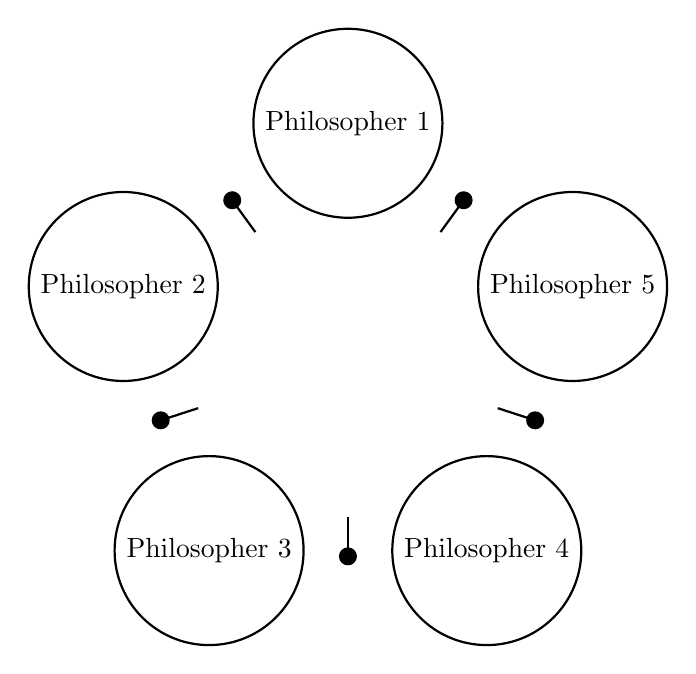
\begin{tikzpicture}

    % Draw the philosophers
    \foreach \angle/\name in {90/Philosopher 1, 162/Philosopher 2, 234/Philosopher 3, 306/Philosopher 4, 18/Philosopher 5} {
        \draw[thick] (\angle:3cm) circle (1.2cm); % Larger circle for philosophers
        \node at (\angle:3cm) {\name}; % Philosopher label
    }

    % Draw the forks between the philosophers
    \foreach \angle in {126, 198, 270, 342, 54} {
        \draw[thick] (\angle:2cm) -- (\angle:2.5cm); % Fork handle
        \draw[thick, fill=black] (\angle:2.5cm) circle (0.1cm); % Fork tip
    }

\end{tikzpicture}
\end{center}

Each philosopher is either thinking or eating, but the philosopher needs to take
\textit{both} forks to eat. The problem is to design a solution that ensures one
or more philosophers can eat when they want to. \\

A possible failing scenario is when \textit{all} philosophers take the fork to
their left. Now every philosopher is stuck waiting for the fork to their right, 
and every philosopher starve.

\section{Design}

Every philosopher behaves similarly:
\begin{itemize}
    \item Take one fork 
    \item Take another fork 
    \item Eat
    \item Put away one fork
    \item Put away another fork
\end{itemize}

\section{Spec}

The core part of \textit{Spec} looks like this: 
\\
\begin{tla}
Next ==
    \/ \E k \in 0.. P-1:
        TakeFirst(k)
    \/ \E k \in 0.. P-1:
        TakeSecond(k)
    \/ \E k \in 0.. P-1:
        Eat(k)
    \/ \E k \in 0.. P-1:
        PutFirst(k)
    \/ \E k \in 0.. P-1:
        PutSecond(k)
\end{tla}
\begin{tlatex}
\@x{ Next \.{\defeq}}%
\@x{\@s{16.4} \.{\lor} \E\, k \.{\in} 0 \.{\dotdot} P \.{-} 1 \.{:}}%
\@x{\@s{20.5} TakeFirst ( k )}%
\@x{\@s{16.4} \.{\lor} \E\, k \.{\in} 0 \.{\dotdot} P \.{-} 1 \.{:}}%
\@x{\@s{20.5} TakeSecond ( k )}%
\@x{\@s{16.4} \.{\lor} \E\, k \.{\in} 0 \.{\dotdot} P \.{-} 1 \.{:}}%
\@x{\@s{20.5} Eat ( k )}%
\@x{\@s{16.4} \.{\lor} \E\, k \.{\in} 0 \.{\dotdot} P \.{-} 1 \.{:}}%
\@x{\@s{20.5} PutFirst ( k )}%
\@x{\@s{16.4} \.{\lor} \E\, k \.{\in} 0 \.{\dotdot} P \.{-} 1 \.{:}}%
\@x{\@s{20.5} PutSecond ( k )}%
\end{tlatex}
\\

This reflects the behavior described earlier. Note that there's a sequential
dependency to these actions. The philosopher can only take the second fork after
taking the first fork, eat after having both forks and put away the forks after
eating.\\

\begin{tla}

First(k) == k
Second(k) == (k+1)% P

TakeFirst(k) == 
    /\ eaten[k] = 0
    /\ forks[First(k)] = UNUSED
    /\ UNCHANGED eaten

TakeSecond(k) ==
    /\ eaten[k] = 0
    /\ forks[First(k)] = k
    /\ forks[Second(k)] = UNUSED
    /\ forks' = [forks EXCEPT ![Second(k)] = k]
    /\ UNCHANGED eaten
\end{tla}
\begin{tlatex}
\@x{ First ( k ) \.{\defeq} k}%
\@x{ Second ( k ) \.{\defeq} ( k \.{+} 1 ) \.{\%} P}%
\@pvspace{8.0pt}%
\@x{ TakeFirst ( k ) \.{\defeq}}%
\@x{\@s{16.4} \.{\land} eaten [ k ] \.{=} 0}%
\@x{\@s{16.4} \.{\land} forks [ First ( k ) ] \.{=} UNUSED}%
\@x{\@s{16.4} \.{\land} {\UNCHANGED} eaten}%
\@pvspace{8.0pt}%
\@x{ TakeSecond ( k ) \.{\defeq}}%
\@x{\@s{16.4} \.{\land} eaten [ k ] \.{=} 0}%
\@x{\@s{16.4} \.{\land} forks [ First ( k ) ] \.{=} k}%
\@x{\@s{16.4} \.{\land} forks [ Second ( k ) ] \.{=} UNUSED}%
 \@x{\@s{16.4} \.{\land} forks \.{'} \.{=} [ forks {\EXCEPT} {\bang} [ Second
 ( k ) ] \.{=} k ]}%
\@x{\@s{16.4} \.{\land} {\UNCHANGED} eaten}%
\end{tlatex}
\\

The philosopher greedily takes the first fork when possible. After the
philosopher has the first fork, she greedily takes the second fork when
possible.
\\

\begin{tla}
Eat(k) == 
    LET 
        left == k 
        right == (k+1) % P
    IN 
        /\ forks[left] = k
        /\ forks[right] = k
        /\ eaten' = [eaten EXCEPT ![k] = 1]
        /\ UNCHANGED forks 
\end{tla}
\begin{tlatex}
\@x{ Eat ( k ) \.{\defeq}}%
\@x{ \.{\LET}}%
\@x{\@s{16.4} left \.{\defeq} k}%
\@x{\@s{16.4} right \.{\defeq} ( k \.{+} 1 ) \.{\%} P}%
\@x{ \.{\IN}}%
\@x{\@s{16.4} \.{\land} forks [ left ] \.{=} k}%
\@x{\@s{16.4} \.{\land} forks [ right ] \.{=} k}%
 \@x{\@s{16.4} \.{\land} eaten \.{'} \.{=} [ eaten {\EXCEPT} {\bang} [ k ]
 \.{=} 1 ]}%
\@x{\@s{16.4} \.{\land} {\UNCHANGED} forks}%
\end{tlatex}
\\

Once the philosopher has both forks, she can eat. 
\\
\begin{tla}
PutFirst(k) == 
    /\ eaten[k] = 1
    /\ forks[First(k)] = k 
    /\ forks' = [forks EXCEPT ![First(k)] = UNUSED]
    /\ UNCHANGED eaten

PutSecond(k) == 
    /\ eaten[k] = 1
    /\ forks[First(k)] # k 
    /\ forks[Second(k)] = k 
    /\ forks' = [forks EXCEPT ![Second(k)] = UNUSED]
    /\ eaten' = [eaten EXCEPT ![k] = 0]
\end{tla}
\begin{tlatex}
\@x{ PutFirst ( k ) \.{\defeq}}%
\@x{\@s{16.4} \.{\land} eaten [ k ] \.{=} 1}%
\@x{\@s{16.4} \.{\land} forks [ First ( k ) ] \.{=} k}%
 \@x{\@s{16.4} \.{\land} forks \.{'} \.{=} [ forks {\EXCEPT} {\bang} [ First (
 k ) ] \.{=} UNUSED ]}%
\@x{\@s{16.4} \.{\land} {\UNCHANGED} eaten}%
\@pvspace{8.0pt}%
\@x{ PutSecond ( k ) \.{\defeq}}%
\@x{\@s{16.4} \.{\land} eaten [ k ] \.{=} 1}%
\@x{\@s{16.4} \.{\land} forks [ First ( k ) ] \.{\neq} k}%
\@x{\@s{16.4} \.{\land} forks [ Second ( k ) ] \.{=} k}%
 \@x{\@s{16.4} \.{\land} forks \.{'} \.{=} [ forks {\EXCEPT} {\bang} [ Second
 ( k ) ] \.{=} UNUSED ]}%
 \@x{\@s{16.4} \.{\land} eaten \.{'} \.{=} [ eaten {\EXCEPT} {\bang} [ k ]
 \.{=} 0 ]}%
\end{tlatex}
\\

After eating, the philosopher puts away the forks.

\section{Safety}

Omitted for this chapter.

\section{Liveness}

One liveness property is to ensure that at least one philosopher can eat when she
wants to under all circumstances:\\

\begin{tla}
Liveness ==
    \E k \in 0..P-1:
        /\ eaten[k] = 0 ~> eaten[k] = 1
        /\ eaten[k] = 1 ~> eaten[k] = 0
\end{tla}
\begin{tlatex}
\@x{ Liveness \.{\defeq}}%
\@x{\@s{16.4} \E\, k \.{\in} 0 \.{\dotdot} P \.{-} 1 \.{:}}%
\@x{\@s{20.5} \.{\land} eaten [ k ] \.{=} 0 \.{\leadsto} eaten [ k ] \.{=} 1}%
\@x{\@s{20.5} \.{\land} eaten [ k ] \.{=} 1 \.{\leadsto} eaten [ k ] \.{=} 0}%
\end{tlatex}
\\

However, \textit{Spec} defined as is doesn't implement any deadlock mitigation.
Running it against the model the checker results in the following violations: 

\begin{verbatim}
State 2: <TakeFirst line 19, col 5 to line 23, 
    col 22 of module dining>
/\ eaten = (0 :> 0 @@ 1 :> 0 @@ 2 :> 0)
/\ forks = (0 :> 0 @@ 1 :> 100 @@ 2 :> 100)

State 3: <TakeFirst line 19, col 5 to line 23, 
    col 22 of module dining>
/\ eaten = (0 :> 0 @@ 1 :> 0 @@ 2 :> 0)
/\ forks = (0 :> 0 @@ 1 :> 1 @@ 2 :> 100)

State 4: <TakeFirst line 19, col 5 to line 23, 
    col 22 of module dining>
/\ eaten = (0 :> 0 @@ 1 :> 0 @@ 2 :> 0)
/\ forks = (0 :> 0 @@ 1 :> 1 @@ 2 :> 2)
\end{verbatim}

When all philosopher takes their left fork, no one can eat. \\

A simple fix to the problem is for every philosopher to take the fork with the
smaller index first:\\

\begin{tla}
First(k) == IF k # P-1 THEN k ELSE 0
Second(k) == IF k # P-1 THEN k+1 ELSE k
\end{tla}
\begin{tlatex}
 \@x{ First ( k ) \.{\defeq} {\IF} k \.{\neq} P \.{-} 1 \.{\THEN} k \.{\ELSE}
 0}%
 \@x{ Second ( k ) \.{\defeq} {\IF} k \.{\neq} P \.{-} 1 \.{\THEN} k \.{+} 1
 \.{\ELSE} k}%
\end{tlatex}
\\

When the philosopher with the highest index wants to eat, she will need to take
fork 0 first. In the case where all other philosophers have already taken their
first fork, the philosopher with the highest index will fail to take her first
fork (because it has already been taken by the first philosopher). This allows
the philosopher with the second-highest index to make progress, thus preventing a
deadlock.\\

The model checker will pass the updated \textit{Spec}.

% \end{document}


% \begin{document}

\chapter{Strongly Connected Components}

In a graph, a strongly connected component (SCC) is a subset of vertices where
every pair of vertices are reachable from each other. An example graph with four
SCCs is illustrated below, where the vertices that share the same color and belong in the
same SCC:\\

\begin{center}
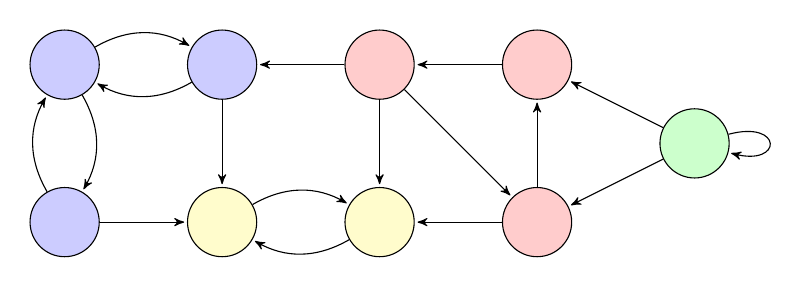
\begin{tikzpicture}[->, >=stealth', shorten >=1pt, auto, node distance=2cm]

  % Define nodes

  \node[state, fill=blue!20] (n1) at (0, 0)  {};
  \node[state, fill=blue!20] (n2) at (0, -2) {};
  \node[state, fill=blue!20] (n3) at (2, 0)  {};

  \node[state, fill=yellow!20] (n4) at (2, -2) {};

  \node[state, fill=red!20] (n5) at (4, 0)  {};
  \node[state, fill=yellow!20] (n6) at (4, -2) {};

  \node[state, fill=red!20] (n7) at (6, 0)  {};
  \node[state, fill=red!20] (n8) at (6, -2) {};

  \node[state, fill=green!20] (n9) at (8, -1) {};

  % Draw edges
  \draw[->] (n1) edge[bend left] (n2);
  \draw[->] (n2) edge[bend left] (n1);

  \draw[->] (n1) edge[bend left] (n3);
  \draw[->] (n3) edge[bend left] (n1);

  \draw[->] (n3) edge[] (n4);
  \draw[->] (n2) edge[] (n4);

  \draw[->] (n4) edge[bend left] (n6);
  \draw[->] (n6) edge[bend left] (n4);

  \draw[->] (n5) edge[] (n3);
  \draw[->] (n5) edge[] (n6);
  \draw[->] (n5) edge[] (n8);

  \draw[->] (n7) edge[] (n5);

  \draw[->] (n8) edge[] (n6);
  \draw[->] (n8) edge[] (n7);

  \draw[->] (n9) edge[] (n7);
  \draw[->] (n9) edge[] (n8);
  
  \draw[->] (n9) edge[loop right] (n9);

\end{tikzpicture}
\end{center}

A node is an SCC by itself. There are many applications of SCCs, including:
social network analysis, web crawling, and software modularity analysis.\\

TLA+ also uses SCCs to verify the liveness properties of a specification.
Consider the following graph from a hypothetical specification: 

\begin{center}
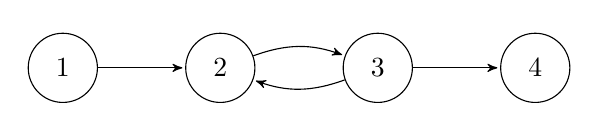
\begin{tikzpicture}[>=stealth',shorten >=1pt,auto,node distance=2cm]
  \node[state]  (q1)                {1};
  \node[state]  (q2) [right of=q1]  {2};
  \node[state]  (q3) [right of=q2]  {3};
  \node[state]  (q4) [right of=q3]  {4};

  \path[->]          (q1) edge   []   node {} (q2);

  \path[->]          (q2) edge   [bend left=20]   node {} (q3);
  \path[->]          (q3) edge   [bend left=20]   node {} (q2);
  
  \path[->]          (q3) edge   []   node {} (q4);
\end{tikzpicture}
\end{center}

States 2 and 3 form an SCC. Assume the system has a liveness property that
defines state 1 \textit{leads to} state 4. The model checker can fail the specification
because execution may be trapped inside the SSC (unless a fairness description
is provided). The model checker must first identify all SCCs in the graph to
verify liveness. This explains why verifying liveness non-trivially increases
model checker runtime, because the SCC identifying algorithm implemented in the
model checker runs linearly.\\

In this chapter, we will implement a horizontally scalable SCC detection
algorithm described in \textit{A GPU Algorithm for Detecting Strongly Connected
Components} \cite{gpu_scc}.

\section{Design}

The following provides the pseudocode description of the parallel SCC detection
algorithm as described in the paper:\\

\makeatletter
\algnewcommand{\LineComment}[1]{\Statex \hskip\ALG@thistlm \(\triangleright\) #1}
\makeatother

\begin{algorithmic}[1]

\State $converged \gets false$

\While{not $converged$}
    
    \LineComment{Initialize vertex}
    \ForAll{vertices $v \in V$}
        \State $v_{in} \gets v_{id}$
        \State $v_{out} \gets v_{id}$
    \EndFor

    \LineComment{Propagate max value}
    \State $updated \gets false$
    \While{$updated$}
        \ForAll{edges $(u -> v)\in E$}
            \State $v_{out} \gets max(u_{out},v_{out})$
            \State $v_{in} \gets max(u_{in},v_{in})$
        \EndFor
        \State $updated \gets$ at least one $v_{in}$ or $v_{out}$ value changed 
    \EndWhile

    \LineComment{Remove edges that span SCC}
    \ForAll{edges $(u \rightarrow v)\in E$}
        \If {$u_{in} \neq v_{in}$ or $u_{out} \neq v_{out}$}
            \State $E \gets E \ (u \rightarrow v)$
        \EndIf
    \EndFor

\EndWhile
\end{algorithmic}

The algorithm is split into three parts: initialization, max value
propagation and edge trimming.

\section{Specification}

\textit{Spec} is defined into three phases: \textit{Init}, \textit{Update},
\textit{Trim}. Phase \textit{Init} is defined as follow:\\
\begin{tla}
PhaseInit == 
    /\ phase = "Init" 
    /\ phase' = "Update"
    /\ edges' = new_edges
    /\ new_edges' = new_edges
    /\ in' = [k \in Vertex |-> k]
    /\ out' = [k \in Vertex |-> k]
    /\ updated' = 0
    /\ converged' = 0
\end{tla}
\begin{tlatex}
\@x{ PhaseInit \.{\defeq}}%
\@x{\@s{16.4} \.{\land} phase \.{=}\@w{Init}}%
\@x{\@s{16.4} \.{\land} phase \.{'} \.{=}\@w{Update}}%
\@x{\@s{16.4} \.{\land} edges \.{'} \.{=} new\_edges}%
\@x{\@s{16.4} \.{\land} new\_edges \.{'} \.{=} new\_edges}%
\@x{\@s{16.4} \.{\land} in \.{'} \.{=} [ k \.{\in} Vertex \.{\mapsto} k ]}%
\@x{\@s{16.4} \.{\land} out \.{'} \.{=} [ k \.{\in} Vertex \.{\mapsto} k ]}%
\@x{\@s{16.4} \.{\land} updated \.{'} \.{=} 0}%
\@x{\@s{16.4} \.{\land} converged \.{'} \.{=} 0}%
\end{tlatex}\\

\textit{in} and \textit{out} are defined as lookup table using
\textit{functions}.\\

\pagebreak

The \textit{Update} phase implements max value propagation:\\
\begin{tla}
PhaseUpdate == 
    /\ phase = "Update"
    /\ \/ /\ \E e \in edges: 
            LET 
                src == e[1]
                dst == e[2]
            IN 
                /\ in' = [in EXCEPT ![dst] = Max(in[src], in[dst])]
                /\ out' = [out EXCEPT ![src] = Max(out[src], out[dst])]
                /\ edges' = edges \ {e}
                /\ \/ /\ in' # in \/ out' # out
                      /\ updated' = 1
                   \/ /\ in' = in /\ out' = out
                      /\ updated' = 0
          /\ UNCHANGED <<new_edges, phase, converged>>
       \/ /\ edges = {}
          /\ updated = 0
          /\ phase' = "Trim"
          /\ UNCHANGED <<edges, new_edges, in, out, updated, converged>>
       \/ /\ edges = {}
          /\ updated # 0
          /\ edges' = new_edges
          /\ UNCHANGED <<phase, new_edges, in, out, updated, converged>>
\end{tla}
\begin{tlatex}
\@x{ PhaseUpdate \.{\defeq}}%
\@x{\@s{16.4} \.{\land} phase \.{=}\@w{Update}}%
\@x{\@s{16.4} \.{\land} \.{\lor} \.{\land} \E\, e \.{\in} edges \.{:}}%
\@x{\@s{24.59} \.{\LET}}%
\@x{\@s{41.0} src \.{\defeq} e [ 1 ]}%
\@x{\@s{41.0} dst \.{\defeq} e [ 2 ]}%
\@x{\@s{24.59} \.{\IN}}%
 \@x{\@s{41.0} \.{\land} in \.{'} \.{=} [ in {\EXCEPT} {\bang} [ dst ] \.{=}
 Max ( in [ src ] ,\, in [ dst ] ) ]}%
 \@x{\@s{41.0} \.{\land} out \.{'} \.{=} [ out {\EXCEPT} {\bang} [ src ] \.{=}
 Max ( out [ src ] ,\, out [ dst ] ) ]}%
\@x{\@s{41.0} \.{\land} edges \.{'} \.{=} edges \.{\,\backslash\,} \{ e \}}%
 \@x{\@s{41.0} \.{\land} \.{\lor} \.{\land} in \.{'} \.{\neq} in \.{\lor} out
 \.{'} \.{\neq} out}%
\@x{\@s{41.0} \.{\land} updated \.{'} \.{=} 1}%
 \@x{\@s{41.0} \.{\lor} \.{\land} in \.{'} \.{=} in \.{\land} out \.{'} \.{=}
 out}%
\@x{\@s{41.0} \.{\land} updated \.{'} \.{=} 0}%
 \@x{\@s{16.4} \.{\land} {\UNCHANGED} {\langle} new\_edges ,\, phase ,\,
 converged {\rangle}}%
\@x{\@s{16.4} \.{\lor} \.{\land} edges \.{=} \{ \}}%
\@x{\@s{16.4} \.{\land} updated \.{=} 0}%
\@x{\@s{16.4} \.{\land} phase \.{'} \.{=}\@w{Trim}}%
 \@x{\@s{16.4} \.{\land} {\UNCHANGED} {\langle} edges ,\, new\_edges ,\, in
 ,\, out ,\, updated ,\, converged {\rangle}}%
\@x{\@s{16.4} \.{\lor} \.{\land} edges \.{=} \{ \}}%
\@x{\@s{16.4} \.{\land} updated \.{\neq} 0}%
\@x{\@s{16.4} \.{\land} edges \.{'} \.{=} new\_edges}%
 \@x{\@s{16.4} \.{\land} {\UNCHANGED} {\langle} phase ,\, new\_edges ,\, in
 ,\, out ,\, updated ,\, converged {\rangle}}%
\end{tlatex}
\\

The edge iteration loop is implemented with an existential qualifier over edges.
After processing an edge, the edge is removed from the set edges to simulate so
it is not chosen again in the next iteration. Once set edges become empty, the
algorithm determines if we need to repeat the propagation process.\\

\pagebreak

The following implements phase \textit{trim}:\\
\begin{tla}
PhaseTrim == 
    /\ phase = "Trim"
    /\ \/ /\ edges = {}
          /\ in = out
          /\ converged' = 1
          /\ UNCHANGED <<phase, new_edges, edges, in, out, updated>>
       \/ /\ edges = {}
          /\ in # out
          /\ phase' = "Init"
          /\ UNCHANGED <<in, new_edges, edges, out, updated, converged>>
       \/ /\ edges # {}
          /\ \E e \in edges:
            LET 
                src == e[1]
                dst == e[2]
            IN
                /\ \/ /\ out[src] # out[dst] \/ in[src] # in[dst]
                      /\ new_edges' = new_edges \ {e}
                   \/ /\ out[src] = out[dst] /\ in[src] = in[dst]
                      /\ UNCHANGED new_edges
                /\ edges' = edges \ {e}
          /\ UNCHANGED <<phase, in, out, updated, converged>>
\end{tla}
\begin{tlatex}
\@x{ PhaseTrim \.{\defeq}}%
\@x{\@s{16.4} \.{\land} phase \.{=}\@w{Trim}}%
\@x{\@s{16.4} \.{\land} \.{\lor} \.{\land} edges \.{=} \{ \}}%
\@x{\@s{16.4} \.{\land} in \.{=} out}%
\@x{\@s{16.4} \.{\land} converged \.{'} \.{=} 1}%
 \@x{\@s{16.4} \.{\land} {\UNCHANGED} {\langle} phase ,\, new\_edges ,\, edges
 ,\, in ,\, out ,\, updated {\rangle}}%
\@x{\@s{16.4} \.{\lor} \.{\land} edges \.{=} \{ \}}%
\@x{\@s{16.4} \.{\land} in \.{\neq} out}%
\@x{\@s{16.4} \.{\land} phase \.{'} \.{=}\@w{Init}}%
 \@x{\@s{16.4} \.{\land} {\UNCHANGED} {\langle} in ,\, new\_edges ,\, edges
 ,\, out ,\, updated ,\, converged {\rangle}}%
\@x{\@s{16.4} \.{\lor} \.{\land} edges \.{\neq} \{ \}}%
\@x{\@s{16.4} \.{\land} \E\, e \.{\in} edges \.{:}}%
\@x{\@s{24.59} \.{\LET}}%
\@x{\@s{41.0} src \.{\defeq} e [ 1 ]}%
\@x{\@s{41.0} dst \.{\defeq} e [ 2 ]}%
\@x{\@s{24.59} \.{\IN}}%
 \@x{\@s{41.0} \.{\land} \.{\lor} \.{\land} out [ src ] \.{\neq} out [ dst ]
 \.{\lor} in [ src ] \.{\neq} in [ dst ]}%
 \@x{\@s{41.0} \.{\land} new\_edges \.{'} \.{=} new\_edges \.{\,\backslash\,}
 \{ e \}}%
 \@x{\@s{41.0} \.{\lor} \.{\land} out [ src ] \.{=} out [ dst ] \.{\land} in [
 src ] \.{=} in [ dst ]}%
\@x{\@s{41.0} \.{\land} {\UNCHANGED} new\_edges}%
\@x{\@s{41.0} \.{\land} edges \.{'} \.{=} edges \.{\,\backslash\,} \{ e \}}%
 \@x{\@s{16.4} \.{\land} {\UNCHANGED} {\langle} phase ,\, in ,\, out ,\,
 updated ,\, converged {\rangle}}%
\end{tlatex}
\\

Similar to the previous phase, we use existential qualifiers and set subtraction to
simulate iterating through all edges. Another variable \textit{new\_edges} is
used to track edges to be used in the next iteration if required. 

\section{Safety}

To find the solution of a given graph, let us define a safety property where
converged is always 0:\\

\begin{tla}
Termination == 
    converged = 0
\end{tla}
\begin{tlatex}
\@x{ Termination \.{\defeq}}%
\@x{\@s{16.4} converged \.{=} 0}%
\end{tlatex}

In other words, we want the model checker to terminate when converged becomes 1.\\ 

Let us assume input similar to as defined in the paper:

\begin{center}
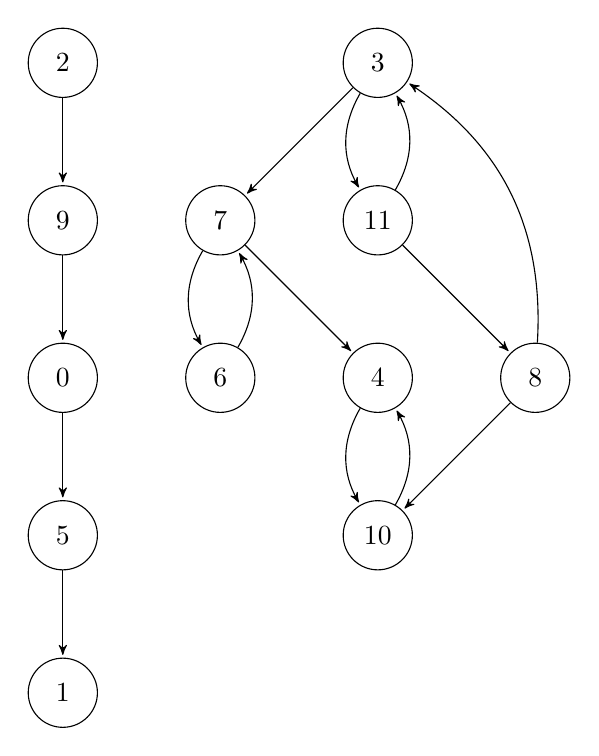
\begin{tikzpicture}[->, >=stealth', shorten >=1pt, auto, node distance=2cm]

  % Define nodes

  \node[state] (n2) at (0, 0)  {2};
  \node[state] (n9) at (0, -2) {9};
  \node[state] (n0) at (0, -4) {0};
  \node[state] (n5) at (0, -6) {5};
  \node[state] (n1) at (0, -8) {1};

  \node[state] (n3) at (4, 0) {3};
  \node[state] (n11) at (4, -2) {11};
  \node[state] (n7) at (2, -2) {7};
  \node[state] (n4) at (4, -4) {4};
  \node[state] (n6) at (2, -4) {6};
  \node[state] (n10) at (4, -6) {10};
  \node[state] (n8) at (6, -4) {8};

  % Draw edges
  \draw[->] (n2) edge[] (n9);
  \draw[->] (n9) edge[] (n0);
  \draw[->] (n0) edge[] (n5);
  \draw[->] (n5) edge[] (n1);

  \draw[->] (n3) edge[] (n7);
  \draw[->] (n3) edge[bend right] (n11);

  \draw[->] (n6) edge[bend right] (n7);

  \draw[->] (n7) edge[bend right] (n6);
  \draw[->] (n7) edge[] (n4);

  \draw[->] (n8) edge[] (n10);
  \draw[->] (n8) edge[bend right] (n3);

  \draw[->] (n4) edge[bend right] (n10);

  \draw[->] (n10) edge[bend right] (n4);

  \draw[->] (n11) edge[] (n8);
  \draw[->] (n11) edge[bend right] (n3);

%   \draw[->] (n2) edge[bend left] (n1);

%   \draw[->] (n1) edge[bend left] (n3);
%   \draw[->] (n3) edge[bend left] (n1);

%   \draw[->] (n3) edge[] (n4);
%   \draw[->] (n2) edge[] (n4);

%   \draw[->] (n4) edge[bend left] (n6);
%   \draw[->] (n6) edge[bend left] (n4);

%   \draw[->] (n5) edge[] (n3);
%   \draw[->] (n5) edge[] (n6);
%   \draw[->] (n5) edge[] (n8);

%   \draw[->] (n7) edge[] (n5);

%   \draw[->] (n8) edge[] (n6);
%   \draw[->] (n8) edge[] (n7);

%   \draw[->] (n9) edge[] (n7);
%   \draw[->] (n9) edge[] (n8);
  
%   \draw[->] (n9) edge[loop right] (n9);

\end{tikzpicture}
\end{center}

Running the model checker against the specification outputs the following: 
\begin{verbatim}
Error: Invariant Termination is violated.                               
Error: The behavior up to this point is:      
...
State 15: <PhaseTrim line 76, col 5 to line 96, 
    col 61 of module scc>
/\ out = ( 0 :> 0 @@ 
  1 :> 1 @@  
  2 :> 2 @@ 
  3 :> 11 @@                                                            
  4 :> 10 @@                                                            
  5 :> 5 @@                                                             
  6 :> 7 @@                                                             
  7 :> 7 @@                                                             
  8 :> 11 @@                                                            
  9 :> 9 @@                                                             
  10 :> 10 @@                                                           
  11 :> 11 )   
...
\end{verbatim}

As defined by the algorithm, vertices sharing the same value are part of the
same SCC. The specification correctly identifies three SCCs with more than one vertex:
\{3, 8, 11\}, \{6, 7\} and \{4, 10\}.

\section{Liveness}

Omitted for this chapter.

% \end{document}


\chapter{Simple Scheduler}

\section{Requirement}

In this section we will define a spec for a simple task scheduler. The task sechdeuler has the following
requirements:
\begin{itemize}
    \item Supporting N execution context (ie. CPUs)
    \item Supporting T number of tasks
    \item Tasks have identical priority and are scheduled coopertively
    \item System has a single global lock
    \item Any task can attempt to acquire the lock, Any task attempting to
    acquire the lock are gauranteed to be scheduled.
    \item If multiple tasks attempt to grab the lock, the tasks will be
    scheduled in lock request order. 
\end{itemize}

\section{Spec}

We will model scheduler using the following variables:\newline
\begin{tla}
Init ==
    /\ cpus = [i \in 0..N-1 |-> ""] 
    /\ ready_q = S2T(Tasks)
    /\ blocked_q = <<>>
    /\ lock_owner = ""
\end{tla}
\begin{tlatex}
\@x{ Init \.{\defeq}}%
 \@x{\@s{16.4} \.{\land} cpus \.{=} [ i \.{\in} 0 \.{\dotdot} N \.{-} 1
 \.{\mapsto}\@w{} ]}%
\@x{\@s{16.4} \.{\land} ready\_q \.{=} S2T ( Tasks )}%
\@x{\@s{16.4} \.{\land} blocked\_q \.{=} {\langle} {\rangle}}%
\@x{\@s{16.4} \.{\land} lock\_owner \.{=}\@w{}}%
\end{tlatex}
\newline

A few things to note:
\begin{itemize}
    \item The system has $N$ executing context, represented as number of CPUs.
    When a task is running, $cpus[k]$ is set to $taskName$. When CPU is idle,
    $cpus[k]$ is set to an empty string. 
    \item $ready\_q$ and $blocked\_q$ are initialized as \textit{ordered tuple},
    due to the cooperative scheduling requirement.
    \item $S2T$ is a macro that converts a set into a ordered tuple. This is to
    accommodate the fact it appears I cannot define tuple in .cfg file.
    \item Finally, the single system lock is represented as $lock\_owner$. 
\end{itemize}

A task can be in three possible state: Ready, Blocked and Running. The $Next$
box-action fomula will define a Ready and Running action, and the implementation
will include related lock contention handling.\newline

\begin{tla}
------- MODULE scheduler ---- 
MoveToReady(k) == 
    /\ cpus[k] # "" 
    /\ lock_owner # cpus[k]
    /\ ready_q' = Append(ready_q, cpus[k]) 
    /\ cpus' = [cpus EXCEPT ![k] = ""]
    /\ UNCHANGED <<lock_owner, blocked_q>>
Lock(k) == 
    \* lock is empty
    \/  /\ cpus[k] # "" 
        /\ lock_owner = ""
        /\ lock_owner' = cpus[k]
        /\ UNCHANGED <<ready_q, cpus, blocked_q>>
    \* someone else has the lock
    \/  /\ cpus[k] # "" 
        /\ lock_owner # ""
        /\ lock_owner # cpus[k] \* cannot double lock
        /\ blocked_q' = Append(blocked_q, cpus[k])
        /\ cpus' = [cpus EXCEPT ![k] = ""]
        /\ UNCHANGED <<ready_q, lock_owner>>
Unlock(k) == 
    /\ cpus[k] # "" 
    /\ lock_owner = cpus[k]
    /\ lock_owner' = ""
    /\ cpus' = [cpus EXCEPT ![k] = ""]
    /\ ready_q' = ready_q \o blocked_q \o <<cpus[k]>>
    /\ blocked_q' = <<>>

Running == 
    \E k \in DOMAIN cpus:
        /\ cpus[k] # "" 
        /\ \/ MoveToReady(k)
           \/ Lock(k)
           \/ Unlock(k)
=============================================================================
\end{tla}
\begin{tlatex}
\@x{}\moduleLeftDash\@xx{ {\MODULE} scheduler}\moduleRightDash\@xx{}%
\@x{ MoveToReady ( k ) \.{\defeq}}%
\@x{\@s{16.4} \.{\land} cpus [ k ] \.{\neq}\@w{}}%
\@x{\@s{16.4} \.{\land} lock\_owner \.{\neq} cpus [ k ]}%
 \@x{\@s{16.4} \.{\land} ready\_q \.{'} \.{=} Append ( ready\_q ,\, cpus [ k ]
 )}%
 \@x{\@s{16.4} \.{\land} cpus \.{'} \.{=} [ cpus {\EXCEPT} {\bang} [ k ]
 \.{=}\@w{} ]}%
 \@x{\@s{16.4} \.{\land} {\UNCHANGED} {\langle} lock\_owner ,\, blocked\_q
 {\rangle}}%
\@x{ Lock ( k ) \.{\defeq}}%
\@x{\@s{20.63}}%
\@y{%
  lock is empty
}%
\@xx{}%
\@x{\@s{20.63} \.{\lor}\@s{4.1} \.{\land} cpus [ k ] \.{\neq}\@w{}}%
\@x{\@s{35.84} \.{\land} lock\_owner \.{=}\@w{}}%
\@x{\@s{35.84} \.{\land} lock\_owner \.{'} \.{=} cpus [ k ]}%
 \@x{\@s{35.84} \.{\land} {\UNCHANGED} {\langle} ready\_q ,\, cpus ,\,
 blocked\_q {\rangle}}%
\@x{\@s{20.63}}%
\@y{%
  someone else has the lock
}%
\@xx{}%
\@x{\@s{20.63} \.{\lor}\@s{4.1} \.{\land} cpus [ k ] \.{\neq}\@w{}}%
\@x{\@s{35.84} \.{\land} lock\_owner \.{\neq}\@w{}}%
\@x{\@s{35.84} \.{\land} lock\_owner \.{\neq} cpus [ k ]}%
\@y{%
  cannot double lock
}%
\@xx{}%
 \@x{\@s{35.84} \.{\land} blocked\_q \.{'}\@s{5.22} \.{=} Append ( blocked\_q
 ,\, cpus [ k ] )}%
 \@x{\@s{35.84} \.{\land} cpus \.{'} \.{=} [ cpus {\EXCEPT} {\bang} [ k ]
 \.{=}\@w{} ]}%
 \@x{\@s{35.84} \.{\land} {\UNCHANGED} {\langle} ready\_q ,\, lock\_owner
 {\rangle}}%
\@x{ Unlock ( k ) \.{\defeq}}%
\@x{\@s{16.4} \.{\land} cpus [ k ] \.{\neq}\@w{}}%
\@x{\@s{16.4} \.{\land} lock\_owner \.{=} cpus [ k ]}%
\@x{\@s{16.4} \.{\land} lock\_owner \.{'} \.{=}\@w{}}%
 \@x{\@s{16.4} \.{\land} cpus \.{'} \.{=} [ cpus {\EXCEPT} {\bang} [ k ]
 \.{=}\@w{} ]}%
 \@x{\@s{16.4} \.{\land} ready\_q \.{'} \.{=} ready\_q \.{\circ} blocked\_q
 \.{\circ} {\langle} cpus [ k ] {\rangle}}%
\@x{\@s{16.4} \.{\land} blocked\_q \.{'} \.{=} {\langle} {\rangle}}%
\@pvspace{8.0pt}%
\@x{ Running \.{\defeq}}%
\@x{\@s{16.4} \E\, k \.{\in} {\DOMAIN} cpus \.{:}}%
\@x{\@s{27.72} \.{\land} cpus [ k ] \.{\neq}\@w{}}%
\@x{\@s{27.72} \.{\land} \.{\lor} MoveToReady ( k )}%
\@x{\@s{38.83} \.{\lor} Lock ( k )}%
\@x{\@s{38.83} \.{\lor} Unlock ( k )}%
\@x{}\bottombar\@xx{}%
\end{tlatex}

\section{Safety}

\section{Liveness}

I believe this is the most important part of cooperative scheduler design. While
the scheduler can't \textit{force} a task to relinquish a lock (the scheduler
doesn't dictate when the task is \textit{done}), the scheduler can ensure
scheduling fairness by scheduling the next lock requester intsead of the task 
that just relinquished the lock.\newline

\begin{tla}
----- MODULE scheduler ---- 
Liveness == 
    \A t \in Tasks:
        LET 
            b == {x \in DOMAIN blocked_q : blocked_q[x] = t}
        IN 
            /\ b # {} ~> b = {}
==========
\end{tla}
\begin{tlatex}
\@x{}\moduleLeftDash\@xx{ {\MODULE} scheduler}\moduleRightDash\@xx{}%
\@x{ Liveness \.{\defeq}}%
\@x{\@s{16.4} \A\, t \.{\in} Tasks \.{:}}%
\@x{\@s{27.72} \.{\LET}}%
 \@x{\@s{44.12} b \.{\defeq} \{ x \.{\in} {\DOMAIN} blocked\_q \.{:}
 blocked\_q [ x ] \.{=} t \}}%
\@x{\@s{27.72} \.{\IN}}%
\@x{\@s{44.12} \.{\land} b \.{\neq} \{ \} \.{\leadsto} b \.{=} \{ \}}%
\@x{}\bottombar\@xx{}%
\end{tlatex}
\newline

The formula defines set b to be either an empty set or a set of one task. Assume
a set of \{"p0", "p1", "p2\}. Possible value of b include: \{\}, \{"p0"\},
\{"p1"\} and \{"p2"\}. The fomula then states an non empty set of b leads to an
\textit{empty set} of b. In other words: \newline

\textit{If a task ever becomes blocked, it will eventually become unblocked}.\newline

However, when we actually run the model checker, we will find the liveness
property is \textit{violated}. The failure scenario is basically one task
holding onto the lock in one CPU, while the scheduler repeatedly
schedule/deschedule a separate task in another CPU. While this is perfectly
allowed, the model checker detects a possible path for the the system to trap in
a local state and fail the liveness property.\newline 

Perhaps not surprisingly, if you construct similar liveness property to verify 
a task is \textit{eventually} always scheduled, it will also fail. The model
checker will provide a counter case where a task is never scheduled because
another task is repeatedly acquire/release the global lock.\newline

We need \textit{Strong Fairness} to solve this problem:
\begin{tla}
----- MODULE scheduler ---- 
L ==
    \A t \in Tasks :
        \A n \in 0..(N-1) :
            WF_vars(HoldingLock(t) /\ Unlock(n))
Spec ==
  /\ Init
  /\ [][Next]_vars
  /\ WF_vars(Next)
  /\ L 
======= 
\end{tla}
\begin{tlatex}
\@x{}\moduleLeftDash\@xx{ {\MODULE} scheduler}\moduleRightDash\@xx{}%
\@x{ L \.{\defeq}}%
\@x{\@s{14.47} \A\, t \.{\in} Tasks \.{:}}%
\@x{\@s{25.79} \A\, n \.{\in} 0 \.{\dotdot} ( N \.{-} 1 ) \.{:}}%
\@x{\@s{37.11} {\WF}_{ vars} ( HoldingLock ( t ) \.{\land} Unlock ( n ) )}%
\@x{ Spec \.{\defeq}}%
\@x{\@s{8.2} \.{\land}\@s{0.16} Init}%
\@x{\@s{8.2} \.{\land}\@s{0.16} {\Box} [ Next ]_{ vars}}%
\@x{\@s{8.2} \.{\land}\@s{0.16} {\WF}_{ vars} ( Next )}%
\@x{\@s{8.2} \.{\land}\@s{0.16} L}%
\@x{}\bottombar\@xx{}%
\end{tlatex}
\newline

Fairness ensures that we are never stuck in a repeated state.



SPECIFICATION Spec

CONSTANTS
    Servers = {s0, s1, s2}
    \* Servers = {s0, s1}

\* INVARIANTS 
\*     TypeOK
PROPERTIES 
    Liveness


\chapter{Selective Retransmit}

Assume client device that playsback a video stream. Structurelly, a video is
composed of frames, frames are then segmented into packets to stream across a 
network. The client device recombines the packets into a frame, then sequence
the frame to playback the video.\newline

However, network is not-deterministic. Depending on the route the packets take
to get to the client, they may arrive out-of-order. The client may need to
maintain a receive buffer for the packets, re-order the packets back into
sequence before pushing the packets down to decoding engine.\newline

The network may also drop packets if any of the switches gets too busy. In the
case of a packet drop, the client has a few options. The client can either
discard the frame and let the decoding engine downstream to deal with it (which
may ressult in  visible artifacts during play back). The client can request the
whole frame to be re-sent, which results in additional bandwidith consumption.
The client can selectively request the missing packet to be retransmited, which
will minimize additional bandwidth consumption, but increases implementation 
complexity.\newline 

In this chapter, we will implement a simple selective retransmit
algorithm.\newline

\begin{center}

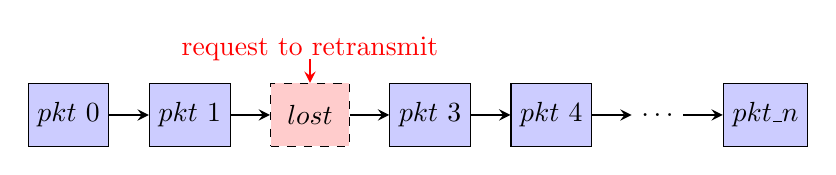
\begin{tikzpicture}[
    packet/.style={rectangle, draw, fill=blue!20, minimum width=1cm, minimum height=0.8cm},
    missing/.style={rectangle, draw, dashed, fill=red!20, minimum width=1cm, minimum height=0.8cm},
    arrow/.style={->, >=stealth, thick}
]

    % Draw packets
    \node[packet] (p0) at (0,0) {\(pkt\ 0\)};
    \node[packet, right=0.5cm of p0] (p2) {\(pkt\ 1\)};
    \node[missing, right=0.5cm of p2] (missing1) {\(lost\)};
    \node[packet, right=0.5cm of missing1] (p4) {\(pkt\ 3\)};
    \node[packet, right=0.5cm of p4] (p5) {\(pkt\ 4\)};
    \node[right=0.5cm of p5] (dots) {\(\dots\)}; % Just dots, no box
    \node[packet, right=0.5cm of dots] (pn) {\(pkt\_n\)};

    % Draw arrows between packets
    \draw[arrow] (p0.east) -- (p2.west);
    \draw[arrow] (p2.east) -- (missing1.west);
    \draw[arrow] (missing1.east) -- (p4.west);
    \draw[arrow] (p4.east) -- (p5.west);
    \draw[arrow] (p5.east) -- (dots);
    \draw[arrow] (dots) -- (pn.west);

    % Add arrow pointing to "lost" with caption
    \draw[arrow, red] ([yshift=0.3cm] missing1.north) -- (missing1.north) 
        node[midway, above, text=red] {request to retransmit};

\end{tikzpicture}

\end{center}

\section{Requirement}

Since packets may arrive out-of-order, the server stamps the packets with
sequence number to allow the client to order the packets as they arrive.
Once the client has a set of ordered packets, it moves the packets from the 
receive buffer into the decoding engine to be displayed.\newline

The video packets are often sent to client via unreliable channel to minimize
network overhead and latency. The client sends acknowledgement back to the
server via to acknowledge the received packet. This indicates to the server it
can send more video data to the client. The acknowlegements are not latency
sensitive in nature, and take up a very small proportion of bandwidth, so they
are transported through reliable channel.\newline

The following illustrates a re-ordering scenario:
\begin{center}
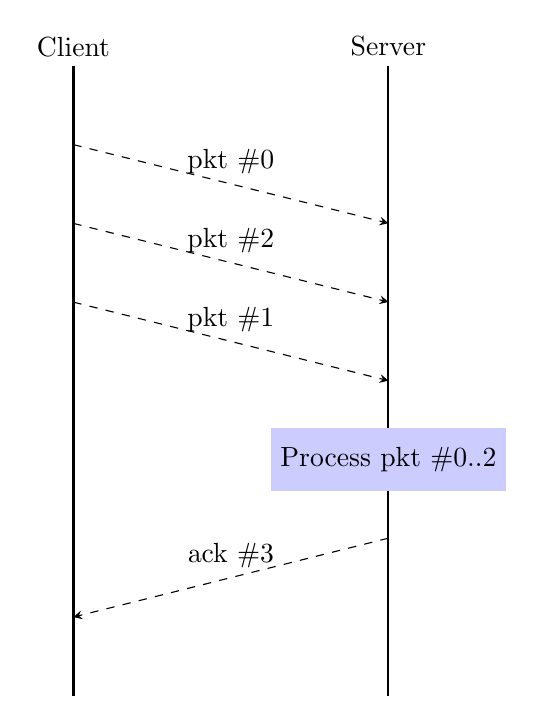
\begin{tikzpicture}[
    lifeline/.style={thick},
    message/.style={->, >=stealth, dashed},
    activation/.style={rectangle, fill=blue!20, minimum width=0.5cm, minimum height=0.8cm} ]

    % Define lifelines
    \node[] (client) at (0,0) {Client};
    \node[] (server) at (4,0) {Server};
    % \node[] (database) at (8,0) {Database};

    % Draw lifelines
    \draw[lifeline] (client.south) -- ++(0,-8);
    \draw[lifeline] (server.south) -- ++(0,-8);
    % \draw[lifeline] (database.south) -- ++(0,-8);

    % Draw messages
    \draw[message] ([yshift=-1cm] client.south) -- node[above] {pkt \#0} ([yshift=-2cm] server.south);
    \draw[message] ([yshift=-2cm] client.south) -- node[above] {pkt \#2} ([yshift=-3cm] server.south);
    \draw[message] ([yshift=-3cm] client.south) -- node[above] {pkt \#1} ([yshift=-4cm] server.south);
    % \draw[message] ([yshift=-2cm] server.south) -- node[above] {query} ([yshift=-2cm] database.south);
    % \draw[message] ([yshift=-3cm] database.south) -- node[above] {response} ([yshift=-3cm] server.south);
    \draw[message] ([yshift=-6cm] server.south) -- node[above] {ack \#3} ([yshift=-7cm] client.south);

    % \draw[message] ([yshift=-5cm] server.south) to[out=-90, in=-90, looseness=1.5] node[above] {ack \#3} ([yshift=-6cm] server.south);
    % \draw[message] ([yshift=-1cm] server.south) to[out=-90, in=-90, looseness=1.5] node[midway, above] {ack \#3} ([yshift=-2cm] server.south);

    % Draw activations
    \node[activation] at ([yshift=-5cm] server.south) {Process pkt \#0..2};
    % \node[activation] at ([yshift=-2.5cm] database.south) {};

    % \draw[arrow, out=120, in=60, looseness=8] (server.west) to node[above] {} (server.east);
    % \begin{umlcallself}[op=c1, return=0]{b} 
    % \draw[message] ([yshift=-1cm] server.south) to[out=-100, in=100, looseness=1.5] node[midway, above] {ack \#3} ([yshift=-2cm] server.south);

    % Optional: Add dashed lines for return messages
    % \draw[dashed] ([yshift=-3cm] database.south) -- ++(0,-1);
    % \draw[dashed] ([yshift=-4cm] server.south) -- ++(0,-1);
 
\end{tikzpicture}
\end{center}


\section{Spec}


% \begin{document}

\usetikzlibrary{arrows.meta} % For double arrows

\chapter{BitTorrent Protocol}

BitTorrent is a peer-to-peer file sharing protocol that allows nodes to 
distribute data in a de-centralized fashion. The tracker is the central server
that knows all the members in the cluster. A node coming online learns about its
peers by talking to the tracker. Once a node learned about the peer nodes, the
node can initiate data exchange with its peers directly. Files are exchanged in 
chunks, and a node will contact its peers to figure out who has data it doesn't
have.

\pagebreak

The following is a BitTorrent cluster with five nodes:

\begin{center}
\begin{tikzpicture}
    % Draw 5 "client" nodes in a bigger circle, labeled from 1 to 5
    \foreach \angle/\label in {0/1, 72/2, 144/3, 216/4, 288/5} {
        \node[draw, circle] (client\angle) at (\angle:5cm) {Node \label}; % Increased radius to 5cm
    }

    % Draw the "tracker" node in the center
    \node[draw, circle] (tracker) at (0,0) {Tracker};

    % Draw double-ended dotted lines from each client to the tracker
    \foreach \angle in {0, 72, 144, 216, 288} {
        \draw[Latex-Latex, dotted] (client\angle) -- (tracker);
    }

    % Draw single-line, double-ended arrows between all client nodes
    \foreach \source in {0, 72, 144, 216, 288} {
        \foreach \target in {72, 144, 216, 288, 0} {
            \ifnum\source<\target % Avoid duplicate and self-loops
                \draw[Latex-Latex] (client\source) -- (client\target);
            \fi
        }
    }
\end{tikzpicture}
\end{center}

\section{Design}

In this chapter we will implement a simple BitTorrent cluster. The cluster will
have a single tracker and N nodes. A node can join or leave the cluster, and
make progress while inside the cluster.\\

To simplify the model, we assume a single file with N chunks is shared within
the cluster. We also assume at any moment the cluster contains the entire file.
This means while a node can leave the cluster at any time, it can only leave if
the cluster still have the entire file after it leaves.

% \pagebreak

\section{Spec}

The cluster starts with a single \textit{Seed} node that has the entire data
set. In every step, a node can \textit{Join}, \textit{Progress}, or
\textit{Leave}.\\

\begin{tla}
Init ==
    /\ tracker = {Seed}
    /\ data = [k \in Client |-> IF k = Seed THEN AllChunks ELSE {}]

Next ==
    \/ \E k \in Client: 
        Join(k) 
    \/ \E k \in Client: 
        Progress(k)
    \/ \E k \in Client: 
        Leave(k)
\end{tla}
\begin{tlatex}
\@x{ Init \.{\defeq}}%
\@x{\@s{16.4} \.{\land} tracker \.{=} \{ Seed \}}%
 \@x{\@s{16.4} \.{\land} data \.{=} [ k \.{\in} Client \.{\mapsto} {\IF} k
 \.{=} Seed \.{\THEN} AllChunks \.{\ELSE} \{ \} ]}%
\@pvspace{8.0pt}%
\@x{ Next \.{\defeq}}%
\@x{\@s{16.4} \.{\lor} \E\, k \.{\in} Client \.{:}}%
\@x{\@s{20.5} Join ( k )}%
\@x{\@s{16.4} \.{\lor} \E\, k \.{\in} Client \.{:}}%
\@x{\@s{20.5} Progress ( k )}%
\@x{\@s{16.4} \.{\lor} \E\, k \.{\in} Client \.{:}}%
\@x{\@s{20.5} Leave ( k )}%
\end{tlatex}
\\

A node can join a cluster if it's not currently part of it:\\
\begin{tla}
Join(k) == 
    /\ k \notin tracker
    /\ tracker' = tracker \cup {k}
    /\ UNCHANGED data
\end{tla}
\begin{tlatex}
\@x{ Join ( k ) \.{\defeq}}%
\@x{ \.{\land} k \.{\notin} tracker}%
\@x{ \.{\land} tracker \.{'} \.{=} tracker \.{\cup} \{ k \}}%
\@x{ \.{\land} {\UNCHANGED} data}%
\end{tlatex}
\\

A node can leave a cluster. To simplify the model, a node k can leave if and
only if the cluster still have the full data set without k. A node can
\textit{Leave} even if it doesn't have the entire file:\\

\begin{tla}
AllDataWithout(k) == 
    UNION {data[i] : i \in tracker \ {k}}

Leave(k) == 
    /\ k \in tracker
    /\ AllDataWithout(k) = AllChunks
    /\ tracker' = tracker \ {k}
    /\ data' = [data EXCEPT ![k] = {}] 
\end{tla}
\begin{tlatex}
\@x{ AllDataWithout ( k ) \.{\defeq}}%
 \@x{\@s{16.4} {\UNION} \{ data [ i ] \.{:} i \.{\in} tracker
 \.{\,\backslash\,} \{ k \} \}}%
\@pvspace{8.0pt}%
\@x{ Leave ( k ) \.{\defeq}}%
\@x{\@s{16.4} \.{\land} k \.{\in} tracker}%
\@x{\@s{16.4} \.{\land} AllDataWithout ( k ) \.{=} AllChunks}%
 \@x{\@s{16.4} \.{\land} tracker \.{'} \.{=} tracker \.{\,\backslash\,} \{ k
 \}}%
 \@x{\@s{16.4} \.{\land} data \.{'} \.{=} [ data {\EXCEPT} {\bang} [ k ] \.{=}
 \{ \} ]}%
\end{tlatex}
\\

Finally, for a node U to make progress: U must have incomplete set of data and
there's another node V that has data U doesn't have:\\

\begin{tla}
Progress(u) == 
    /\ u \in tracker
    /\ data[u] # AllChunks  \* u is incomplete
    /\ \E v \in tracker:
        \E k \in AllChunks:
            /\ k \notin data[u]     \* v has something u doesn't
            /\ k \in data[v] 
            /\ data' = [data EXCEPT ![u] = data[u] \cup {k}]
            /\ UNCHANGED tracker
\end{tla}
\begin{tlatex}
\@x{ Progress ( u ) \.{\defeq}}%
\@x{\@s{16.4} \.{\land} u \.{\in} tracker}%
\@x{\@s{16.4} \.{\land} data [ u ] \.{\neq} AllChunks\@s{4.1}}%
\@y{%
  u is incomplete
}%
\@xx{}%
\@x{\@s{16.4} \.{\land} \E\, v \.{\in} tracker \.{:}}%
\@x{\@s{20.5} \E\, k \.{\in} AllChunks \.{:}}%
\@x{\@s{24.6} \.{\land} k \.{\notin} data [ u ]\@s{16.4}}%
\@y{%
  v has something u doesn't
}%
\@xx{}%
\@x{\@s{24.6} \.{\land} k \.{\in} data [ v ]}%
 \@x{\@s{24.6} \.{\land} data \.{'} \.{=} [ data {\EXCEPT} {\bang} [ u ] \.{=}
 data [ u ] \.{\cup} \{ k \} ]}%
\@x{\@s{24.6} \.{\land} {\UNCHANGED} tracker}%
\end{tlatex}

\section{Safety}

A requirement we imposed on the design is to ensure the cluster contain the
entire file at all times:\\

\begin{tla}
Safety == 
    UNION {data[k] : k \in Client} = AllChunks
\end{tla}
\begin{tlatex}
\@x{ Safety \.{\defeq}}%
 \@x{\@s{16.4} {\UNION} \{ data [ k ] \.{:} k \.{\in} Client \} \.{=}
 AllChunks}%
\end{tlatex}

\section{Liveness}

We want to verify a newly joined node eventually gets the entire file. However, 
verifying \textit{all} nodes eventually get the entire file will take too long.
We will define check liveness property for only one node:\\

\begin{tla}
NodeToVerify == "c0"

Liveness == 
    \* targeted liveness condition
    data[NodeToVerify] = {} ~> data[NodeToVerify] = AllChunks
\end{tla}
\begin{tlatex}
\@x{ NodeToVerify \.{\defeq}\@w{c0}}%
\@pvspace{8.0pt}%
\@x{ Liveness \.{\defeq}}%
\@x{\@s{16.4}}%
\@y{%
  targeted liveness condition
}%
\@xx{}%
 \@x{\@s{16.4} data [ NodeToVerify ] \.{=} \{ \} \.{\leadsto} data [
 NodeToVerify ] \.{=} AllChunks}%
\end{tlatex}
\\

The liveness property checks for a node with no data eventually gets all the
data.\\

\begin{tla}
Spec ==
    /\ Init
    /\ [][Next]_vars
    /\ WF_vars(Next)
    \* targeted fairness description
    /\ SF_vars(Join(NodeToVerify))
    /\ \A s \in SUBSET AllChunks: 
        SF_vars(data[NodeToVerify] = s /\ Progress(NodeToVerify))   
\end{tla}
\begin{tlatex}
\@x{ Spec \.{\defeq}}%
\@x{\@s{16.4} \.{\land} Init}%
\@x{\@s{16.4} \.{\land} {\Box} [ Next ]_{ vars}}%
\@x{\@s{16.4} \.{\land} {\WF}_{ vars} ( Next )}%
\@x{\@s{16.4}}%
\@y{%
  targeted fairness description
}%
\@xx{}%
\@x{\@s{16.4} \.{\land} {\SF}_{ vars} ( Join ( NodeToVerify ) )}%
\@x{\@s{16.4} \.{\land} \A\, s \.{\in} {\SUBSET} AllChunks \.{:}}%
 \@x{\@s{20.5} {\SF}_{ vars} ( data [ NodeToVerify ] \.{=} s \.{\land}
 Progress ( NodeToVerify ) )}%
\end{tlatex}
\\

Without fairness, \textit{Spec} permits a node to \textit{never} make
progress by having it repeatedly joining and leaving the cluster. To ensure 
\textit{NodeToVerify} always make progress, we need to enable strong fairness 
for \textit{Progress(NodeToVerify)}. However, this alone is not enough. We need 
to ensure \textit{Progress(NodeToVerify)} is called for \textit{all} possible
\textit{NodeToVerify} state, this is solved using the \textit{SUBSET} keyword.

% \end{document}



% \begin{document}

\chapter{Raft Consensus Protocol}

Raft is a consensus algorithm that enables a cluster of nodes to agree on a
collective state even in the presence of failures. An application of Raft is
a database replication protocol. With a replication factor of 3 (eg. data is
replicated across 3 nodes) and a hard drive failure rate of 0.81\% per year, the
possibility of total failure where the entire replication group goes down is
$1-0.0081^3 = 99.9999\%$ uptime \cite{backblaze}.\\

This chapter implements only the leader election portion of the protocol to
limit the scope of the discussion. For a full description of the Raft
protocol, please refer to the original paper \cite{raft}.\\

\section{Design}

We will briefly describe Raft and its leadership election process below: 
\begin{itemize}
    \item A Raft cluster has N nodes, the cluster works collectively as a
    \textit{system} to offer some service
    \item Each node can be in one of three possible states: Follower, Candidate, Leader
    \item During normal operations, a cluster of N nodes has a single leader
    and N-1 followers
    \item The leader handles all the client interactions. Requests sent to followers will be 
    redirected to the leader
    \item The leader regularly sends a heartbeat to the follower, indicating its
    alive
    \item If a follower fails to receive a heartbeat from the leader after
    timeout, it will become a candidate, vote for itself, and campaign to be
    leader
    \item A candidate who collects the majority of the vote becomes the leader
    \item If multiple candidates are campaigning and a split vote happens,
    candidates will eventually declare an election timeout and start a new round of
    election
    \item The cluster can have multiple leaders due to unfavorable network conditions, 
    but the leaders must be on different terms 
    \item A newly elected leader will send a heartbeat to other nodes to establish 
    leadership 
    \item All requests and responses include the sender's term, allowing the
    receiver to react accordingly
\end{itemize}

The protocol also included a description of log synchronization, state
recovery, and more. Many details are omitted in this chapter to reduce modeling
costs. The N nodes in the cluster operate \textit{independently} following the
above heuristics. Hopefully, this highlights the complexity of verifying the
correctness of the protocol.\newline

The following illustrates the state diagram of one node in the cluster:\newline
\begin{center}
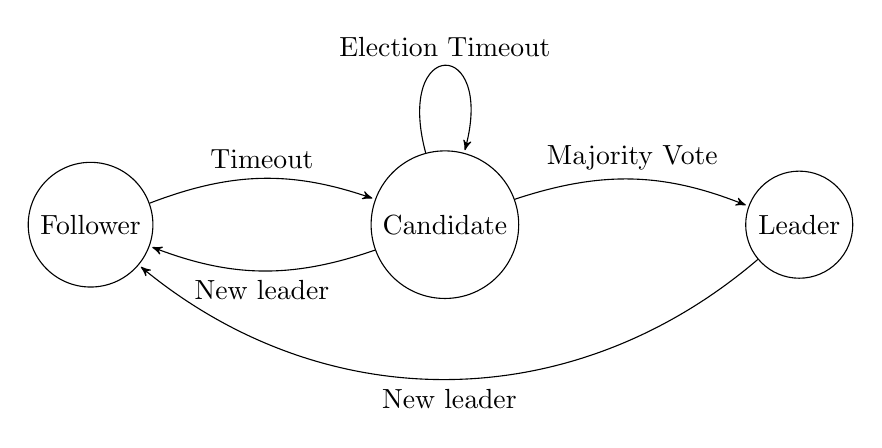
\begin{tikzpicture}[>=stealth',shorten >=1pt,auto,node distance=4.5cm]
  \node[state]  (f)                {Follower};
  \node[state]  (c) [right of=f]  {Candidate};
  \node[state]  (l) [right of=c]  {Leader};

  \path[->]          (f)  edge   [bend left=20]   node {Timeout} (c);
  \path[->]          (c)  edge   [bend left=20]   node {New leader} (f);

  \path[->]          (c)  edge   [bend left=20]   node {Majority Vote} (l);
  \path[->]          (l)  edge   [bend left=40]   node {New leader} (f);
  \path[->] (c) edge [loop above] node {Election Timeout} (c);

\end{tikzpicture}
\end{center}

\section{Spec}

The following implements the skeleton portion of the leader election
protocol:\newline

\begin{tla}
Init ==
    /\ state = [s \in Servers |-> "Follower"]
    /\ messages = {} 
    /\ voted_for = [s \in Servers |-> ""]
    /\ vote_granted = [s \in Servers |-> {}]
    /\ vote_requested = [s \in Servers |-> 0]
    /\ term = [s \in Servers |-> 0]

RequestVoteSet(i) == {
    [fSrc |-> i, fDst |-> s, fType |-> "RequestVoteReq", fTerm |-> term[i]] 
        : s \in Servers \ {i}
}

Campaign(i) == 
    /\ vote_requested[i] = 0
    /\ vote_requested' = [vote_requested EXCEPT ![i] = 1]
    /\ messages' = messages \cup RequestVoteSet(i) 
    /\ UNCHANGED <<state, term, vote_granted, voted_for>>

KeepAliveSet(i) == {
    [fSrc |-> i, fDst |-> s, fType |-> "AppendEntryReq", fTerm |-> term[i]] 
        : s \in Servers \ {i}
}

Leader(i) == 
    /\ state[i] = "Leader"
    /\ messages' = messages \cup KeepAliveSet(i) 
    /\ UNCHANGED <<state, voted_for, term, vote_granted, vote_requested>>

BecomeLeader(i) ==
    /\ Cardinality(vote_granted[i]) > Cardinality(Servers) \div 2
    /\ state' = [state EXCEPT ![i] = "Leader"]
    /\ UNCHANGED <<messages, voted_for, 
        term, vote_granted, vote_requested>>

Candidate(i) == 
    /\ state[i] = "Candidate"
    /\ \/ Campaign(i)
       \/ BecomeLeader(i)
       \/ Timeout(i)

Follower(i) == 
    /\ state[i] = "Follower"
    /\ Timeout(i)

Receive(msg) == 
    \/ /\ msg.fType = "AppendEntryReq"
       /\ AppendEntryReq(msg) 
    \/ /\ msg.fType = "AppendEntryResp"
       /\ AppendEntryResp(msg) 
    \/ /\ msg.fType = "RequestVoteReq"
       /\ RequestVoteReq(msg) 
    \/ /\ msg.fType = "RequestVoteResp"
       /\ RequestVoteResp(msg) 

Next == 
    \/ \E i \in Servers : 
          \/ Leader(i) 
          \/ Candidate(i)
          \/ Follower(i)
    \/ \E msg \in messages : Receive(msg)
\end{tla}
\begin{tlatex}
\@x{ Init \.{\defeq}}%
 \@x{\@s{16.4} \.{\land} state \.{=} [ s \.{\in} Servers
 \.{\mapsto}\@w{Follower} ]}%
\@x{\@s{16.4} \.{\land} messages \.{=} \{ \}}%
 \@x{\@s{16.4} \.{\land} voted\_for \.{=} [ s \.{\in} Servers \.{\mapsto}\@w{}
 ]}%
 \@x{\@s{16.4} \.{\land} vote\_granted \.{=} [ s \.{\in} Servers \.{\mapsto}
 \{ \} ]}%
 \@x{\@s{16.4} \.{\land} vote\_requested \.{=} [ s \.{\in} Servers \.{\mapsto}
 0 ]}%
\@x{\@s{16.4} \.{\land} term \.{=} [ s \.{\in} Servers \.{\mapsto} 0 ]}%
\@pvspace{8.0pt}%
\@x{ RequestVoteSet ( i ) \.{\defeq} \{}%
 \@x{\@s{16.4} [ fSrc \.{\mapsto} i ,\, fDst \.{\mapsto} s ,\, fType
 \.{\mapsto}\@w{RequestVoteReq} ,\, fTerm \.{\mapsto} term [ i ] ]}%
\@x{\@s{28.69} \.{:} s \.{\in} Servers \.{\,\backslash\,} \{ i \}}%
\@x{ \}}%
\@pvspace{8.0pt}%
\@x{ Campaign ( i ) \.{\defeq}}%
\@x{\@s{16.4} \.{\land} vote\_requested [ i ] \.{=} 0}%
 \@x{\@s{16.4} \.{\land} vote\_requested \.{'} \.{=} [ vote\_requested
 {\EXCEPT} {\bang} [ i ] \.{=} 1 ]}%
 \@x{\@s{16.4} \.{\land} messages \.{'} \.{=} messages \.{\cup} RequestVoteSet
 ( i )}%
 \@x{\@s{16.4} \.{\land} {\UNCHANGED} {\langle} state ,\, term ,\,
 vote\_granted ,\, voted\_for {\rangle}}%
\@pvspace{8.0pt}%
\@x{ KeepAliveSet ( i ) \.{\defeq} \{}%
 \@x{\@s{16.4} [ fSrc \.{\mapsto} i ,\, fDst \.{\mapsto} s ,\, fType
 \.{\mapsto}\@w{AppendEntryReq} ,\, fTerm \.{\mapsto} term [ i ] ]}%
\@x{\@s{28.69} \.{:} s \.{\in} Servers \.{\,\backslash\,} \{ i \}}%
\@x{ \}}%
\@pvspace{8.0pt}%
\@x{ Leader ( i ) \.{\defeq}}%
\@x{\@s{16.4} \.{\land} state [ i ] \.{=}\@w{Leader}}%
 \@x{\@s{16.4} \.{\land} messages \.{'} \.{=} messages \.{\cup} KeepAliveSet (
 i )}%
 \@x{\@s{16.4} \.{\land} {\UNCHANGED} {\langle} state ,\, voted\_for ,\, term
 ,\, vote\_granted ,\, vote\_requested {\rangle}}%
\@pvspace{8.0pt}%
\@x{ BecomeLeader ( i ) \.{\defeq}}%
 \@x{\@s{16.4} \.{\land} Cardinality ( vote\_granted [ i ] ) \.{>} Cardinality
 ( Servers ) \.{\div} 2}%
 \@x{\@s{16.4} \.{\land} state \.{'} \.{=} [ state {\EXCEPT} {\bang} [ i ]
 \.{=}\@w{Leader} ]}%
\@x{\@s{16.4} \.{\land} {\UNCHANGED} {\langle} messages ,\, voted\_for ,\,}%
\@x{\@s{20.5} term ,\, vote\_granted ,\, vote\_requested {\rangle}}%
\@pvspace{8.0pt}%
\@x{ Candidate ( i ) \.{\defeq}}%
\@x{\@s{16.4} \.{\land} state [ i ] \.{=}\@w{Candidate}}%
\@x{\@s{16.4} \.{\land} \.{\lor} Campaign ( i )}%
\@x{\@s{16.4} \.{\lor} BecomeLeader ( i )}%
\@x{\@s{16.4} \.{\lor} Timeout ( i )}%
\@pvspace{8.0pt}%
\@x{ Follower ( i ) \.{\defeq}}%
\@x{\@s{16.4} \.{\land} state [ i ] \.{=}\@w{Follower}}%
\@x{\@s{16.4} \.{\land} Timeout ( i )}%
\@pvspace{8.0pt}%
\@x{ Receive ( msg ) \.{\defeq}}%
\@x{\@s{16.4} \.{\lor} \.{\land} msg . fType \.{=}\@w{AppendEntryReq}}%
\@x{\@s{16.4} \.{\land} AppendEntryReq ( msg )}%
\@x{\@s{16.4} \.{\lor} \.{\land} msg . fType \.{=}\@w{AppendEntryResp}}%
\@x{\@s{16.4} \.{\land} AppendEntryResp ( msg )}%
\@x{\@s{16.4} \.{\lor} \.{\land} msg . fType \.{=}\@w{RequestVoteReq}}%
\@x{\@s{16.4} \.{\land} RequestVoteReq ( msg )}%
\@x{\@s{16.4} \.{\lor} \.{\land} msg . fType \.{=}\@w{RequestVoteResp}}%
\@x{\@s{16.4} \.{\land} RequestVoteResp ( msg )}%
\@pvspace{8.0pt}%
\@x{ Next \.{\defeq}}%
\@x{\@s{16.4} \.{\lor} \E\, i \.{\in} Servers \.{:}}%
\@x{\@s{16.4} \.{\lor} Leader ( i )}%
\@x{\@s{16.4} \.{\lor} Candidate ( i )}%
\@x{\@s{16.4} \.{\lor} Follower ( i )}%
\@x{\@s{16.4} \.{\lor} \E\, msg \.{\in} messages \.{:} Receive ( msg )}%
\end{tlatex}

\begin{itemize}
    \item \textit{Next} either picks a server to make progress, or picks a
    message in the message pool to process. Message processing is done by
    \textit{Receive}, handling is state agnostic
    \item \textit{message} is defined to be a set that holds a collection of functions, where 
    each function is a message with source, destination, type, and more specified
    \item \textit{voted\_for} tracks who a given node previously voted for.
    This prevents a node from voting more than once
    \item \textit{vote\_granted} tracks how many votes a candidate has received
    \item \textit{vote\_requested} tracks if a node has already issued a request
    vote to its peers
    \item \textit{Follower} either Receive or Timeout and campaign to be a leader
    \item \textit{Candidate} campaigns to be a leader, and becomes one if it has
    enough vote. Failing to collect enough votes, \textit{Candidate} start a new
    election on a new term. It can also receive a request with a higher term and
    transition to be a \textit{Follower}.
    \item \textit{Leader} will establish its leadership by sending
    \textit{AppepndEntryReq} to all its peers
\end{itemize}

 \textit{Spec} implements four messages AppendEntry request/response, RequestVote
request/response. Handling for all messages is similar in structure. In
this chapter, we will look at \textit{RequestVoteReq} only. Readers are
encouraged to check the remaining definition as an exercise:\newline

\begin{tla}
RequestVoteReq(msg) == 
    LET 
        i == msg.fDst
        j == msg.fSrc
        type == msg.fType
        t == msg.fTerm
    IN 
        \* haven't voted, or whom we voted re-requested
        \/ /\ t = term[i]
           /\ \/ voted_for[i] = j 
              \/ voted_for[i] = ""
           /\ voted_for' = [voted_for EXCEPT ![i] = j]
           /\ messages' = AddMessage([fSrc |-> i, 
                                        fDst |-> j, 
                                        fType |-> "RequestVoteResp",
                                        fTerm |-> t, 
                                        fSuccess |-> 1],
                                        RemoveMessage(msg, messages))
           /\ UNCHANGED <<state, term, vote_granted, 
                vote_requested, establish_leadership >>
        \* already voted for someone else
        \/ /\ t = term[i]
           /\ voted_for[i] # j 
           /\ voted_for[i] # ""
           /\ messages' = AddMessage([fSrc |-> i, 
                                        fDst |-> j, 
                                        fType |-> "RequestVoteResp",
                                        fTerm |-> t, 
                                        fSuccess |-> 0],
                                        RemoveMessage(msg, messages))
            /\ UNCHANGED <<state, voted_for, term, 
                vote_granted, vote_requested, establish_leadership>>
        \/  /\ t < term[i]
            /\ messages' = AddMessage([fSrc |-> i, 
                                        fDst |-> j, 
                                        fType |-> "RequestVoteResp",
                                        fTerm |-> term[i], 
                                        fSuccess |-> 0],
                                        RemoveMessage(msg, messages))
            /\ UNCHANGED <<state, voted_for, term, 
                vote_granted, vote_requested, establish_leadership>>
        \* revert to follower
        \/  /\ t > term[i]
            /\ state' = [state EXCEPT ![i] = "Follower"]
            /\ term' = [term EXCEPT ![i] = t]
            /\ voted_for' = [voted_for EXCEPT ![i] = j]
            /\ vote_granted' = [vote_granted EXCEPT ![i] = {}]
            /\ vote_requested' = [vote_requested EXCEPT ![i] = 0]
            /\ establish_leadership' = [establish_leadership EXCEPT ![i] = 0]
            /\ messages' = AddMessage([fSrc |-> i, 
                                        fDst |-> j, 
                                        fType |-> "RequestVoteResp",
                                        fTerm |-> t, 
                                        fSuccess |-> 1],
                                        RemoveMessage(msg, messages))
\end{tla}
\begin{tlatex}
\@x{ RequestVoteReq ( msg ) \.{\defeq}}%
\@x{\@s{16.4} \.{\LET}}%
\@x{\@s{32.8} i \.{\defeq} msg . fDst}%
\@x{\@s{32.8} j \.{\defeq} msg . fSrc}%
\@x{\@s{32.8} type \.{\defeq} msg . fType}%
\@x{\@s{32.8} t \.{\defeq} msg . fTerm}%
\@x{\@s{16.4} \.{\IN}}%
\@x{\@s{32.8}}%
\@y{%
  haven't voted, or whom we voted re-requested
}%
\@xx{}%
\@x{\@s{32.8} \.{\lor} \.{\land} t \.{=} term [ i ]}%
\@x{\@s{32.8} \.{\land} \.{\lor} voted\_for [ i ] \.{=} j}%
\@x{\@s{32.8} \.{\lor} voted\_for [ i ] \.{=}\@w{}}%
 \@x{\@s{32.8} \.{\land} voted\_for \.{'} \.{=} [ voted\_for {\EXCEPT} {\bang}
 [ i ] \.{=} j ]}%
 \@x{\@s{32.8} \.{\land} messages \.{'} \.{=} AddMessage ( [ fSrc \.{\mapsto}
 i ,\,}%
\@x{\@s{41.0} fDst \.{\mapsto} j ,\,}%
\@x{\@s{41.0} fType \.{\mapsto}\@w{RequestVoteResp} ,\,}%
\@x{\@s{41.0} fTerm \.{\mapsto} t ,\,}%
\@x{\@s{41.0} fSuccess \.{\mapsto} 1 ] ,\,}%
\@x{\@s{41.0} RemoveMessage ( msg ,\, messages ) )}%
 \@x{\@s{32.8} \.{\land} {\UNCHANGED} {\langle} state ,\, term ,\,
 vote\_granted ,\,}%
\@x{\@s{41.0} vote\_requested ,\, establish\_leadership {\rangle}}%
\@x{\@s{32.8}}%
\@y{%
  already voted for someone else
}%
\@xx{}%
\@x{\@s{32.8} \.{\lor} \.{\land} t \.{=} term [ i ]}%
\@x{\@s{32.8} \.{\land} voted\_for [ i ] \.{\neq} j}%
\@x{\@s{32.8} \.{\land} voted\_for [ i ] \.{\neq}\@w{}}%
 \@x{\@s{32.8} \.{\land} messages \.{'} \.{=} AddMessage ( [ fSrc \.{\mapsto}
 i ,\,}%
\@x{\@s{41.0} fDst \.{\mapsto} j ,\,}%
\@x{\@s{41.0} fType \.{\mapsto}\@w{RequestVoteResp} ,\,}%
\@x{\@s{41.0} fTerm \.{\mapsto} t ,\,}%
\@x{\@s{41.0} fSuccess \.{\mapsto} 0 ] ,\,}%
\@x{\@s{41.0} RemoveMessage ( msg ,\, messages ) )}%
 \@x{\@s{36.89} \.{\land} {\UNCHANGED} {\langle} state ,\, voted\_for ,\, term
 ,\,}%
 \@x{\@s{40.99} vote\_granted ,\, vote\_requested ,\, establish\_leadership
 {\rangle}}%
\@x{\@s{32.8} \.{\lor}\@s{4.1} \.{\land} t \.{<} term [ i ]}%
 \@x{\@s{36.89} \.{\land} messages \.{'} \.{=} AddMessage ( [ fSrc \.{\mapsto}
 i ,\,}%
\@x{\@s{40.99} fDst \.{\mapsto} j ,\,}%
\@x{\@s{40.99} fType \.{\mapsto}\@w{RequestVoteResp} ,\,}%
\@x{\@s{40.99} fTerm \.{\mapsto} term [ i ] ,\,}%
\@x{\@s{40.99} fSuccess \.{\mapsto} 0 ] ,\,}%
\@x{\@s{40.99} RemoveMessage ( msg ,\, messages ) )}%
 \@x{\@s{36.89} \.{\land} {\UNCHANGED} {\langle} state ,\, voted\_for ,\, term
 ,\,}%
 \@x{\@s{40.99} vote\_granted ,\, vote\_requested ,\, establish\_leadership
 {\rangle}}%
\@x{\@s{32.8}}%
\@y{%
  revert to follower
}%
\@xx{}%
\@x{\@s{32.8} \.{\lor}\@s{4.1} \.{\land} t \.{>} term [ i ]}%
 \@x{\@s{36.89} \.{\land} state \.{'} \.{=} [ state {\EXCEPT} {\bang} [ i ]
 \.{=}\@w{Follower} ]}%
 \@x{\@s{36.89} \.{\land} term \.{'} \.{=} [ term {\EXCEPT} {\bang} [ i ]
 \.{=} t ]}%
 \@x{\@s{36.89} \.{\land} voted\_for \.{'} \.{=} [ voted\_for {\EXCEPT}
 {\bang} [ i ] \.{=} j ]}%
 \@x{\@s{36.89} \.{\land} vote\_granted \.{'} \.{=} [ vote\_granted {\EXCEPT}
 {\bang} [ i ] \.{=} \{ \} ]}%
 \@x{\@s{36.89} \.{\land} vote\_requested \.{'} \.{=} [ vote\_requested
 {\EXCEPT} {\bang} [ i ] \.{=} 0 ]}%
 \@x{\@s{36.89} \.{\land} establish\_leadership \.{'} \.{=} [
 establish\_leadership {\EXCEPT} {\bang} [ i ] \.{=} 0 ]}%
 \@x{\@s{36.89} \.{\land} messages \.{'} \.{=} AddMessage ( [ fSrc \.{\mapsto}
 i ,\,}%
\@x{\@s{40.99} fDst \.{\mapsto} j ,\,}%
\@x{\@s{40.99} fType \.{\mapsto}\@w{RequestVoteResp} ,\,}%
\@x{\@s{40.99} fTerm \.{\mapsto} t ,\,}%
\@x{\@s{40.99} fSuccess \.{\mapsto} 1 ] ,\,}%
\@x{\@s{40.99} RemoveMessage ( msg ,\, messages ) )}%
\end{tlatex}
\newline

The handling is split into three cases: 
\begin{itemize}
    \item If the received request is on a higher term, the processing node grants a vote and becomes a Follower
    \item If the received request is on a lower term, the processing node ignores the request
    \item If the received request is on the same term, the processing node only grants
    vote if it hasn't voted, or has voted for the same requester prior 
\end{itemize}

\section{Model Reduction}

The model checker will run \textit{Spec} as defined but is unlikely to be
completed in a reasonable amount of time due to exponential state growth. We
need to simplify the model, and careful consideration must go into finding the
right balance between maximizing model correctness and minimizing model checker
runtime.\newline

The main strategy is to \textit{bound} the state graph. The following describes
a set of optimizations implemented for this example.

\subsection{Modeling Messages as a Set}

In the original Raft TLA+ Spec \cite{raft_tla}, messages are modeled as an
\textit{unordered map} to track the count of each message. It is possible for a
sender to repeatedly send the same message (eg. keepalive), and grow the 
message count in an unbounded fashion.\newline

\textit{messages} in this example has been implemented as a set, which
effectively limits the message instance count to one. It is still possible for
messages to grow unboundedly because of the monotonically increasing term value.
Further changes are described below.

\subsection{Limit Term Divergence} 

It is possible for a node to \textit{never} make progress. Such a case can occur
when a node is partitioned off while the rest of the cluster elects a new leader
and moves onto newer terms. Many of the interesting behaviors of Raft are how it
addresses these cases. In a cluster of nodes with mixed terms, the nodes with
older terms will eventually converge onto newer terms when they are contacted by
a new leader. This converging behavior will happen whether the stale node is
either 1 or N terms away from the current leader, and the former is much less
costly to simulate than the latter because of the reduced number of states.\newline

We can include \textit{LimitDivergence} as a conjunction in
\textit{Timeout}:\newline
\begin{tla}
LimitDivergence(i) == 
    LET 
        values == {term[s] : s \in Servers}
        max_v == CHOOSE x \in values : \A y \in values : x >= y
        min_v == CHOOSE x \in values : \A y \in values : x <= y
    IN 
        \/ /\ term[i] # max_v
        \/ /\ term[i] = max_v 
           /\ term[i] - min_v < MaxDiff

Timeout(i) == 
    /\ LimitDivergence(i)
    /\ state' = [state EXCEPT ![i] = "Candidate"]
    /\ voted_for' = [voted_for EXCEPT ![i] = i]             \* voted for myself
    /\ vote_granted' = [vote_granted EXCEPT ![i] = {i}]
    /\ vote_requested' = [vote_requested EXCEPT ![i] = 0]
    /\ term' = [term EXCEPT ![i] = @ + 1]                   \* bump term
    /\ establish_leadership' = [establish_leadership EXCEPT ![i] = 0]
    /\ UNCHANGED <<messages>>
    \* /\ PrintT(state')
\end{tla}
\begin{tlatex}
\@x{ LimitDivergence ( i ) \.{\defeq}}%
\@x{\@s{16.4} \.{\LET}}%
\@x{\@s{32.8} values \.{\defeq} \{ term [ s ] \.{:} s \.{\in} Servers \}}%
 \@x{\@s{32.8} max\_v \.{\defeq} {\CHOOSE} x \.{\in} values \.{:} \A\, y
 \.{\in} values \.{:} x \.{\geq} y}%
 \@x{\@s{32.8} min\_v \.{\defeq} {\CHOOSE} x \.{\in} values \.{:} \A\, y
 \.{\in} values \.{:} x \.{\leq} y}%
\@x{\@s{16.4} \.{\IN}}%
\@x{\@s{32.8} \.{\lor} \.{\land} term [ i ] \.{\neq} max\_v}%
\@x{\@s{32.8} \.{\lor} \.{\land} term [ i ] \.{=} max\_v}%
\@x{\@s{32.8} \.{\land} term [ i ] \.{-} min\_v \.{<} MaxDiff}%
\@pvspace{8.0pt}%
\@x{ Timeout ( i ) \.{\defeq}}%
\@x{\@s{16.4} \.{\land} LimitDivergence ( i )}%
 \@x{\@s{16.4} \.{\land} state \.{'} \.{=} [ state {\EXCEPT} {\bang} [ i ]
 \.{=}\@w{Candidate} ]}%
 \@x{\@s{16.4} \.{\land} voted\_for \.{'} \.{=} [ voted\_for {\EXCEPT} {\bang}
 [ i ] \.{=} i ]\@s{49.19}}%
\@y{%
  voted for myself
}%
\@xx{}%
 \@x{\@s{16.4} \.{\land} vote\_granted \.{'} \.{=} [ vote\_granted {\EXCEPT}
 {\bang} [ i ] \.{=} \{ i \} ]}%
 \@x{\@s{16.4} \.{\land} vote\_requested \.{'} \.{=} [ vote\_requested
 {\EXCEPT} {\bang} [ i ] \.{=} 0 ]}%
 \@x{\@s{16.4} \.{\land} term \.{'} \.{=} [ term {\EXCEPT} {\bang} [ i ] \.{=}
 @ \.{+} 1 ]\@s{49.19}}%
\@y{%
  bump term
}%
\@xx{}%
 \@x{\@s{16.4} \.{\land} establish\_leadership \.{'} \.{=} [
 establish\_leadership {\EXCEPT} {\bang} [ i ] \.{=} 0 ]}%
\@x{\@s{16.4} \.{\land} {\UNCHANGED} {\langle} messages {\rangle}}%
\@x{\@s{16.4}}%
\@y{%
  /\ PrintT(state')
}%
\@xx{}%
\end{tlatex}

\subsection{Normalize Cluster Term}

However, \textit{term} can grow unbounded. A monotonically increasing counter is
what many consensus protocols rely on to represent the latest reality. We want to
\textit{normalize} the range of terms in the cluster so the minimum value resets
back to 0 to bound the state graph. This is a trick described in \cite{finite}.
\\

\begin{tla}
Normalize == 
    LET 
        values == {term[s] : s \in Servers}
        max_v == CHOOSE x \in values : \A y \in values : x >= y
        min_v == CHOOSE x \in values : \A y \in values : x <= y
    IN 
        /\ max_v = MaxTerm
        /\ term' = [s \in Servers |-> term[s] - min_v]
        /\ messages' = {}
        /\ UNCHANGED <<state, voted_for, 
            vote_granted, vote_requested, establish_leadership>>

Next == 
    \/ /\ \A i \in Servers : term[i] # MaxTerm 
       /\ \/ \E i \in Servers : 
                \/ Leader(i) 
                \/ Candidate(i)
                \/ Follower(i)
          \/ \E msg \in messages : Receive(msg)
    \/ /\ \E i \in Servers: term[i] = MaxTerm 
       /\ Normalize
\end{tla}
\begin{tlatex}
\@x{ Normalize \.{\defeq}}%
\@x{\@s{16.4} \.{\LET}}%
\@x{\@s{32.8} values \.{\defeq} \{ term [ s ] \.{:} s \.{\in} Servers \}}%
 \@x{\@s{32.8} max\_v \.{\defeq} {\CHOOSE} x \.{\in} values \.{:} \A\, y
 \.{\in} values \.{:} x \.{\geq} y}%
 \@x{\@s{32.8} min\_v \.{\defeq} {\CHOOSE} x \.{\in} values \.{:} \A\, y
 \.{\in} values \.{:} x \.{\leq} y}%
\@x{\@s{16.4} \.{\IN}}%
\@x{\@s{32.8} \.{\land} max\_v \.{=} MaxTerm}%
 \@x{\@s{32.8} \.{\land} term \.{'} \.{=} [ s \.{\in} Servers \.{\mapsto} term
 [ s ] \.{-} min\_v ]}%
\@x{\@s{32.8} \.{\land} messages \.{'} \.{=} \{ \}}%
\@x{\@s{32.8} \.{\land} {\UNCHANGED} {\langle} state ,\, voted\_for ,\,}%
 \@x{\@s{36.89} vote\_granted ,\, vote\_requested ,\, establish\_leadership
 {\rangle}}%
\@pvspace{8.0pt}%
\@x{ Next \.{\defeq}}%
 \@x{\@s{16.4} \.{\lor} \.{\land} \A\, i \.{\in} Servers \.{:} term [ i ]
 \.{\neq} MaxTerm}%
\@x{\@s{16.4} \.{\land} \.{\lor} \E\, i \.{\in} Servers \.{:}}%
\@x{\@s{16.4} \.{\lor} Leader ( i )}%
\@x{\@s{16.4} \.{\lor} Candidate ( i )}%
\@x{\@s{16.4} \.{\lor} Follower ( i )}%
\@x{\@s{16.4} \.{\lor} \E\, msg \.{\in} messages \.{:} Receive ( msg )}%
 \@x{\@s{16.4} \.{\lor} \.{\land} \E\, i \.{\in} Servers \.{:} term [ i ]
 \.{=} MaxTerm}%
\@x{\@s{16.4} \.{\land} Normalize}%
\end{tlatex}
\newline

The implementation ensures only the state machine only moves forward when none
of the nodes is on \textit{MaxTerm}. If any of the nodes are on \textit{MaxTerm},
the cluster terms are normalized.\newline

Another caveat here is in the initial implementation I didn't update messages.
This led to liveness property violation as the messages had terms disagreeing
with the system state. To simplify \textit{Spec} I simply cleared all messages. This 
indirectly verifies a portion of the packet loss handling in \textit{Spec} as well.

\subsection{Sending Request as a Batch}

The send requests were initially implemented using the existential quantifier. 
This introduces many interleaving states. This was replaced with a universal
quantifier so the set of messages is only sent once. The implementation no
longer tracks if the responses were received since \textit{Spec} should handle
packet loss scenarios as well.\\

\begin{tla}
RequestVoteSet(i) == {
    [fSrc |-> i, fDst |-> s, fType |-> "RequestVoteReq", fTerm |-> term[i]] 
        : s \in Servers \ {i}
}

Campaign(i) == 
    /\ vote_requested[i] = 0
    /\ vote_requested' = [vote_requested EXCEPT ![i] = 1]
    /\ messages' = messages \cup RequestVoteSet(i) 
    /\ UNCHANGED <<state, term, vote_granted, 
        voted_for, establish_leadership>>

KeepAliveSet(i) == {
    [fSrc |-> i, fDst |-> s, fType |-> "AppendEntryReq", fTerm |-> term[i]] 
        : s \in Servers \ {i}
}

Leader(i) == 
    /\ state[i] = "Leader"
    /\ establish_leadership[i] = 0
    /\ establish_leadership' = [establish_leadership EXCEPT ![i] = 1]
    /\ messages' = messages \cup KeepAliveSet(i) 
    /\ UNCHANGED <<state, voted_for, term, vote_granted, vote_requested>>
\end{tla}
\begin{tlatex}
\@x{ RequestVoteSet ( i ) \.{\defeq} \{}%
 \@x{\@s{16.4} [ fSrc \.{\mapsto} i ,\, fDst \.{\mapsto} s ,\, fType
 \.{\mapsto}\@w{RequestVoteReq} ,\, fTerm \.{\mapsto} term [ i ] ]}%
\@x{\@s{28.69} \.{:} s \.{\in} Servers \.{\,\backslash\,} \{ i \}}%
\@x{ \}}%
\@pvspace{8.0pt}%
\@x{ Campaign ( i ) \.{\defeq}}%
\@x{\@s{16.4} \.{\land} vote\_requested [ i ] \.{=} 0}%
 \@x{\@s{16.4} \.{\land} vote\_requested \.{'} \.{=} [ vote\_requested
 {\EXCEPT} {\bang} [ i ] \.{=} 1 ]}%
 \@x{\@s{16.4} \.{\land} messages \.{'} \.{=} messages \.{\cup} RequestVoteSet
 ( i )}%
 \@x{\@s{16.4} \.{\land} {\UNCHANGED} {\langle} state ,\, term ,\,
 vote\_granted ,\,}%
\@x{\@s{20.5} voted\_for ,\, establish\_leadership {\rangle}}%
\@pvspace{8.0pt}%
\@x{ KeepAliveSet ( i ) \.{\defeq} \{}%
 \@x{\@s{16.4} [ fSrc \.{\mapsto} i ,\, fDst \.{\mapsto} s ,\, fType
 \.{\mapsto}\@w{AppendEntryReq} ,\, fTerm \.{\mapsto} term [ i ] ]}%
\@x{\@s{28.69} \.{:} s \.{\in} Servers \.{\,\backslash\,} \{ i \}}%
\@x{ \}}%
\@pvspace{8.0pt}%
\@x{ Leader ( i ) \.{\defeq}}%
\@x{\@s{16.4} \.{\land} state [ i ] \.{=}\@w{Leader}}%
\@x{\@s{16.4} \.{\land} establish\_leadership [ i ] \.{=} 0}%
 \@x{\@s{16.4} \.{\land} establish\_leadership \.{'} \.{=} [
 establish\_leadership {\EXCEPT} {\bang} [ i ] \.{=} 1 ]}%
 \@x{\@s{16.4} \.{\land} messages \.{'} \.{=} messages \.{\cup} KeepAliveSet (
 i )}%
 \@x{\@s{16.4} \.{\land} {\UNCHANGED} {\langle} state ,\, voted\_for ,\, term
 ,\, vote\_granted ,\, vote\_requested {\rangle}}%
\end{tlatex}

\subsection{Prune Messages with Stale Terms}

When a node's term advances, all messages targeted to this node with older terms
are discarded. Keeping messages with stale terms allows the model checker to 
verify the node correctly discards them, but can exponentially grow the state
machine. To simplify the model, we can prune stale messages as we add a new 
message: \newline

\begin{tla}
AddMessage(to_add, msgs) == 
    LET 
        pruned == {msg \in msgs : 
                    ~(msg.fDst = to_add.fDst /\ msg.fTerm < to_add.fTerm)}
    IN
        pruned \cup {to_add}

RemoveMessage(to_remove, msgs) ==
\end{tla}
\begin{tlatex}
\@x{ AddMessage ( to\_add ,\, msgs ) \.{\defeq}}%
\@x{\@s{16.4} \.{\LET}}%
\@x{\@s{32.8} pruned \.{\defeq} \{ msg \.{\in} msgs \.{:}}%
 \@x{\@s{36.89} {\lnot} ( msg . fDst \.{=} to\_add . fDst \.{\land} msg .
 fTerm \.{<} to\_add . fTerm ) \}}%
\@x{\@s{16.4} \.{\IN}}%
\@x{\@s{32.8} pruned \.{\cup} \{ to\_add \}}%
\@pvspace{8.0pt}%
\@x{ RemoveMessage ( to\_remove ,\, msgs ) \.{\defeq}}%
\end{tlatex}

\subsection{Enable Symmetry}

Since the behavior is symmetric between nodes, we can enable symmetry to speed
up model checker runtime:\newline

\begin{tla}
Perms == Permutations(Servers)
\end{tla}
\begin{tlatex}
\@x{ Perms \.{\defeq} Permutations ( Servers )}%
\end{tlatex}

\section{Safety}

One of the goals of the protocol is to ensure the cluster only has one leader.
The clusters can have multiple leaders due to unfavorable network connections. For example, a leader node is partitioned off and a new
leader is elected. However, even when the cluster has multiple leaders, they
\textit{must} be on different terms. The leader with the highest term is
effectively the \textit{true leader}. This invariant can be implemented like
so:\newline

\begin{tla}
LeaderUniqueTerm ==
    \A s1, s2 \in Servers :
        (/\state[s1] = "Leader" 
         /\ state[s2] = "Leader" 
         /\ s1 /= s2)   
            => (term[s1] # term[s2])
\end{tla}
\begin{tlatex}
\@x{ LeaderUniqueTerm \.{\defeq}}%
\@x{\@s{16.4} \A\, s1 ,\, s2 \.{\in} Servers \.{:}}%
\@x{\@s{20.5} ( \.{\land} state [ s1 ] \.{=}\@w{Leader}}%
\@x{\@s{24.6} \.{\land} state [ s2 ] \.{=}\@w{Leader}}%
\@x{\@s{24.6} \.{\land} s1 \.{\neq} s2 )}%
\@x{\@s{24.6} \.{\implies} ( term [ s1 ] \.{\neq} term [ s2 ] )}%
\end{tlatex}
\newline

For every pair of nodes, they cannot both be Leaders and have the same
term.

\section{Liveness}

In any failure recovery scenario, the nodes in the cluster converge to a higher
term value either voluntarily or involuntarily. For example: 
\begin{itemize}
    \item A node timed out and started a new election on a new term 
    \item A partitioned follower receives a heartbeat from a new leader on a new term
    \item A candidate receiving a request vote from another candidate on a higher term
\end{itemize}

In any case, a node's term number always increases. This can be described as below:\newline
\begin{tla}
Converge ==
    \A s \in Servers:
        term[s] = 0 ~> term[s] = MaxTerm - MaxDiff
\end{tla}
\begin{tlatex}
\@x{ Converge \.{\defeq}}%
\@x{\@s{16.4} \A\, s \.{\in} Servers \.{:}}%
 \@x{\@s{20.5} term [ s ] \.{=} 0 \.{\leadsto} term [ s ] \.{=} MaxTerm \.{-}
 MaxDiff}%
\end{tlatex}
\newline

Instead of \textit{MaxTerm}, we use \textit{MaxTerm-MaxDiff} to ensure the
liveness property is always upheld even after \textit{Normalization}. However,
running  \textit{Spec} against TLC now will encounter a set of stuttering issues. We
also need to update the fairness description to ensure all possible actions are
called when the enabling conditions are \textit{eventually always} true:\newline

\begin{tla}
Liveness == 
    /\ \A i \in Servers : 
        /\ WF_vars(Leader(i))
        /\ WF_vars(Candidate(i))
        /\ WF_vars(Follower(i))
    /\ WF_vars(\E msg \in messages : Receive(msg))
\end{tla}
\begin{tlatex}
\@x{ Liveness \.{\defeq}}%
\@x{\@s{16.4} \.{\land} \A\, i \.{\in} Servers \.{:}}%
\@x{\@s{20.5} \.{\land} {\WF}_{ vars} ( Leader ( i ) )}%
\@x{\@s{20.5} \.{\land} {\WF}_{ vars} ( Candidate ( i ) )}%
\@x{\@s{20.5} \.{\land} {\WF}_{ vars} ( Follower ( i ) )}%
 \@x{\@s{16.4} \.{\land} {\WF}_{ vars} ( \E\, msg \.{\in} messages \.{:}
 Receive ( msg ) )}%
\end{tlatex}

% \end{document}


\part{Examples with PlusCal}

PlusCal is a C-like syntax that allows designers to describe their
specifications using a pseudo programming language. An use case for PlusCal is
to specify lockless or wait-free data structures.\\

It is possible to express concurrent data structures in TLA+ native notation. To
express a function that can be concurrently executed, the specification needs to
use a PC-like variable to track the statement a context is currently executing.
This is fairly tedious (and possibly error-prone), making PlusCal a more organic
tool to express these designs. 

% \begin{document}

\chapter{SPSC Lockless Queue}


A single producer single consumer (SPSC) lockless queue is a data exchange queue
between a producer and a consumer. The SPSC lockless queue enables data exchange
between producer and consumer without the use of a lock, allowing both producer
and consumer to make progress in all scenarios.\newline

An example application of an SPSC queue is a data exchange interface between the ASIC
and the CPU in a driver implementation.\newline

A real implementation needs to account for memory ordering effects specific to
the architecture. For example, ARM has a weak memory ordering model where
read/write may appear out-of-order between CPUs. In this chapter, we will assume
\textit{logical} execution order where each command is perceived as issued
sequentially (even across CPUs) to focus the discussion on describing the system
using TLA+.
\newline

\section{Requirement}

The following describes the SPSC queue requirements: 

\begin{itemize}
    \item Two executing context, reader and writer
    \item Writer advances wtpr after writes
    \item Reader advances rtpr after reads
    \item If rtpr equals wptr, queue is empty
    \item If (wtpr + 1) \% N equals rptr, queue is full
\end{itemize}

The following is an example of a SPSC queue:
\begin{center}
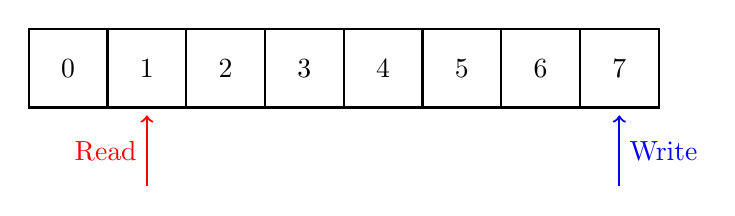
\begin{tikzpicture}
\foreach \i in {0,1,2,3,4,5,6,7} {
    \draw[thick] (\i,0) rectangle (\i+1,1); % Draw each spot in the queue
    \node at (\i+0.5, 0.5) {\i}; % Label each spot
}
\draw[thick, ->, red] (1.5, -1) -- (1.5, -0.1) node[midway, left] {Read};
\draw[thick, ->, blue] (7.5, -1) -- (7.5, -0.1) node[midway, right] {Write};
\end{tikzpicture}
\end{center}

Since the reader and writer execute in different contexts, the instructions in a read
and write can interleave in \textit{any} way imaginable:
\begin{itemize}
    \item Reader empty check can happen just as the writer is writing data
    \item Writer full check can happen just as the reader is reading data
    \item Reading and writing can occur concurrently
\end{itemize}

The key observation is the index held by the write pointer is reserved by the
writer. Similarly, the index held by the read pointer is reserved by the reader. The
only exception is when the read pointer equals to write pointer, then the queue is
empty. Given the possible ways the reader and writer execution can interleave, 
we can use TLA+ to verify the design.

\section{Spec}

TLA+ specification can be written using its native formal specification language,
or a C-like syntax called PlusCal (which transpires down to its native form).
In this example, I chose to implement the specification using PlusCal, since the
content to be verified is pseudo implementation. While it is possible to specify
SPSC in native TLA+, I find the approach more error-prone as each line is
effectively an individual state to be modeled.\newline

The following is a snippet of the \textit{Spec} written in PlusCal:\newline
\begin{ppcal}
procedure reader()
begin
r_chk_empty:        
    if rptr = wptr then 
    r_early_ret:            
        return;
    end if;
r_read_buf:         
    assert buffer[rptr] # 0;
r_cs:               
    buffer[rptr] := 0;
r_upd_rtpr:         
    rptr := (rptr + 1) % N;
    return;
end procedure; 
\end{ppcal}\newline
\begin{tlatex}
\@x{ {\p@procedure} reader ( )}%
\@x{ {\p@begin}}%
\@x{ r\_chk\_empty\@s{.5}\textrm{:}\@s{3}}%
\@x{\@s{16.4} {\p@if} rptr \.{=} wptr {\p@then}}%
\@x{\@s{16.4} r\_early\_ret\@s{.5}\textrm{:}\@s{3}}%
\@x{\@s{32.8} {\p@return} {\p@semicolon}}%
\@x{\@s{16.4} {\p@end} {\p@if} {\p@semicolon}}%
\@x{ r\_read\_buf\@s{.5}\textrm{:}\@s{3}}%
\@x{\@s{16.4} {\p@assert} buffer [ rptr ] \.{\neq} 0 {\p@semicolon}}%
\@x{ r\_cs\@s{.5}\textrm{:}\@s{3}}%
\@x{\@s{16.4} buffer [ rptr ] \.{:=} 0 {\p@semicolon}}%
\@x{ r\_upd\_rtpr\@s{.5}\textrm{:}\@s{3}}%
\@x{\@s{16.4} rptr \.{:=} ( rptr \.{+} 1 ) \.{\%} N {\p@semicolon}}%
\@x{\@s{16.4} {\p@return} {\p@semicolon}}%
\@x{ {\p@end} {\p@procedure} {\p@semicolon}}%
\end{tlatex}

\begin{ppcal}
procedure writer() 
begin
w_chk_full:         
    if (wptr + 1) % N = rptr then 
    w_early_ret:
        return; 
    end if;
w_write_buf:
    assert buffer[wptr] = 0;
w_cs:
    buffer[wptr] := wptr + 1000;
w_upd_wptr:
    wptr := (wptr + 1) % N;
    return;
end procedure; 
\end{ppcal}\newline
\begin{tlatex}
\@x{ {\p@procedure} writer ( )}%
\@x{ {\p@begin}}%
\@x{ w\_chk\_full\@s{.5}\textrm{:}\@s{3}}%
\@x{\@s{16.4} {\p@if} ( wptr \.{+} 1 ) \.{\%} N \.{=} rptr {\p@then}}%
\@x{\@s{16.4} w\_early\_ret\@s{.5}\textrm{:}\@s{3}}%
\@x{\@s{32.8} {\p@return} {\p@semicolon}}%
\@x{\@s{16.4} {\p@end} {\p@if} {\p@semicolon}}%
\@x{ w\_write\_buf\@s{.5}\textrm{:}\@s{3}}%
\@x{\@s{16.4} {\p@assert} buffer [ wptr ] \.{=} 0 {\p@semicolon}}%
\@x{ w\_cs\@s{.5}\textrm{:}\@s{3}}%
\@x{\@s{16.4} buffer [ wptr ] \.{:=} wptr \.{+} 1000 {\p@semicolon}}%
\@x{ w\_upd\_wptr\@s{.5}\textrm{:}\@s{3}}%
\@x{\@s{16.4} wptr \.{:=} ( wptr \.{+} 1 ) \.{\%} N {\p@semicolon}}%
\@x{\@s{16.4} {\p@return} {\p@semicolon}}%
\@x{ {\p@end} {\p@procedure} {\p@semicolon}}%
\end{tlatex}

\section{Safety}

Some safety requirement we can enforce include:\newline

\begin{tla}
MUTEX ==
    ~ ((pc[WRITER] = "w_cs") /\ (pc[READER] = "r_cs") /\ rptr = wptr)

Inv_Basics == 
    /\ ((written \cup writing) \cup unused) = all
    /\ reading \subseteq written                            \* reading is a subset of written
    /\ \A i \in unused : buffer[i] = 0
    /\ \/ Cardinality(to_be_read) + 1 = Cardinality(reading) 
       \/ Cardinality(to_be_read)     = Cardinality(reading) + 1
       \/ Cardinality(to_be_read)     = Cardinality(reading)
    /\ MUTEX
\end{tla}
\begin{tlatex}
\@x{ MUTEX \.{\defeq}}%
 \@x{\@s{16.4} {\lnot} ( ( pc [ WRITER ] \.{=}\@w{w\_cs} ) \.{\land} ( pc [
 READER ] \.{=}\@w{r\_cs} ) \.{\land} rptr \.{=} wptr )}%
\@pvspace{8.0pt}%
\@x{ Inv\_Basics \.{\defeq}}%
 \@x{\@s{16.4} \.{\land} ( ( written \.{\cup} writing ) \.{\cup} unused )
 \.{=} all}%
\@x{\@s{16.4} \.{\land} reading \.{\subseteq} written\@s{110.7}}%
\@y{%
  reading is a subset of written
}%
\@xx{}%
\@x{\@s{16.4} \.{\land} \A\, i \.{\in} unused \.{:} buffer [ i ] \.{=} 0}%
 \@x{\@s{16.4} \.{\land} \.{\lor} Cardinality ( to\_be\_read ) \.{+} 1 \.{=}
 Cardinality ( reading )}%
 \@x{\@s{16.4} \.{\lor} Cardinality ( to\_be\_read )\@s{16.4} \.{=}
 Cardinality ( reading ) \.{+} 1}%
 \@x{\@s{16.4} \.{\lor} Cardinality ( to\_be\_read ) \.{=} Cardinality (
 reading )}%
\@x{\@s{16.4} \.{\land} MUTEX}%
\end{tlatex}
\newline

\section{Liveness}

All indicies are eventually used:

\begin{tla}
    Liveness ==
    \A k \in 0..N-1:
    <>(buffer[k] # 0)
\end{tla}
\begin{tlatex}
\@x{\@s{16.4} Liveness \.{\defeq}}%
\@x{\@s{16.4} \A\, k \.{\in} 0 \.{\dotdot} N \.{-} 1 \.{:}}%
\@x{\@s{16.4} {\Diamond} ( buffer [ k ] \.{\neq} 0 )}%
\end{tlatex}

Unused index 0 becomes used, used index 0 becomes unused.
\begin{tla}
    Liveness2 ==
    /\ (buffer[0] = 0) ~> buffer[0] = 1000
    /\ (buffer[0] = 1000) ~> buffer[0] = 0
\end{tla}
\begin{tlatex}
\@x{\@s{16.4} Liveness2 \.{\defeq}}%
 \@x{\@s{16.4} \.{\land} ( buffer [ 0 ] \.{=} 0 ) \.{\leadsto} buffer [ 0 ]
 \.{=} 1000}%
 \@x{\@s{16.4} \.{\land} ( buffer [ 0 ] \.{=} 1000 ) \.{\leadsto} buffer [ 0 ]
 \.{=} 0}%
\end{tlatex}

% \end{document}

\* Add statements after this line.

SPECIFICATION Spec
\* INVARIANTS TypeOK NotSolved

CONSTANTS 
    N = 4
    READERS = {r0, r1}

INVARIANTS 
    Inv_Basics
    \* Inv_UniqueReaderPointers
    \* Inv_ReadingVsReady
    \* Inv_NonZeroCount
    \* Inv_UniqueReader
    \* Inv_DataValidity
    \* Inv_BufferSlotLifecycle
    \* Inv_ProducerConsumerSeparation
    \* Inv_DataValidity2

PROPERTIES 
    Liveness
    Liveness2

\* SYMMETRY 
\*     Perms


\part{System Modeling}

Specifications described so far have been designed to with finite state space to
allow model checker to explore all states and prove correctness. In this
section, we will relax this and allow infinite state space.\\

This uses TLA+ as a \textit{prototyping} tool. By definition, the model checker
cannot verify infinite sate space. However, for all states it does explore, it
will verify safety properties and highlight all the violations. This enables
designer to quickly iterate on design to flesh out what may or may not work. Per
80/20 rule, the model checker will very quickly identify obvious violations in
the design.\\

Once settled on a design and model checker no longer reports violation in any 
practical amount of time, one can always simplify the specification into finite
space to exhaustively prove correctness. 

% \begin{document}

\usetikzlibrary{arrows.meta} % For double arrows

\chapter{KV Store with Cache}

LRU cache, or least-re cently-used cache, is a finite-sized cache that evicts 
the least-recently-used entry when full. Modern CPU architecture supports
multi-layer cache. Caches closer to the CPU are faster, but also smaller. Cache is 
designed to take advantage of temporal locality, where recently accessed data isgenerally likely to be re-accessed in near future.\\

Caches are also applied more broadly: CDNs (content delivery
networks) are a group of geographically distributed servers close to
users in different parts of the world. Redis is a high-performance in-memory
key-value store, effectively a cache layer without underlying storage. The list of
examples goes on and on.

\section{Design}

In this chapter, we will describe a simple key-value store with a fixed-sized 
write-back LRU cache. The size of the key-value store is assumed unbounded. LRU
cache acts as a fast access buffer until it's full. When it's full, the
least-recently-used entry key-value pair is evicted into the main memory.\\

Similar to a system with a cache, a key may exist in both the cache and memory
with different values. The key-value pair in the cache is assumed up-to-date,
while the key-value pair in memory may be stale. When the key-value pair is
evicted from the cache, the key in memory is synchronized by write-back from
the cache.\\

We will implement three specifications in this chapter: LRU cache, KV store, and
Test, with one building on another. The KV store is implemented using the LRU
cache, and Test verifies the KV stores.

\section{LRU Cache}

LRU cache can be implemented using three data structures: 
\begin{itemize}
    \item Linked list to track key access recency 
    \item Lookup table to track key and recency list iterator 
    \item Lookup table to track the key-value pair
\end{itemize}

% The following represents a visual layout of the three data structure:
\begin{center}
\includegraphics[width=300pt]{lru}
\end{center}

Recency list is a doubly-linked list where the most recently accessed item is at
the tail. On read or write of an existing key, the key to iterator lookup table
is used to identify the key to update. The identified key is then moved to the
tail of the recency list to indicate recent access. Finally, the key-value table
is updated if needed. When inserting a new key-value pair, the head of the
recency list is evicted to make space, if required.\\

When specifying the LRU cache with TLA+, we can omit the key to iterator table
to simplify the specification. Recency list can be implemented as a
\textit{tuple}, and a key-value table as a \textit{function}.\\

\subsection{Spec}

The following implements the LRU put function:\\

\begin{tla}
Put(k, v) == 
    IF k \in DOMAIN lru_kv THEN 
        \* replace
        /\ lru_recency' = Append(SelectSeq(lru_recency, LAMBDA x : x # k), k)
        /\ lru_kv' = [n \in DOMAIN lru_kv |-> IF n = k THEN v ELSE lru_kv[n]]
        /\ UNCHANGED lru_size
    ELSE 
        IF Len(lru_recency) # lru_size THEN 
            \* add 
            /\ lru_recency' = Append(lru_recency, k)
            /\ lru_kv' = [n \in DOMAIN lru_kv \cup {k} |-> n]
            /\ UNCHANGED lru_size
        ELSE 
            \* replace oldest 
            /\ lru_recency' = Append(SelectSeq(lru_recency,         
                                LAMBDA x : x # lru_recency[1]), k)
            /\ lru_kv' = [n \in (DOMAIN lru_kv \cup {k}) \ {lru_recency[1]} |-> 
                            IF n # k THEN lru_kv[n] ELSE v]
            /\ UNCHANGED lru_size
\end{tla}
\begin{tlatex}
\@x{ Put ( k ,\, v ) \.{\defeq}}%
\@x{ {\IF} k \.{\in} {\DOMAIN} lru\_kv \.{\THEN}}%
\@x{\@s{4.1}}%
\@y{%
  replace
}%
\@xx{}%
 \@x{\@s{4.1} \.{\land} lru\_recency \.{'} \.{=} Append ( SelectSeq (
 lru\_recency ,\, {\LAMBDA} x \.{:} x \.{\neq} k ) ,\, k )}%
 \@x{\@s{4.1} \.{\land} lru\_kv \.{'} \.{=} [ n \.{\in} {\DOMAIN} lru\_kv
 \.{\mapsto} {\IF} n \.{=} k \.{\THEN} v \.{\ELSE} lru\_kv [ n ] ]}%
\@x{\@s{4.1} \.{\land} {\UNCHANGED} lru\_size}%
\@x{ \.{\ELSE}}%
\@x{\@s{16.4} {\IF} Len ( lru\_recency ) \.{\neq} lru\_size \.{\THEN}}%
\@x{\@s{20.5}}%
\@y{%
  add 
}%
\@xx{}%
 \@x{\@s{20.5} \.{\land} lru\_recency \.{'} \.{=} Append ( lru\_recency ,\, k
 )}%
 \@x{\@s{20.5} \.{\land} lru\_kv \.{'} \.{=} [ n \.{\in} {\DOMAIN} lru\_kv
 \.{\cup} \{ k \} \.{\mapsto} n ]}%
\@x{\@s{20.5} \.{\land} {\UNCHANGED} lru\_size}%
\@x{\@s{16.4} \.{\ELSE}}%
\@x{\@s{32.8}}%
\@y{%
  replace oldest 
}%
\@xx{}%
 \@x{\@s{32.8} \.{\land} lru\_recency \.{'} \.{=} Append ( SelectSeq (
 lru\_recency ,\,}%
\@x{\@s{41.0} {\LAMBDA} x \.{:} x \.{\neq} lru\_recency [ 1 ] ) ,\, k )}%
 \@x{\@s{32.8} \.{\land} lru\_kv \.{'} \.{=} [ n \.{\in} ( {\DOMAIN} lru\_kv
 \.{\cup} \{ k \} ) \.{\,\backslash\,} \{ lru\_recency [ 1 ] \} \.{\mapsto}}%
\@x{\@s{32.8} {\IF} n \.{\neq} k \.{\THEN} lru\_kv [ n ] \.{\ELSE} v ]}%
\@x{\@s{32.8} \.{\land} {\UNCHANGED} lru\_size}%
\end{tlatex}
\\

When the implementation needs to extract a key and move it to the end, it uses
\textit{SelectSeq} to remove the targeted key and \textit{Append} to append the
key to the end. When updating \textit{lru\_kv}, the keyspace is expanded with
\textit{k}. In the case keyspace is full, then \textit{lru\_recency[1]} (least 
recent entry in LRU) is evicted.

\subsection{Safety}

For safety, we want to ensure values in \textit{lru\_recency} match with keys
in \textit{lru\_function}. Similarly, LRU size cannot exceed \textit{lru\_size}.\\

\begin{tla}
    Consistent ==
    /\ {lru_recency[k] : k \in DOMAIN lru_recency} = DOMAIN lru_kv
    /\ Cardinality(DOMAIN lru_kv) <= lru_size
\end{tla}
\begin{tlatex}
\@x{\@s{16.4} Consistent \.{\defeq}}%
 \@x{\@s{16.4} \.{\land} \{ lru\_recency [ k ] \.{:} k \.{\in} {\DOMAIN}
 lru\_recency \} \.{=} {\DOMAIN} lru\_kv}%
\@x{\@s{16.4} \.{\land} Cardinality ( {\DOMAIN} lru\_kv ) \.{\leq} lru\_size}%
\end{tlatex}

\subsection{Liveness}

There isn't any notable converging property for the LRU cache. Omitted from this chapter. 

\section{KV Store}

The KV store itself is pretty straightforward in design, naively we need a
single \textit{function} to implement a table that holds the key-value pairs.
The slight complexity is integrating LRU into the KV store. This is described in
the \textit{Update} function:\\

\begin{tla}
Update(k, v) == 
    IF LRU!Contains(k) THEN 
         /\ LRU!Put(k, v)
         /\ UNCHANGED kv
         /\ latency' = CACHED
    ELSE \* LRU does not contain k
        /\ IF LRU!IsFull THEN 
                LET 
                    pair == LRU!GetLeastRecent
                    key == CHOOSE only \in DOMAIN pair: TRUE
                    value == pair[key]
                IN 
                    \* Evicted from LRU and write to memory
                    /\ kv' = [x \in DOMAIN kv \cup {key} |-> 
                                IF x = key THEN value ELSE kv[x]]
            ELSE 
                UNCHANGED kv 
        /\ LRU!Put(k, v)
        /\ latency' = EVICT
\end{tla}
\begin{tlatex}
\@x{ Update ( k ,\, v ) \.{\defeq}}%
\@x{\@s{16.4} {\IF} LRU {\bang} Contains ( k ) \.{\THEN}}%
\@x{\@s{24.59} \.{\land} LRU {\bang} Put ( k ,\, v )}%
\@x{\@s{24.59} \.{\land} {\UNCHANGED} kv}%
\@x{\@s{24.59} \.{\land} latency \.{'} \.{=} CACHED}%
\@x{\@s{16.4} \.{\ELSE}}%
\@y{%
  LRU does not contain k
}%
\@xx{}%
\@x{\@s{32.8} \.{\land} {\IF} LRU {\bang} IsFull \.{\THEN}}%
\@x{\@s{41.0} \.{\LET}}%
\@x{\@s{57.4} pair \.{\defeq} LRU {\bang} GetLeastRecent}%
 \@x{\@s{57.4} key \.{\defeq} {\CHOOSE} only \.{\in} {\DOMAIN} pair \.{:}
 {\TRUE}}%
\@x{\@s{57.4} value \.{\defeq} pair [ key ]}%
\@x{\@s{41.0} \.{\IN}}%
\@x{\@s{57.4}}%
\@y{%
  Evicted from LRU and write to memory
}%
\@xx{}%
 \@x{\@s{57.4} \.{\land} kv \.{'} \.{=} [ x \.{\in} {\DOMAIN} kv \.{\cup} \{
 key \} \.{\mapsto}}%
\@x{\@s{57.4} {\IF} x \.{=} key \.{\THEN} value \.{\ELSE} kv [ x ] ]}%
\@x{\@s{36.89} \.{\ELSE}}%
\@x{\@s{53.29} {\UNCHANGED} kv}%
\@x{\@s{32.8} \.{\land} LRU {\bang} Put ( k ,\, v )}%
\@x{\@s{32.8} \.{\land} latency \.{'} \.{=} EVICT}%
\end{tlatex}
\\

If the LRU contains the key (full or not), we simply update the LRU. The LRU will
update its internal recency list. If LRU doesn't contain the key, we have two
possible scenarios. If the LRU is not full, we can simply insert it into the LRU.
If the LRU is full, we need to evict the least recently used key-value pair 
write back to KV store, and insert the new key-value pair into the LRU.
\subsection{Safety}

Omitted.

\subsection{Liveness}

Omitted.

\section{Test}

Putting everything together, we want to characterize the design and
confirm wget get the expected latency improvement. 

\subsection{Spec}

The core of the test is pretty straightforward, we assume the usual 80/20 rule
where 80\% of the traffic are cache hits and 20\% are cache misses. This can be
simulated using the existential qualifier:\\

\begin{tla}
Next ==
    \/ \E p \in 1..10:
        /\  IF p > 2 THEN
                \* cached
                /\ \E k \in DOMAIN lru_kv:
                    /\ KV!Update(k, lru_kv[k])
                    /\ written' = [x \in DOMAIN written \ {k} |-> 
                                    IF x = k THEN k ELSE written[x]]
            ELSE 
                \* cache miss
                \* /\ PrintT(p)
                /\ \E k \in DataSet \ DOMAIN lru_kv:
                    /\ KV!Update(k, k)
                    /\ written' = [x \in DOMAIN written \ {k} |-> 
                                    IF x = k THEN k ELSE written[x]]
\end{tla}
\begin{tlatex}
\@x{ Next \.{\defeq}}%
\@x{\@s{16.4} \.{\lor} \E\, p \.{\in} 1 \.{\dotdot} 10 \.{:}}%
\@x{\@s{20.5} \.{\land}\@s{4.1} {\IF} p \.{>} 2 \.{\THEN}}%
\@x{\@s{28.7}}%
\@y{%
  cached
}%
\@xx{}%
\@x{\@s{28.7} \.{\land} \E\, k \.{\in} {\DOMAIN} lru\_kv \.{:}}%
\@x{\@s{32.8} \.{\land} KV {\bang} Update ( k ,\, lru\_kv [ k ] )}%
 \@x{\@s{32.8} \.{\land} written \.{'} \.{=} [ x \.{\in} {\DOMAIN} written
 \.{\,\backslash\,} \{ k \} \.{\mapsto}}%
\@x{\@s{36.89} {\IF} x \.{=} k \.{\THEN} k \.{\ELSE} written [ x ] ]}%
\@x{\@s{24.6} \.{\ELSE}}%
\@x{\@s{41.0}}%
\@y{%
  cache miss
}%
\@xx{}%
\@x{\@s{41.0}}%
\@y{%
  /\ PrintT(p)
}%
\@xx{}%
 \@x{\@s{41.0} \.{\land} \E\, k \.{\in} DataSet \.{\,\backslash\,} {\DOMAIN}
 lru\_kv \.{:}}%
\@x{\@s{45.1} \.{\land} KV {\bang} Update ( k ,\, k )}%
 \@x{\@s{45.1} \.{\land} written \.{'} \.{=} [ x \.{\in} {\DOMAIN} written
 \.{\,\backslash\,} \{ k \} \.{\mapsto}}%
\@x{\@s{49.19} {\IF} x \.{=} k \.{\THEN} k \.{\ELSE} written [ x ] ]}%
\end{tlatex}
\\

\subsection{Safety}

We want to verify the KV store with cache returns the correct value for 
all the key-value pairs written:\\

\begin{tla}
Consistent == 
    \A k \in DOMAIN written: 
        KV!Read(k) = written[k]
\end{tla}
\begin{tlatex}
\@x{ Consistent \.{\defeq}}%
\@x{\@s{16.4} \A\, k \.{\in} {\DOMAIN} written \.{:}}%
\@x{\@s{20.5} KV {\bang} Read ( k ) \.{=} written [ k ]}%
\end{tlatex}

\subsection{Liveness}

Omitted.

\section{Statistical Sampling}

To collect statistical latency numbers for the design, include the Community
Module CSV and define Safety property:\\

\begin{tla}
CSVFile ==
    "stat.csv"

Stats ==
    /\ CSVWrite("%1$s", <<latency>>, CSVFile)
\end{tla}
\begin{tlatex}
\@x{ CSVFile \.{\defeq}}%
\@x{\@s{16.4}\@w{stat.csv}}%
\@pvspace{8.0pt}%
\@x{ Stats \.{\defeq}}%
 \@x{\@s{16.4} \.{\land} CSVWrite (\@w{\%1\$s} ,\, {\langle} latency {\rangle}
 ,\, CSVFile )}%
\end{tlatex}
\\

The Safety property \textit{Stats} will be triggered in every state, collecting
the latency number in a .csv. To generate the .csv: 

\begin{verbatim}
rm -rf *.csv 
    && java -cp tla2tools.jar tlc2.TLC \
        -generate -note ~/dev/tla/tla/test_kv
\end{verbatim}

The latency numbers have now been collected into stat.csv. Now let us count the
latency numbers:

\begin{verbatim}
cat stat.csv  | grep 10 -ws | wc 
    && cat stat.csv  | grep 100 -ws | wc

  34674   34674  104022
   9239    9239   36956
\end{verbatim}

With a total of 43913 samples, cache hit happens about 78.9\% of the time. This 
closely matches the desired 80\% cache hit defined in the test.

% \end{document}


% \begin{document}

\usetikzlibrary{arrows.meta} % For double arrows

\chapter{Dropbox}

TLA+ is a \textit{thinking tool}. Writing a specification with TLA+ and verify
it against the model checker encourages the designer to exhaustively consider
all corner cases in the design. In this chapter, we will specify a Dropbox-like
service with TLA+ and use the model checker to flesh out the design.\\

\section{Design}

The simplified Dropbox-like service includes a block server that holds physical 
copies of all versions of user files, and a meta server that holds meta data on
all the files and path to the block server. A client contacts both meta and
block server as needed to keep up-to-date. In this design, client attempts to
stay up-to-date on all the file meta, but selectively download the physical
files as needed to save bandwidth.\\

A client can make local changes to a file. The updated file is committed when
the client syncs with meta and block server. The change is then propagated to
the other clients. If multiple clients made changes to the same file, the first
one to upload wins and the other clients need to rebase their changes on top of
latest and attempt to upload again.\\

The system design is visualized below:\\

\begin{center}
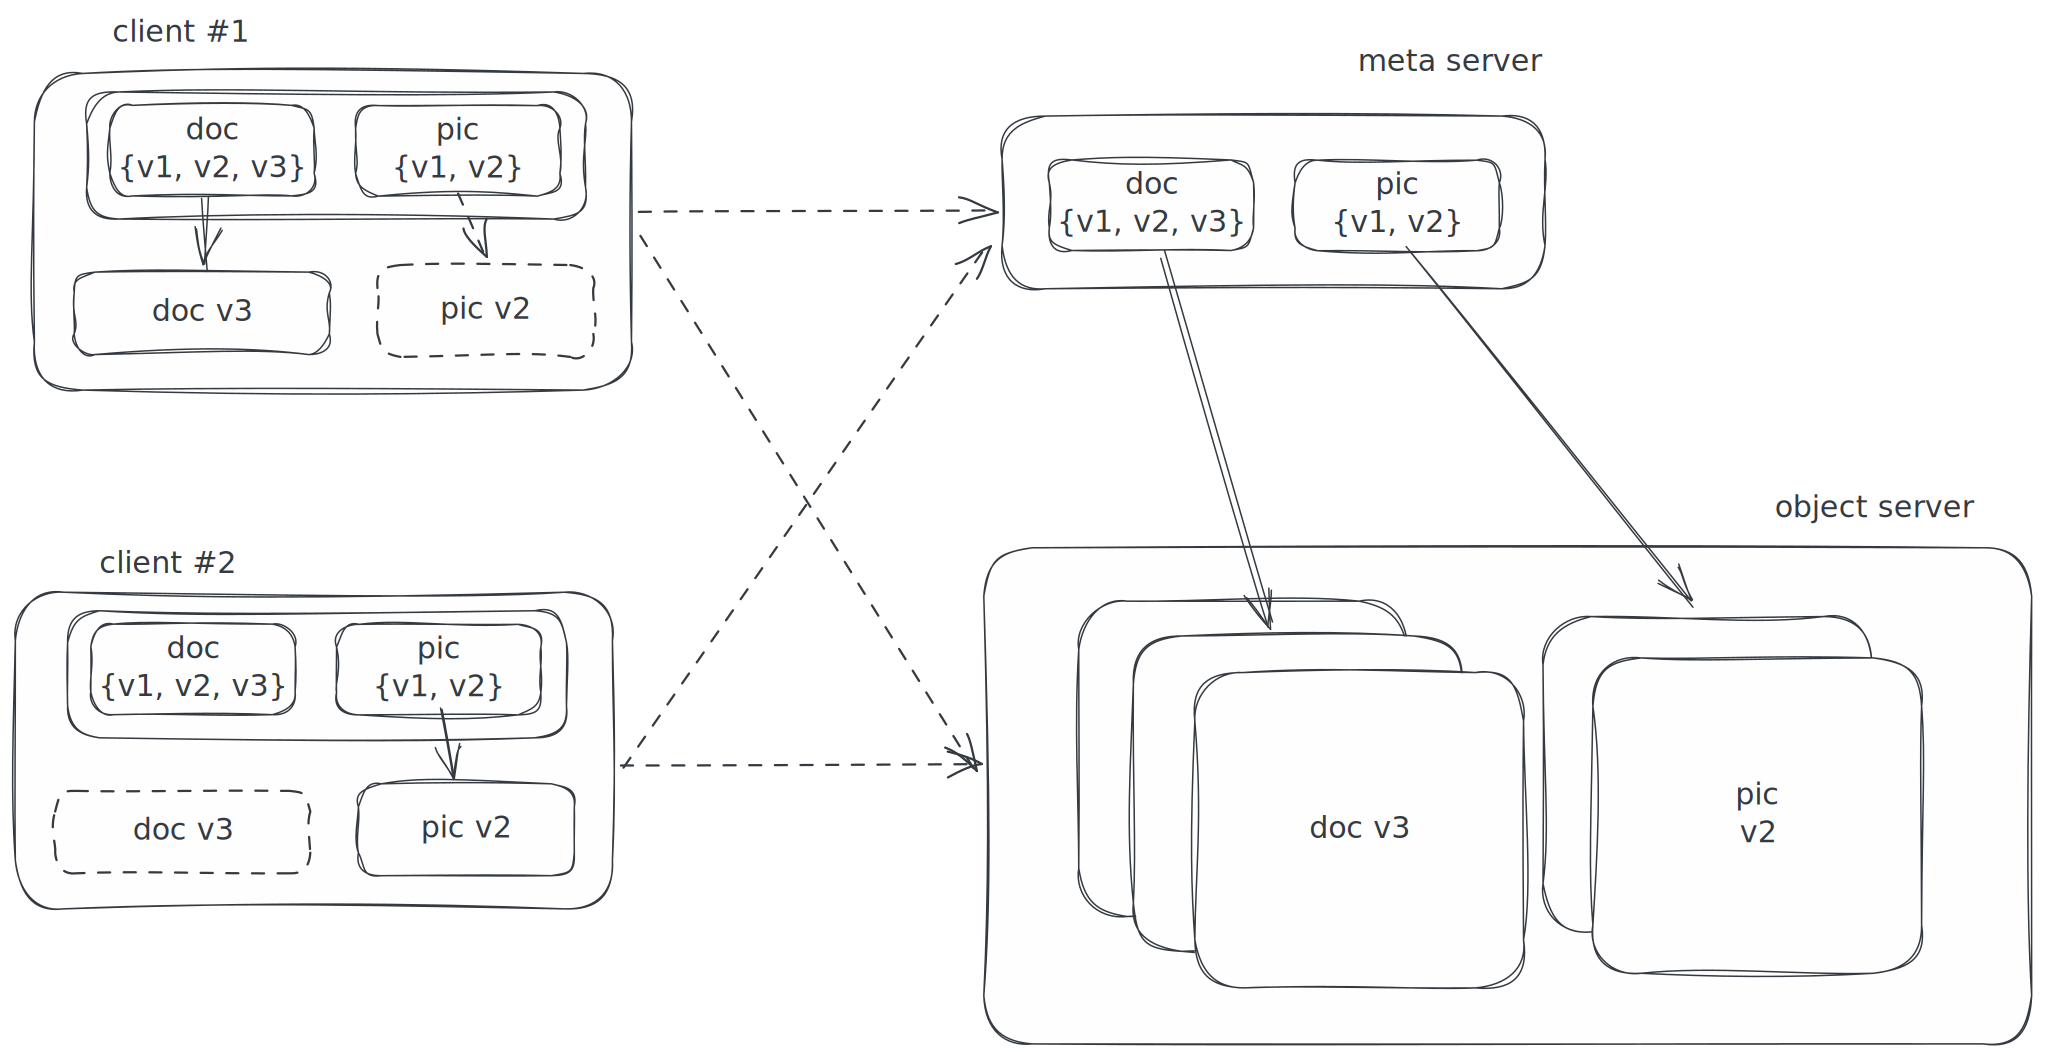
\includegraphics[width=300pt]{dropbox}
\end{center}

\section{Spec}

The following describes the variables used track system state:\\
\begin{tla}
Init ==
    /\ meta_server = [f \in Files |-> {1}]                 
    /\ block_server = [f \in Files |-> <<5>>]
    /\ client_meta = [k \in Clients |-> meta_server]
    /\ client_change = [k \in Clients |-> [f \in Files |-> FALSE]]
    /\ client_block = [k \in Clients |-> <<>>]
\end{tla}
\begin{tlatex}
\@x{ Init \.{\defeq}}%
 \@x{\@s{16.4} \.{\land} meta\_server \.{=} [ f \.{\in} Files \.{\mapsto} \{ 1
 \} ]}%
 \@x{\@s{16.4} \.{\land} block\_server \.{=} [ f \.{\in} Files \.{\mapsto}
 {\langle} 5 {\rangle} ]}%
 \@x{\@s{16.4} \.{\land} client\_meta \.{=} [ k \.{\in} Clients \.{\mapsto}
 meta\_server ]}%
 \@x{\@s{16.4} \.{\land} client\_change \.{=} [ k \.{\in} Clients \.{\mapsto}
 [ f \.{\in} Files \.{\mapsto} {\FALSE} ] ]}%
 \@x{\@s{16.4} \.{\land} client\_block \.{=} [ k \.{\in} Clients \.{\mapsto}
 {\langle} {\rangle} ]}%
\end{tlatex}

\begin{itemize}
    \item \textit{meta\_server} is a lookup table of filename to a set of revisions.
    \item \textit{block\_server} is a lookup table of filename to a list of sizes, ordered by revision.
    \item \textit{client\_meta} represents client's local copy of the file meta.
    \item \textit{client\_block} is client's block storage, only holding version of the file specified by client meta.
    \item \textit{client\_change} is a per client per file lookup tracking if the file has been changed locally.
\end{itemize}

To paint a more concrete picture, this is a snapshot of a state:
\begin{verbatim}
State 94375:
/\ client_block = [c0 |-> [f0 |-> 9, f1 |-> 5], 
                   c1 |-> [f0 |-> 9]]
/\ client_meta = [c0 |-> [f0 |-> 4, f1 |-> 2], 
                  c1 |-> [f0 |-> 2, f1 |-> 1]]
/\ block_server = [f0 |-> <<5, 5, 7>>, f1 |-> <<5, 5>>]
/\ meta_server = [f0 |-> 3, f1 |-> 2]
/\ client_change = [c0 |-> [f0 |-> TRUE, f1 |-> FALSE], 
                    c1 |-> [f0 |-> TRUE, f1 |-> FALSE]]
\end{verbatim}

In this state:
\begin{itemize}
    \item The meta and block server have 2 files: File 0 has 3 revisions and file 1 has 2.
    \item Client 0 downloaded both file 0 and 1.
    \item Client 0 modified file 0 (bumped the revision to 4) but did not modify file 1.
    \item Client 1 meta is out-of-date on both file 0 and 1, but modified file 0.
    \item Client 1 has only downloaded the older revision of file 1, but also modified it.
\end{itemize}

The set of actions allowed is defined below:\\
\begin{tla}
Next ==
    \/ \E k \in Clients: 
        \E f \in Files: 
            \/ SyncMeta(k, f)
            \/ Download(k, f)
            \/ Modify(k, f)
            \/ Upload(k, f)
\end{tla}
\begin{tlatex}
\@x{ Next \.{\defeq}}%
\@x{\@s{16.4} \.{\lor} \E\, k \.{\in} Clients \.{:}}%
\@x{\@s{20.5} \E\, f \.{\in} Files \.{:}}%
\@x{\@s{24.6} \.{\lor} SyncMeta ( k ,\, f )}%
\@x{\@s{24.6} \.{\lor} Download ( k ,\, f )}%
\@x{\@s{24.6} \.{\lor} Modify ( k ,\, f )}%
\@x{\@s{24.6} \.{\lor} Upload ( k ,\, f )}%
\end{tlatex}
\\

In every state, the system can choose to synchronize meta of a file, download a
file, modify a file, or upload a changed file. Some of these operations depend
on each other. For example, a file can only be modified if it has been
downloaded.\\ 

Let us first take a look at \textit{SyncMeta}:\\

\begin{tla}
TailIndex(s) ==
    MaxS(DOMAIN s)

SyncObject(k, f) == 
    IF f \in DOMAIN client_block[k] THEN 
        client_block' 
            = [client_block EXCEPT ![k] 
                = [client_block[k] EXCEPT ![f]
                    = block_server[f][TailIndex(block_server[f])]]]
    ELSE 
        UNCHANGED client_block

SyncMeta(k, f) == 
    IF client_meta[k][f] < meta_server[f]
    \/ (client_meta[k][f] = meta_server[f] /\ client_change[k][f]) THEN 
        \* sync client meta
        /\ client_meta' 
            = [client_meta EXCEPT ![k] 
                = [client_meta[k] EXCEPT ![f]
                    = meta_server[f]]]
        \* sync downloaded file
        /\ SyncObject(k, f)
        /\ client_change' 
            = [client_change EXCEPT ![k] 
                = [client_change[k] EXCEPT ![f] = FALSE]]
        /\ UNCHANGED <<meta_server, block_server>>
    ELSE 
        /\ UNCHANGED vars
\end{tla}
\begin{tlatex}
\@x{ TailIndex ( s ) \.{\defeq}}%
\@x{\@s{16.4} MaxS ( {\DOMAIN} s )}%
\@pvspace{8.0pt}%
\@x{ SyncObject ( k ,\, f ) \.{\defeq}}%
\@x{\@s{16.4} {\IF} f \.{\in} {\DOMAIN} client\_block [ k ] \.{\THEN}}%
\@x{\@s{20.5} client\_block \.{'}}%
\@x{\@s{36.9} \.{=} [ client\_block {\EXCEPT} {\bang} [ k ]}%
\@x{\@s{41.0} \.{=} [ client\_block [ k ] {\EXCEPT} {\bang} [ f ]}%
 \@x{\@s{45.1} \.{=} block\_server [ f ] [ TailIndex ( block\_server [ f ] ) ]
 ] ]}%
\@x{\@s{16.4} \.{\ELSE}}%
\@x{\@s{32.8} {\UNCHANGED} client\_block}%
\@pvspace{8.0pt}%
\@x{ SyncMeta ( k ,\, f ) \.{\defeq}}%
\@x{\@s{16.4} {\IF} client\_meta [ k ] [ f ] \.{<} meta\_server [ f ]}%
 \@x{\@s{16.4} \.{\lor} ( client\_meta [ k ] [ f ] \.{=} meta\_server [ f ]
 \.{\land} client\_change [ k ] [ f ] ) \.{\THEN}}%
\@x{\@s{16.4}}%
\@y{%
  sync client meta
}%
\@xx{}%
\@x{\@s{16.4} \.{\land} client\_meta \.{'}}%
\@x{\@s{20.5} \.{=} [ client\_meta {\EXCEPT} {\bang} [ k ]}%
\@x{\@s{24.6} \.{=} [ client\_meta [ k ] {\EXCEPT} {\bang} [ f ]}%
\@x{\@s{28.7} \.{=} meta\_server [ f ] ] ]}%
\@x{\@s{16.4}}%
\@y{%
  sync downloaded file
}%
\@xx{}%
\@x{\@s{16.4} \.{\land} SyncObject ( k ,\, f )}%
\@x{\@s{16.4} \.{\land} client\_change \.{'}}%
\@x{\@s{20.5} \.{=} [ client\_change {\EXCEPT} {\bang} [ k ]}%
 \@x{\@s{24.6} \.{=} [ client\_change [ k ] {\EXCEPT} {\bang} [ f ] \.{=}
 {\FALSE} ] ]}%
 \@x{\@s{16.4} \.{\land} {\UNCHANGED} {\langle} meta\_server ,\, block\_server
 {\rangle}}%
\@x{\@s{16.4} \.{\ELSE}}%
\@x{\@s{32.8} \.{\land} {\UNCHANGED} vars}%
\end{tlatex}
\\

The client syncs with remote when it is out-of-date. This happens when: remote
has higher revision of the file, or if the client has the same revision of the
file but \textit{local\_change} is set. The current implementation discards and
force update to remote. Practically, the client should rebase and resolve the
conflict.\\

\textit{SyncObject} resets the file to match the remote. This is done by getting
the size of the latest revision for the file. TLA+ doesn't natively provide a
function to get the last element, so \textit{TailIndex} function was added to
facilitate this.\\

The following defines \textit{Download}:\\
\begin{tla}
Download(k, f) == 
    \* only download if meta is up-to-date with no local changes
    /\ client_change[k][f] = FALSE
    /\ client_meta[k][f] = meta_server[f]
    \* Download the latest version
    /\ client_block'
        = [client_block EXCEPT ![k] 
            = [ff \in DOMAIN client_block[k] \cup {f} 
                |-> IF ff # f 
                    THEN client_block[k][ff] 
                    ELSE block_server[f][MaxS(DOMAIN block_server[f])]]]
    /\ UNCHANGED <<client_change, client_meta, meta_server, block_server>>
\end{tla}
\begin{tlatex}
\@x{ Download ( k ,\, f ) \.{\defeq}}%
\@x{\@s{16.4}}%
\@y{%
  only download if meta is up-to-date with no local changes
}%
\@xx{}%
\@x{\@s{16.4} \.{\land} client\_change [ k ] [ f ] \.{=} {\FALSE}}%
\@x{\@s{16.4} \.{\land} client\_meta [ k ] [ f ] \.{=} meta\_server [ f ]}%
\@x{\@s{16.4}}%
\@y{%
  Download the latest version
}%
\@xx{}%
\@x{\@s{16.4} \.{\land} client\_block \.{'}}%
\@x{\@s{20.5} \.{=} [ client\_block {\EXCEPT} {\bang} [ k ]}%
 \@x{\@s{24.6} \.{=} [ ff \.{\in} {\DOMAIN} client\_block [ k ] \.{\cup} \{ f
 \}}%
\@x{\@s{28.7} \.{\mapsto} {\IF} ff \.{\neq} f}%
\@x{\@s{28.7} \.{\THEN} client\_block [ k ] [ ff ]}%
 \@x{\@s{28.7} \.{\ELSE} block\_server [ f ] [ MaxS ( {\DOMAIN} block\_server
 [ f ] ) ] ] ]}%
 \@x{\@s{16.4} \.{\land} {\UNCHANGED} {\langle} client\_change ,\,
 client\_meta ,\, meta\_server ,\, block\_server {\rangle}}%
\end{tlatex}
\\

The client only downloads if file meta is up-to-date and has not been modified
locally.\\

The \textit{Modify} function is defined below:\\

\begin{tla}
Modify(k, f) ==
    /\ client_change[k][f] = FALSE
    \* add new version to client meta
    /\ client_meta' 
        = [client_meta EXCEPT ![k] 
            = [client_meta[k] EXCEPT ![f] 
                = client_meta[k][f] + 1]]
    \* bump client block
    /\ f \in DOMAIN client_block[k]
    /\ \E s \in Sizes: 
       client_block'
        = [client_block EXCEPT ![k] 
            = [client_block[k] EXCEPT ![f] = s]]
    /\ client_change' 
        = [client_change EXCEPT ![k] 
            = [client_change[k] EXCEPT ![f] = TRUE]]
    /\ UNCHANGED <<meta_server, block_server>>
\end{tla}
\begin{tlatex}
\@x{ Modify ( k ,\, f ) \.{\defeq}}%
\@x{\@s{16.4} \.{\land} client\_change [ k ] [ f ] \.{=} {\FALSE}}%
\@x{\@s{16.4}}%
\@y{%
  add new version to client meta
}%
\@xx{}%
\@x{\@s{16.4} \.{\land} client\_meta \.{'}}%
\@x{\@s{20.5} \.{=} [ client\_meta {\EXCEPT} {\bang} [ k ]}%
\@x{\@s{24.6} \.{=} [ client\_meta [ k ] {\EXCEPT} {\bang} [ f ]}%
\@x{\@s{28.7} \.{=} client\_meta [ k ] [ f ] \.{+} 1 ] ]}%
\@x{\@s{16.4}}%
\@y{%
  bump client block
}%
\@xx{}%
\@x{\@s{16.4} \.{\land} f \.{\in} {\DOMAIN} client\_block [ k ]}%
\@x{\@s{16.4} \.{\land} \E\, s \.{\in} Sizes \.{:}}%
\@x{\@s{16.4} client\_block \.{'}}%
\@x{\@s{20.5} \.{=} [ client\_block {\EXCEPT} {\bang} [ k ]}%
 \@x{\@s{24.6} \.{=} [ client\_block [ k ] {\EXCEPT} {\bang} [ f ] \.{=} s ]
 ]}%
\@x{\@s{16.4} \.{\land} client\_change \.{'}}%
\@x{\@s{20.5} \.{=} [ client\_change {\EXCEPT} {\bang} [ k ]}%
 \@x{\@s{24.6} \.{=} [ client\_change [ k ] {\EXCEPT} {\bang} [ f ] \.{=}
 {\TRUE} ] ]}%
 \@x{\@s{16.4} \.{\land} {\UNCHANGED} {\langle} meta\_server ,\, block\_server
 {\rangle}}%
\end{tlatex}
\\

A file can only be modified if it hasn't been. While the client can modify a 
file multiple times, this is modeled as a single revision until the file is
uploaded to remote. A new version of the file is created by bumping the client
local file meta, mark file as changed and assign the file a random size using
existential qualifier.\\

Finally, let's take a look at \textit{Upload}:\\

\begin{tla}
Upload(k, f) == 
    \* client is ahead of the remote with local change
    /\ meta_server[f] < client_meta[k][f]
    /\ client_change[k][f]
    /\ meta_server' 
        = [meta_server EXCEPT ![f] 
            = client_meta[k][f]] \* upload our version
    /\ block_server' = [block_server EXCEPT ![f] 
                        = Append(block_server[f], client_block[k][f])]
    /\ client_change' 
        = [client_change EXCEPT ![k] 
            = [client_change[k] EXCEPT ![f] = FALSE]]
    /\ UNCHANGED <<client_block, client_meta>>
\end{tla}
\begin{tlatex}
\@x{ Upload ( k ,\, f ) \.{\defeq}}%
\@x{\@s{16.4}}%
\@y{%
  client is ahead of the remote with local change
}%
\@xx{}%
\@x{\@s{16.4} \.{\land} meta\_server [ f ] \.{<} client\_meta [ k ] [ f ]}%
\@x{\@s{16.4} \.{\land} client\_change [ k ] [ f ]}%
\@x{\@s{16.4} \.{\land} meta\_server \.{'}}%
\@x{\@s{20.5} \.{=} [ meta\_server {\EXCEPT} {\bang} [ f ]}%
\@x{\@s{24.6} \.{=} client\_meta [ k ] [ f ] ]}%
\@y{%
  upload our version
}%
\@xx{}%
 \@x{\@s{16.4} \.{\land} block\_server \.{'} \.{=} [ block\_server {\EXCEPT}
 {\bang} [ f ]}%
 \@x{\@s{16.4} \.{=} Append ( block\_server [ f ] ,\, client\_block [ k ] [ f
 ] ) ]}%
\@x{\@s{16.4} \.{\land} client\_change \.{'}}%
\@x{\@s{20.5} \.{=} [ client\_change {\EXCEPT} {\bang} [ k ]}%
 \@x{\@s{24.6} \.{=} [ client\_change [ k ] {\EXCEPT} {\bang} [ f ] \.{=}
 {\FALSE} ] ]}%
 \@x{\@s{16.4} \.{\land} {\UNCHANGED} {\langle} client\_block ,\, client\_meta
 {\rangle}}%
\end{tlatex}
\\

Client uploads when it is ahead of remote and has local changes. If the client
is not ahead of remote, remote may have newer version of the file. In such case 
client will call \textit{SyncMeta} to synchronize the remote.

\section{Safety}

\section{Liveness}

% \end{document}



% \begin{document}

\usetikzlibrary{arrows.meta} % For double arrows

\chapter{Decentralized Database}

In the era of big-data today, localized instance of relational database is no
longer enough to hold the volume of data for toady's requirement. Distributed
key-value store has been of a key area of interest in the past few decades. 
Offering such as DynamoDB, Cassandra, Azure Cloud are a few examples of what
industry leaders are offering to address the data problem.\\

Service provided by a distributed key-value store is collectively offered by a
cluster of nodes. The nodes independently restart, update, crash, join or leave 
the cluster, while the service remains uninterrupted (though with possibly
reduced service). As the user base scales, the service must scale accordingly.\\

Two of the key design principles in a distributed data are partition and
replication.\\

A replica group (RG) is a group of nodes that maintain the same set of data.
Nodes in a RG often spans multiple availability zone (AZ) to maximize uptime.
In case of a regional value that wipes out an entire AZ, the other nodes in the
RG can still maintain the service albeit at reduced QoS. The nodes in the RG are
kept in sync using consensus protocol such as Raft. Typically, a write is only
considered complete and ack'd to client once it has been recorded by the
majority of nodes in the RG.

Partition is a way to split the keyspace into slices. When the keyspace is
partitioned, a RG is only responsible for a slice of the keyspace. Bandwidth
demand is also amortized across all RGs. Partition is typically done using 
consistent hashing. Different from traditional hashing, consistent hashing
minimizes data movement when nodes join and leave the clusters. Consistent
hashing will be covered in detail in a later part of the chapter.\\

Some of the early distributed database design requires a centralized server for
meta management (eg. ZooKeeper). In this chapter, we will specify a fully
decentralized key-value store. To simplify the specification, we will assume 
each node itself is a functioning RG with associated reliability property (this
is considered a solved problem with Raft).This chapter will focus on system
behavior correctness as RGs join or leave the cluster and associated data
migration.

\section{Consistent Hashing}

Before we dive into design detail, we must first describe consistent hashing.
With a traditional hashing algorithm, changing the size of the hash space
requires data movement of the entire cluster. This is very undesirable.
Consistent hashing was introduced to minimize data movement, where movement is
only required when adding or removing nodes in the affected range. 

In consistent hashing, the hash space is assumed to be a ring, where the largest
hash value plus one wraps around to the hash of 0. Servers in a consistent
hashing cluster take up different ranges in the ring. For a given request, the
client where the request lands by hashing the request first, then walks the ring
clockwise until it finds a server. \\ 

Assume the following example:

\begin{center}
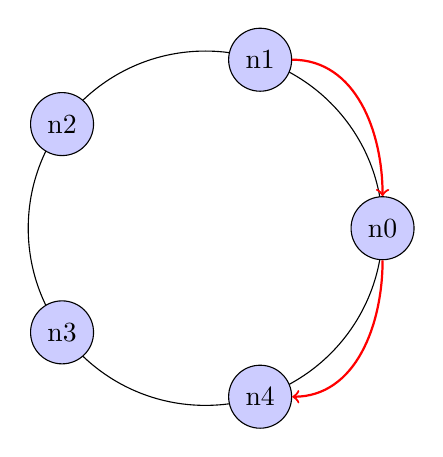
\begin{tikzpicture}[scale=1.5]

    \draw (0,0) circle (1.5cm);

    Draw the nodes on the circle with updated labels
    \foreach \angle/\label in {0/n0, 72/n1, 144/n2, 216/n3, 288/n4} {
        \node[draw, circle, fill=blue!20, minimum size=8mm] at (\angle:1.5cm) (\label) {\label};
    }

    \draw[->, thick, red] (n1) to[out=0, in=90] (n0); % 2 -> 1
    \draw[->, thick, red] (n0) to[out=270, in=0] (n4); % 1 -> 5

\end{tikzpicture}
\end{center}

If the request lands between n1 (exclusive) and n0 (inclusive), the request will
be processed by n0. Similarly, if the request lands between n0 (exclusive) and
n4 (inclusive), the request is to be processed by n4.\\

Assume a case where n4 goes offline: 

\begin{center}
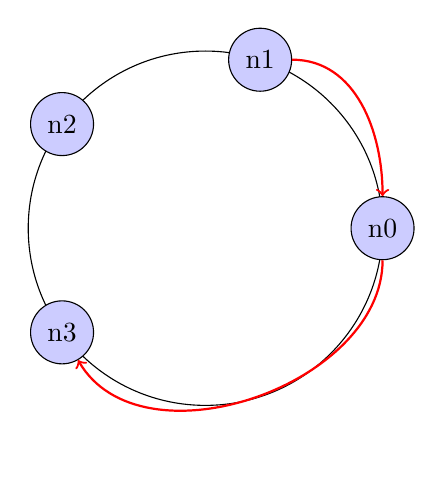
\begin{tikzpicture}[scale=1.5]

    \draw (0,0) circle (1.5cm);

    % Draw the nodes on the circle with updated labels
    \foreach \angle/\label in {0/n0, 72/n1, 144/n2, 216/n3} {
        \node[draw, circle, fill=blue!20, minimum size=8mm] at (\angle:1.5cm) (\label) {\label};
    }

    \draw[->, thick, red] (n1) to[out=0, in=90] (n0); % 2 -> 1
    \draw[->, thick, red] (n0) to[out=270, in=300] (n3); % 1 -> 5

\end{tikzpicture}
\end{center}

In such a case, requests previously processed by n4 will land on n3 instead.
Similarly, if a new node n5 is added:

\begin{center}
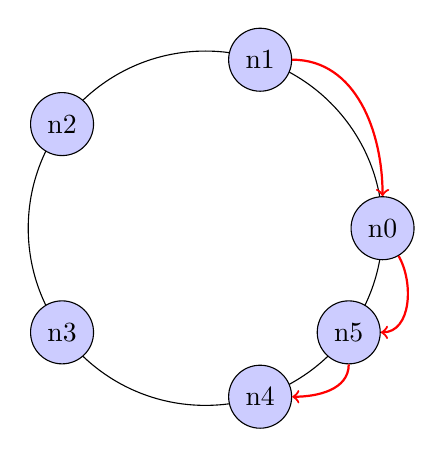
\begin{tikzpicture}[scale=1.5]

    % Draw the circle
    \draw (0,0) circle (1.5cm);

    % Draw the nodes on the circle with updated labels
    \foreach \angle/\label in {0/n0, 72/n1, 144/n2, 216/n3, 288/n4, 324/n5} {
        \node[draw, circle, fill=blue!20, minimum size=8mm] at (\angle:1.5cm) (\label) {\label};
    }

    % Draw arrows
    \draw[->, thick, red] (n1) to[out=0, in=90] (n0); % n1 -> n0
    \draw[->, thick, red] (n0) to[out=300, in=0] (n5); % n0 -> n4
    \draw[->, thick, red] (n5) to[out=270, in=0] (n4); % n0 -> n4

\end{tikzpicture}
\end{center}

Part of what n4 used to service will now be serviced by n5.

\section{Gossip Protocol}

Without a centralized metadata controller, the nodes learn about the peers using
gossip protocol. As a new RG enters the cluster, the design relies on gossip
protocol to spread the information. This is a critical part of the design as
will be described later.

\section{Design}

In our design, a RG can be in one of the following states: Offline, Joining,
Online, Leaving. The service starts with a single RG responsible for the entire
hash space. Since this is the epoch RG, it directly transitions into Online
state and can claim any token on the ring. For simplicity, epoch RG always claim
token 0.\\

The design assumes node failure handling are handled within the RG, the
specification will not model RG crash or restart. 

\subsection{Offline}

RG is offline, no impact to cluster.

\subsection{Joining}

By definition, the goal of adding a RG U into the cluster is to reduce the load
on another RG V. Since RG U is a new member of the cluster, it may not have the
latest cluster topology. Once RG U announces its presence via gossip protocol,
it waits for RG V to reach out.\\

When RG V realizes a new RG can share its burden, RG V will coordinate with RG U
to migrate a subset of its data to RG U (the subset RG U will be responsible
for). Once data migration completes: RG U transitions to Online state and start
servicing request in its range, while RG V rejects request to the range RG U has
taken over. This range update is also reflected in both RG U and V's local ring
cache, and communicated during next round of gossip protocol.

\subsection{Online}

RG is \textit{Online} and responds and records requests in its hash range. 

\subsection{Leaving}

Symmetrically, when a RG U is leaving the cluster, a RG V needs to take over the
range and data RG U is currently responsible for. Similarly to join, RG U 
announce its intent to leave, and wait for RG V to reach out and coordinate the
hand off.\\

Note when RG U is still waiting or in the middle of hand-off, it is still
\textit{Online} and must respond to request, until RV V fully takes over.

% Note this is a \textit{graceful} hand-off. The design assumes any failure
% mitigation is implemented within the RG. 


% Since the entire hash space is always covered by the cluster, a RG U joining 
% the cluster needs to coordinate with another RG V to take over part of RG V's 
% hash space. 
% take over a certain hash range needs to coordinate with RG V which is currently 
% responsible for that 
% cluster needs to coordinate with RG V that is currently responsible for the
% range. When RG U joins the cluster, it will announce its presence via gossip
% protocol. Eventually RG V will realize it can volunteer a part of its range to
% RG U, and 


% In this chapter, we will implement a simple distributed key-value store that
% supports horizontal scale-out. The service provider can add servers into the
% cluster dynamically to reduce the load on individual servers. Similarly, the
% service provider can also remove servers dynamically during off hours to
% minimize server costs.\\

% A new server \textit{K} joining the cluster claims a token \textit{T} on the
% ring. Starting from \textit{T}, walk the ring counter-clockwise to find the
% first neighboring token \textit{P}, \textit{K} owns the range of keys from
% \textit{P} (exclusive) to \textit{T} (inclusive).\\

% The design does not include replication or fault recovery to limit the scope.

\section{Specification}

\textit{Init} is defined below:\\

\begin{tla}
offline == [k \in RGState |-> 
            IF k = "version" THEN 0 
            ELSE IF k = "token" THEN -1
            ELSE IF k = "state" THEN "offline"
            ELSE "unused"]
seed == [k \in RGState |-> 
            IF k = "version" THEN 1 
            ELSE IF k = "token" THEN 0
            ELSE IF k = "state" THEN "online"
            ELSE "unused"]
Init ==
    /\ local_ring = [i \in RGs |-> 
                        [j \in RGs |-> 
                            IF i = SeedRG /\ j = SeedRG
                            THEN seed
                            ELSE offline ]] 
    /\ local_kv = [i \in RGs |-> {}]
    /\ debug_kv = {}
    /\ debug = {}
\end{tla}
\begin{tlatex}
\@x{ offline \.{\defeq} [ k \.{\in} RGState \.{\mapsto}}%
\@x{ {\IF} k \.{=}\@w{version} \.{\THEN} 0}%
\@x{ \.{\ELSE} {\IF} k \.{=}\@w{token} \.{\THEN} \.{-} 1}%
\@x{ \.{\ELSE} {\IF} k \.{=}\@w{state} \.{\THEN}\@w{offline}}%
\@x{ \.{\ELSE}\@w{unused} ]}%
\@x{ seed \.{\defeq} [ k \.{\in} RGState \.{\mapsto}}%
\@x{\@s{4.1} {\IF} k \.{=}\@w{version} \.{\THEN} 1}%
\@x{\@s{4.1} \.{\ELSE} {\IF} k \.{=}\@w{token} \.{\THEN} 0}%
\@x{\@s{4.1} \.{\ELSE} {\IF} k \.{=}\@w{state} \.{\THEN}\@w{online}}%
\@x{\@s{4.1} \.{\ELSE}\@w{unused} ]}%
\@x{ Init \.{\defeq}}%
\@x{\@s{16.4} \.{\land} local\_ring \.{=} [ i \.{\in} RGs \.{\mapsto}}%
\@x{\@s{20.5} [ j \.{\in} RGs \.{\mapsto}}%
\@x{\@s{24.6} {\IF} i \.{=} SeedRG \.{\land} j \.{=} SeedRG}%
\@x{\@s{24.6} \.{\THEN} seed}%
\@x{\@s{24.6} \.{\ELSE} offline ] ]}%
\@x{\@s{16.4} \.{\land} local\_kv \.{=} [ i \.{\in} RGs \.{\mapsto} \{ \} ]}%
\@x{\@s{16.4} \.{\land} debug\_kv \.{=} \{ \}}%
\@x{\@s{16.4} \.{\land} debug \.{=} \{ \}}%
\end{tlatex}
\\

Since RGs operate independently, each RG maintain its view of the ring. This is
tracked by \textit{local\_ring}. The cluster is initialized with a single RG
\textit{SeedRG} with \textit{version} set to 1, \textit{state} set to online and
claims \textit{token} 0 on the ring.\\

\textit{local\_kv} represents the per RG KV store. \textit{debug\_kv} records
what the client has written, this is used to verify consistency of the
distributed database. Finally, a \textit{debug} variable is used to hold a token
in a failure trace.\\

The core set of actions permitted by \textit{Spec} is defined below:\\
\begin{tla}
Next ==
    \/ \E u, v \in RGs:
        /\ Gossip(u, v)
    \/ \E u \in RGs:
        \/ Join(u) 
        \/ JoinMigrate(u)
        \/ Leave(u)
        \/ LeaveMigrate(u)
    \/ \E u \in RGs:
        /\ \E k \in KeySpace:
            /\ k \notin debug_kv
            /\ Write(u, k)
\end{tla}
\begin{tlatex}
\@x{ Next \.{\defeq}}%
\@x{\@s{16.4} \.{\lor} \E\, u ,\, v \.{\in} RGs \.{:}}%
\@x{\@s{20.5} \.{\land} Gossip ( u ,\, v )}%
\@x{\@s{16.4} \.{\lor} \E\, u \.{\in} RGs \.{:}}%
\@x{\@s{20.5} \.{\lor} Join ( u )}%
\@x{\@s{20.5} \.{\lor} JoinMigrate ( u )}%
\@x{\@s{20.5} \.{\lor} Leave ( u )}%
\@x{\@s{20.5} \.{\lor} LeaveMigrate ( u )}%
\@x{\@s{16.4} \.{\lor} \E\, u \.{\in} RGs \.{:}}%
\@x{\@s{20.5} \.{\land} \E\, k \.{\in} KeySpace \.{:}}%
\@x{\@s{24.6} \.{\land} k \.{\notin} debug\_kv}%
\@x{\@s{24.6} \.{\land} Write ( u ,\, k )}%
\end{tlatex}
\\

A RG can \textit{Join} or \textit{Leave} the cluster. However, both are graceful
operations requiring coordination of other nodes from the cluster. To complete
join or leave, another RG has to either offload of take over the range of the
joining or leaving RG.  This is described by \textit{JoinMigrate} and
\textit{LeaveMigrate}. Any pair of nodes can \textit{Gossip} to share their
understanding of the current cluster state. Finally, a client can \textit{Write}
to the database by sending request to a RG.\\

Let us take a look at definition for \textit{Join}:\\
\begin{tla}
ClaimedToken == 
    LET 
        not_offline == {v \in RGs: local_ring[v][v]["state"] # StateOffline}
    IN 
        {local_ring[k][k]["token"]: k \in not_offline}

Join(u) == 
    LET 
        key == CHOOSE any \in KeySpace \ ClaimedToken: TRUE
    IN 
        \* Only ever one node joining at a time
        /\ local_ring[u][u]["state"] = StateOffline
        /\ local_ring' = [local_ring EXCEPT ![u] 
                            = [local_ring[u] EXCEPT ![u]
                                = [k \in RGState |-> 
                                    IF k = "version" THEN local_ring[u][u][k] + 1
                                    ELSE IF k = "token" THEN key
                                    ELSE IF k = "state" THEN StatePrepare
                                    ELSE "unused"]]]
        /\ UNCHANGED <<local_kv, debug_kv, debug>>
\end{tla}
\begin{tlatex}
\@x{ ClaimedToken \.{\defeq}}%
\@x{\@s{16.4} \.{\LET}}%
 \@x{\@s{32.8} not\_offline \.{\defeq} \{ v \.{\in} RGs \.{:} local\_ring [ v
 ] [ v ] [\@w{state} ] \.{\neq} StateOffline \}}%
\@x{\@s{16.4} \.{\IN}}%
 \@x{\@s{32.8} \{ local\_ring [ k ] [ k ] [\@w{token} ] \.{:} k \.{\in}
 not\_offline \}}%
\@pvspace{8.0pt}%
\@x{ Join ( u ) \.{\defeq}}%
\@x{ \.{\LET}}%
 \@x{\@s{16.4} key \.{\defeq} {\CHOOSE} any \.{\in} KeySpace
 \.{\,\backslash\,} ClaimedToken \.{:} {\TRUE}}%
\@x{ \.{\IN}}%
\@x{\@s{16.4}}%
\@y{%
  Only ever one node joining at a time
}%
\@xx{}%
 \@x{\@s{16.4} \.{\land} local\_ring [ u ] [ u ] [\@w{state} ] \.{=}
 StateOffline}%
 \@x{\@s{16.4} \.{\land} local\_ring \.{'} \.{=} [ local\_ring {\EXCEPT}
 {\bang} [ u ]}%
\@x{\@s{24.59} \.{=} [ local\_ring [ u ] {\EXCEPT} {\bang} [ u ]}%
\@x{\@s{28.69} \.{=} [ k \.{\in} RGState \.{\mapsto}}%
 \@x{\@s{32.8} {\IF} k \.{=}\@w{version} \.{\THEN} local\_ring [ u ] [ u ] [ k
 ] \.{+} 1}%
\@x{\@s{32.8} \.{\ELSE} {\IF} k \.{=}\@w{token} \.{\THEN} key}%
\@x{\@s{32.8} \.{\ELSE} {\IF} k \.{=}\@w{state} \.{\THEN} StatePrepare}%
\@x{\@s{32.8} \.{\ELSE}\@w{unused} ] ] ]}%
 \@x{\@s{16.4} \.{\land} {\UNCHANGED} {\langle} local\_kv ,\, debug\_kv ,\,
 debug {\rangle}}%
\end{tlatex}
\\

A RG can only join the cluster if it is currently \textit{Offline}. To join the
cluster, the RG must claim an unclaimed token, enter \textit{Joining} state, and
announces its intent via \textit{Gossip}.\\

The design has taken a shortcut to claim an unclaimed token. In a production
implementation, a newly joined RG will not know which token is unclaimed. Since
the design relies on another RG to \textit{admit} the new RG into the cluster,
in the case of a collision the admitting RG can simply ask the RG that wishes to
join to pick a different token and restart the process. Practically, the hash
space is large enough that collision is unlikely.\\


The following describes \textit{JoinMigrate}:\\
\begin{tla}
RECURSIVE FindPrevToken(_, _)
FindPrevToken(key, ring) ==
    LET 
        condition(v) == ring[v]["state"] # StateOffline 
                    /\ ring[v]["token"] = key
        exists == \E v \in DOMAIN ring: condition(v)
        owner == CHOOSE only \in DOMAIN ring: condition(only)
    IN 
        IF exists THEN
            owner
        ELSE 
            FindPrevToken((key + N - 1) \% N, ring)

JoinMigrate(u) == 
    LET 
        \* previous token
        v == FindPrevToken((local_ring[u][u]["token"] + N - 1) % N, 
                            local_ring[u])
        all_keys == local_kv[u]
        all_online_tokens == AllOnlineTokens(u)
        v_token == local_ring[u][v]["token"]
        v_data == DataSet(v_token, all_online_tokens, all_keys)
        updated == [k \in RGState |-> 
                            IF k = "version" THEN local_ring[u][v]["version"] + 1
                            ELSE IF k = "token" THEN local_ring[u][v]["token"]
                            ELSE IF k = "state" THEN StateOnline
                            ELSE "unused"]
        merged == Merge(u, v)
        local_ring_u == [merged EXCEPT ![u] 
                            = [merged[u] EXCEPT ![v] = updated]]
        local_ring_uv == [local_ring_u EXCEPT ![v] 
                            = [local_ring_u[v] EXCEPT ![v] = updated]]
    IN 
        /\ Cardinality(AllTokens(u)) >= 2
        /\ local_ring[u][u]["state"] = StateOnline
        /\ local_ring[u][v]["state"] = StatePrepare
        /\ Cardinality(all_keys) # 0
        /\ IF v_data # {} THEN 
                /\ local_ring' = local_ring_uv
                /\ local_kv' = [k \in RGs |-> 
                                IF k = u THEN local_kv[k] \ v_data
                                ELSE IF k = v THEN local_kv[k] \cup v_data
                                ELSE local_kv[k]]
            ELSE 
                UNCHANGED <<local_ring, local_kv>>
        /\ UNCHANGED <<debug_kv, debug>>
\end{tla}
\begin{tlatex}
\@x{ {\RECURSIVE} FindPrevToken ( \_ ,\, \_ )}%
\@x{ FindPrevToken ( key ,\, ring ) \.{\defeq}}%
\@x{\@s{16.4} \.{\LET}}%
 \@x{\@s{32.8} condition ( v ) \.{\defeq} ring [ v ] [\@w{state} ] \.{\neq}
 StateOffline}%
\@x{\@s{36.89} \.{\land} ring [ v ] [\@w{token} ] \.{=} key}%
 \@x{\@s{32.8} exists \.{\defeq} \E\, v \.{\in} {\DOMAIN} ring \.{:} condition
 ( v )}%
 \@x{\@s{32.8} owner \.{\defeq} {\CHOOSE} only \.{\in} {\DOMAIN} ring \.{:}
 condition ( only )}%
\@x{\@s{16.4} \.{\IN}}%
\@x{\@s{32.8} {\IF} exists \.{\THEN}}%
\@x{\@s{36.89} owner}%
\@x{\@s{32.8} \.{\ELSE}}%
 \@x{\@s{49.19} FindPrevToken ( ( key \.{+} N \.{-} 1 ) \.{\,\backslash\,}
 \.{\%} N ,\, ring )}%
\@pvspace{8.0pt}%
\@x{ JoinMigrate ( u ) \.{\defeq}}%
\@x{\@s{16.4} \.{\LET}}%
\@x{\@s{32.8}}%
\@y{%
  previous token
}%
\@xx{}%
 \@x{\@s{32.8} v \.{\defeq} FindPrevToken ( ( local\_ring [ u ] [ u ]
 [\@w{token} ] \.{+} N \.{-} 1 ) \.{\%} N ,\,}%
\@x{\@s{32.8} local\_ring [ u ] )}%
\@x{\@s{32.8} all\_keys \.{\defeq} local\_kv [ u ]}%
\@x{\@s{32.8} all\_online\_tokens \.{\defeq} AllOnlineTokens ( u )}%
\@x{\@s{32.8} v\_token \.{\defeq} local\_ring [ u ] [ v ] [\@w{token} ]}%
 \@x{\@s{32.8} v\_data \.{\defeq} DataSet ( v\_token ,\, all\_online\_tokens
 ,\, all\_keys )}%
\@x{\@s{32.8} updated \.{\defeq} [ k \.{\in} RGState \.{\mapsto}}%
 \@x{\@s{41.0} {\IF} k \.{=}\@w{version} \.{\THEN} local\_ring [ u ] [ v ]
 [\@w{version} ] \.{+} 1}%
 \@x{\@s{41.0} \.{\ELSE} {\IF} k \.{=}\@w{token} \.{\THEN} local\_ring [ u ] [
 v ] [\@w{token} ]}%
\@x{\@s{41.0} \.{\ELSE} {\IF} k \.{=}\@w{state} \.{\THEN} StateOnline}%
\@x{\@s{41.0} \.{\ELSE}\@w{unused} ]}%
\@x{\@s{32.8} merged \.{\defeq} Merge ( u ,\, v )}%
\@x{\@s{32.8} local\_ring\_u \.{\defeq} [ merged {\EXCEPT} {\bang} [ u ]}%
\@x{\@s{45.1} \.{=} [ merged [ u ] {\EXCEPT} {\bang} [ v ] \.{=} updated ] ]}%
 \@x{\@s{32.8} local\_ring\_uv \.{\defeq} [ local\_ring\_u {\EXCEPT} {\bang} [
 v ]}%
 \@x{\@s{41.0} \.{=} [ local\_ring\_u [ v ] {\EXCEPT} {\bang} [ v ] \.{=}
 updated ] ]}%
\@x{\@s{16.4} \.{\IN}}%
\@x{\@s{32.8} \.{\land} Cardinality ( AllTokens ( u ) ) \.{\geq} 2}%
 \@x{\@s{32.8} \.{\land} local\_ring [ u ] [ u ] [\@w{state} ] \.{=}
 StateOnline}%
 \@x{\@s{32.8} \.{\land} local\_ring [ u ] [ v ] [\@w{state} ] \.{=}
 StatePrepare}%
\@x{\@s{32.8} \.{\land} Cardinality ( all\_keys ) \.{\neq} 0}%
\@x{\@s{32.8} \.{\land} {\IF} v\_data \.{\neq} \{ \} \.{\THEN}}%
\@x{\@s{41.0} \.{\land} local\_ring \.{'} \.{=} local\_ring\_uv}%
\@x{\@s{41.0} \.{\land} local\_kv \.{'} \.{=} [ k \.{\in} RGs \.{\mapsto}}%
 \@x{\@s{41.0} {\IF} k \.{=} u \.{\THEN} local\_kv [ k ] \.{\,\backslash\,}
 v\_data}%
 \@x{\@s{41.0} \.{\ELSE} {\IF} k \.{=} v \.{\THEN} local\_kv [ k ] \.{\cup}
 v\_data}%
\@x{\@s{41.0} \.{\ELSE} local\_kv [ k ] ]}%
\@x{\@s{36.89} \.{\ELSE}}%
\@x{\@s{53.29} {\UNCHANGED} {\langle} local\_ring ,\, local\_kv {\rangle}}%
\@x{\@s{32.8} \.{\land} {\UNCHANGED} {\langle} debug\_kv ,\, debug {\rangle}}%
\end{tlatex}



% \end{document}


\part{Reference}

\chapter{Fairness and Liveness}

For rigorous definition and proof, please refer to (TODO: citations). This
chapter focus on the application aspect of liveness and fairness and define an elevator 
spec that goes up and down.\newline

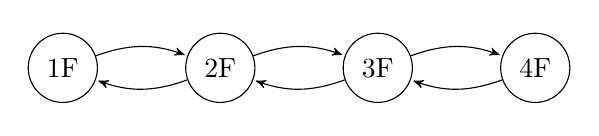
\begin{tikzpicture}[>=stealth',shorten >=1pt,auto,node distance=2cm]
  \node[state]  (q1)                {1F};
  \node[state]  (q2) [right of=q1]  {2F};
  \node[state]  (q3) [right of=q2]  {3F};
  \node[state]  (q4) [right of=q3]  {4F};

  \path[->]          (q1)  edge   [bend left=20]   node {} (q2);
  \path[->]          (q2)  edge   [bend left=20]   node {} (q1);

  \path[->]          (q2)  edge   [bend left=20]   node {} (q3);
  \path[->]          (q3)  edge   [bend left=20]   node {} (q2);

  \path[->]          (q3)  edge   [bend left=20]   node {} (q4);
  \path[->]          (q4)  edge   [bend left=20]   node {} (q3);

\end{tikzpicture}

\section{Liveness}

Consider the following elevator \textit{Spec}:
\begin{tla}
--------------------------- MODULE elevator ----------------------------
EXTENDS Integers
VARIABLES a
vars == <<a>>
TOP     == 4
BOTTOM  == 1
Init ==
    /\ a = BOTTOM
Up == 
    /\ a # TOP
    /\ a' = a + 1
Down == 
    /\ a # BOTTOM
    /\ a' = a - 1
Spec ==
  /\ Init
  /\ [][Up \/ Down]_a
=============================================================================
\end{tla}
\begin{tlatex}
\@x{}\moduleLeftDash\@xx{ {\MODULE} elevator}\moduleRightDash\@xx{}%
\@x{ {\EXTENDS} Integers}%
\@x{ {\VARIABLES} a}%
\@x{ vars \.{\defeq} {\langle} a {\rangle}}%
\@x{ TOP\@s{28.75} \.{\defeq} 4}%
\@x{ BOTTOM\@s{4.10} \.{\defeq} 1}%
\@x{ Init \.{\defeq}}%
\@x{\@s{16.4} \.{\land} a \.{=} BOTTOM}%
\@x{ Up \.{\defeq}}%
\@x{\@s{17.27} \.{\land} a \.{\neq} TOP}%
\@x{\@s{17.27} \.{\land} a \.{'} \.{=} a \.{+} 1}%
\@x{ Down \.{\defeq}}%
\@x{\@s{16.4} \.{\land} a \.{\neq} BOTTOM}%
\@x{\@s{16.4} \.{\land} a \.{'} \.{=} a \.{-} 1}%
\@x{ Spec \.{\defeq}}%
\@x{\@s{8.2} \.{\land}\@s{0.16} Init}%
\@x{\@s{8.2} \.{\land}\@s{0.16} {\Box} [ Up \.{\lor} Down ]_{ a}}%
\@x{}\bottombar\@xx{}%
\end{tlatex}

The building has a set of floors and the elevator can go either up or down. The
elevator keeps going up until it's the top floor, or keep going down until it's
the bottom floor. TLC will pass the \textit{Spec} as is.\newline

Let's introduce a liveness property. The elevator should always at least go 
to the second floor:\newline
\begin{tla}
Liveness == 
    /\ a = 1 ~> a = 2
\end{tla}
\begin{tlatex}
\@x{ Liveness \.{\defeq}}%
\@x{\@s{16.4} \.{\land} a \.{=} 1 \.{\leadsto} a \.{=} 2}%
\end{tlatex}
\newline

Running the \textit{Spec} against TLC will report a violation:

\begin{verbatim}
Error: Temporal properties were violated.
Error: The following behavior constitutes a counter-example:
State 1: <Initial predicate>
a = 1
State 2: Stuttering
\end{verbatim}

Since the \textit{Spec} permits \textit{suttering}, the state machine is allowed
to perpetually stay on 1F and \textit{never} go to 2F. This can be fixed by
introducing fairness description.

\section{Weak Fairness}

Weak fairness is defined as:\newline
\begin{equation} 
\Diamond\Box(ENABLED\langle A \rangle _v) \implies \Box\Diamond\langle A \rangle _v
\end{equation}
$ENABLED\langle A \rangle$ represents \textit{conditions required} for action A.
The above translates to: if conditions required for action A to occur is
\textit{eventually always} true, then action A will \textit{always eventually}
happen.\newline 

Without weak fairness defined, the elevator may \textit{stutter} at 1F and
never go to 2F. Weak fairness states that if the conditions of an action is
\textit{eventually always} true (ie. elevator decides to stay on 1F but 
\textit{can} go up), the elevator \textit{always eventually} go up.\newline

\begin{tla}
Spec ==
  /\ Init
  /\ [][Down \/ Up]_a
  /\ WF_a(Down)
  /\ WF_a(Up)
\end{tla}
\begin{tlatex}
\@x{ Spec \.{\defeq}}%
\@x{\@s{8.2} \.{\land}\@s{0.16} Init}%
\@x{\@s{8.2} \.{\land}\@s{0.16} {\Box} [ Down \.{\lor} Up ]_{ a}}%
\@x{\@s{8.2} \.{\land}\@s{0.16} {\WF}_{ a} ( Down )}%
\@x{\@s{8.2} \.{\land}\@s{0.16} {\WF}_{ a} ( Up )}%
\end{tlatex}
\newline

Running the spec against TLC passes again. What if we want to verify the
elevator eventually always goes to the top, not just to 2F? Let's modify the
Liveness property again:\newline
\begin{tla}
Liveness == 
    /\ a = BOTTOM ~> a = TOP
\end{tla}
\begin{tlatex}
\@x{ Liveness \.{\defeq}}%
\@x{\@s{16.4} \.{\land} a \.{=} BOTTOM \.{\leadsto} a \.{=} TOP}%
\end{tlatex}
\newline

TLC now reports the following violation: 
\begin{verbatim}
Error: Temporal properties were violated.
Error: The following behavior constitutes a counter-example:
State 1: <Initial predicate>
a = 1
State 2: <Up line 10, col 5 to line 11, col 17 of module elevator>
a = 2
Back to state 1: <Down line 13, col 5 to line 14, col 17 of module elevator>
\end{verbatim}

TLC identified a case where the elevator is perpetually stuck going between 1F
and 2F, but never go to 3F. Weak fairness is no longer enough, because the the
elevator is not stuck on 2F repeatedly, but stuck going between 1F and 2F. This
is where we need strong fairness.

\section{Strong Fairness}

Strong fairness is defined as:\newline
\begin{equation} 
\Box\Diamond(ENABLED\langle A \rangle _v) \implies \Box\Diamond\langle A \rangle _v
\end{equation}
The difference between weak and strong fairness is the \textit{eventually
always} vs. \textit{always eventually}. \newline 

In weak fairness, once the state machine is stuck in a state forever, the state
machine always transition to a possible next state permitted by the
\textit{Spec} (eg. if the elevator is stuck on 1F but can go to 2F, it will).
With strong fairness, the elevator doesn't need to be stuck on 2F to go to 3F.
If the elevator \textit{always eventually} makes it to 2F, it \textit{always
eventually} go to 3F.\newline 

Intuitively we are tempted to enable strong fairness like so: \newline
\begin{tla}
Spec ==
  /\ Init
  /\ [][Up \/ Down]_a
  /\ WF_a(Down)
  /\ SF_a(UP)
\end{tla}
\begin{tlatex}
\@x{ Spec \.{\defeq}}%
\@x{\@s{8.2} \.{\land}\@s{0.16} Init}%
\@x{\@s{8.2} \.{\land}\@s{0.16} {\Box} [ Up \.{\lor} Down ]_{ a}}%
\@x{\@s{8.2} \.{\land}\@s{0.16} {\WF}_{ a} ( Down )}%
\@x{\@s{8.2} \.{\land}\@s{0.16} {\SF}_{ a} ( UP )}%
\end{tlatex}
\newline 

However, TLC \textit{still} reports the same violation. What's going on?\newline

If we take a closer look at the enabling condition for \textit{Up}, it only
requires current floor to be not the \textit{top floor}. When the elevator is
stuck in a loop going Up and Down between 1F and 2F indefinitely, strong
fairness for Up is \textit{already satisfied}. What we really want is strong
fairness on \textit{Up} for \textit{every floor}, instead of \textit{any floor
except top floor}. So if elevator makes to 2F once, it will \textit{always
eventaully} go to 3F. If elevator makes to 3F once, it will \textit{always
eventaully} go to 4F, so on and so forth. The following is the change
required:\newline

\begin{tla}
Spec ==
  /\ Init
  /\ [][Up \/ Down]_a
  /\ WF_a(Down)
  /\ \A f \in BOTTOM..TOP-1: 
    /\ WF_a(Up /\ f = a)
\end{tla}
\begin{tlatex}
\@x{ Spec \.{\defeq}}%
\@x{\@s{8.2} \.{\land}\@s{0.16} Init}%
\@x{\@s{8.2} \.{\land}\@s{0.16} {\Box} [ Up \.{\lor} Down ]_{ a}}%
\@x{\@s{8.2} \.{\land}\@s{0.16} {\WF}_{ a} ( Down )}%
 \@x{\@s{8.2} \.{\land}\@s{0.16} \A\, f \.{\in} BOTTOM \.{\dotdot} TOP \.{-} 1
 \.{:}}%
\@x{\@s{16.4} \.{\land} {\WF}_{ a} ( Up \.{\land} f \.{=} a )}%
\end{tlatex}
\newline

Once again with this change TLC will pass.

% \begin{document}

\chapter{Liveness}
\label{chap:liveness}

In this chapter we will go through a very simple state machine to demonstare
liveness properties. Assume a simple three state system:\newline

\begin{center}
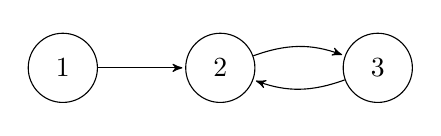
\begin{tikzpicture}[>=stealth',shorten >=1pt,auto,node distance=2cm]
  \node[state]  (q1)                {1};
  \node[state]  (q2) [right of=q1]  {2};
  \node[state]  (q3) [right of=q2]  {3};

  \path[->]          (q1)  edge   []   node {} (q2);
%   \path[->]          (q2)  edge   [bend left=20]   node {} (q1);

  \path[->]          (q2)  edge   [bend left=20]   node {} (q3);
  \path[->]          (q3)  edge   [bend left=20]   node {} (q2);
\end{tikzpicture}
\end{center}

This can be described by the following Spec:\newline

\begin{tla}
--------------------------- MODULE liveness ----------------------------
EXTENDS Naturals
VARIABLES counter 
vars == <<counter>>

EventuallyAlways == <>[](counter = 3)
AlwaysEventually == []<>(counter = 3)

Init ==
    /\ counter = 0

Inc == 
    /\ counter' = counter + 1

Dec == 
    /\ counter' = counter - 1

Next ==
    \/ /\ counter # 3
       /\ Inc
    \/ /\ counter = 3
       /\ Dec

Spec ==
  /\ Init
  /\ [][Next]_vars
  /\ WF_vars(Next)
=============================================================================
\end{tla}
\begin{tlatex}
\@x{}\moduleLeftDash\@xx{ {\MODULE} liveness}\moduleRightDash\@xx{}%
\@x{ {\EXTENDS} Naturals}%
\@x{ {\VARIABLES} counter}%
\@x{ vars \.{\defeq} {\langle} counter {\rangle}}%
\@pvspace{8.0pt}%
\@x{ EventuallyAlways \.{\defeq} {\Diamond} {\Box} ( counter \.{=} 3 )}%
\@x{ AlwaysEventually \.{\defeq} {\Box} {\Diamond} ( counter \.{=} 3 )}%
\@pvspace{8.0pt}%
\@x{ Init \.{\defeq}}%
\@x{\@s{16.4} \.{\land} counter \.{=} 0}%
\@pvspace{8.0pt}%
\@x{ Inc \.{\defeq}}%
\@x{ \.{\land} counter \.{'} \.{=} counter \.{+} 1}%
\@pvspace{8.0pt}%
\@x{ Dec \.{\defeq}}%
\@x{ \.{\land} counter \.{'} \.{=} counter \.{-} 1}%
\@pvspace{8.0pt}%
\@x{ Next \.{\defeq}}%
\@x{\@s{16.4} \.{\lor} \.{\land} counter \.{\neq} 3}%
\@x{\@s{16.4} \.{\land} Inc}%
\@x{\@s{16.4} \.{\lor} \.{\land} counter \.{=} 3}%
\@x{\@s{16.4} \.{\land} Dec}%
\@pvspace{8.0pt}%
\@x{ Spec \.{\defeq}}%
\@x{\@s{8.2} \.{\land} Init}%
\@x{\@s{8.2} \.{\land} {\Box} [ Next ]_{ vars}}%
\@x{\@s{8.2} \.{\land} {\WF}_{ vars} ( Next )}%
\@x{}\bottombar\@xx{}%
\end{tlatex}

Note the required fairness description in the spec. Without fairness the spec is
allowed to stuttering and model checker cannot verify liveness properties. 

\section{Always Eventually}

We want to verify the system always eventually makes it to state 3. This can be
described by the following liveness property:\newline

\begin{tla}
    AlwaysEventually == []<>(counter = 3)
\end{tla}
\begin{tlatex}
 \@x{\@s{16.4} AlwaysEventually \.{\defeq} {\Box} {\Diamond} ( counter \.{=} 3
 )}%
\end{tlatex}
\newline

Once the system makes it to state 3, the system is stuck in a loop transitioning
state 2 and 3. It doesn't \textit{remain} in state 3, but it does \textit{always
eventually} make it to state 3. The system as described fulfills this liveness
property.

\section{Eventually Always}

However, the system does not \textit{eventually always} stay in state 3, because
the system toggles between state 2 and 3. This is described by the following
liveness property: 

\begin{tla}
    AlwaysEventually == []<>(counter = 3)
\end{tla}
\begin{tlatex}
 \@x{\@s{16.4} AlwaysEventually \.{\defeq} {\Box} {\Diamond} ( counter \.{=} 3
 )}%
\end{tlatex}

To satisfy this liveness property, we will need to remove the transition from 3
to 2: 
\begin{tla}
Next ==
    \/ /\ counter # 3
       /\ Inc
\end{tla}


\section{Leads To}

% \end{document}


\chapter{General Guideline}

\section{Model Checker Debug}

Debugging in TLC is a bit different than debugging with normal programs. A step
in the model checker is really a state transition. Even if the model cheker
completes, it's still worthwhile dump and audit the states just to make sure the
Spec is defined correctly.

\begin{verbatim}
tlc elevator -dump out > /dev/null && cat out.dump | head -n5
State 1:
a = 1
State 2:
a = 2
\end{verbatim}

You may want to grep the output to look for state being set to certain value to 
confirm the Spec is working as intended.

\subsection{Dead Lock}

Deadlock typically happens when the model checker ran out of things to do. This
is typically a result of an incomplete Spec definition, where certain edge cases
were not accounted for. The model checker typically provides a fairly
comprehensive backtrace leading up to the dead lock to simplify debug.

\subsection{Live Lock}

Livelock happens when the model checker identifies a case where the liveness
property is violated. An example is the elevator stuck going between two floors 
instead of keep going to the top floor, or the system is stuck dropping and
retransmit the same packet.\newline 

These are typically fixed by providing additional fairness description to the
Spec, telling the model checker how continue in the case of a live lock.\newline 

For a detail fairness description please refer to Chapter~\ref{chap:fairness}.

\section{Model Refinement}

This is, in some sense, the \textit{art} associated with writing model checker
verifiable TLA+ spec. Model checking is only valuable if it can be verified
within a reasonable amount of time. Since the model complexity grows
exponentially, there's little value in attempting to hyper-optimize the details.
Designer should focus on optimizing the broad stroke, such as removing features 
that are harder to get wrong, and focus the model on the bits that have the
highest return on investment.\newline

One useful way of trimming out low value portion of the Spec is to audit the
state dump. Even in the case of a non-terminating run, a partial state dump may
help identify low value details that can be removed from the Spec.\newline

One key value of TLA+ is it highlights all the corner cases in the system. Even
if designer end up simplifying the Spec, it still likely highlights certain
condition the designer was previously unaware of.\newline

As a broad stroke principle: when the Spec has millions or higher more states,
it is unlikely to terminate within a few seconds. From first principles if a
designer can find one failure case in a million states, designer can also likely
simplify the model to reproduce the failure in much fewer states.





% \begin{document}

\chapter{Data Structure}

TLA+ fundamentally supports two different data structures: \textit{Set} and
\textit{Function}. All other data structures are built on-top of these two
primitives.

\section{Set}

Set is an unordered set where every element in the set is unique. TLA+ Set
includes common set operation including union, intersection, membership check,
and more. Set is declared using the squiggly operator, \textit{\{\}}.\\

The following defines a few Set usage examples:\\

\begin{tla}
a == {0, 1, 2}
b == {2, 3, 4}

\* \{0, 1, 2, 3, 4\}
c == a \union b         

\* \{2\}
d == a \intersect b     

\* \{0, 1, 3, 4\} - c substracts d
k == c \ d             
\end{tla}
\begin{tlatex}
\@x{ a \.{\defeq} \{ 0 ,\, 1 ,\, 2 \}}%
\@x{ b \.{\defeq} \{ 2 ,\, 3 ,\, 4 \}}%
\@pvspace{8.0pt}%
\@x{}%
\@y{%
  \{0, 1, 2, 3, 4\}
}%
\@xx{}%
\@x{ c \.{\defeq} a \.{\cup} b}%
\@pvspace{8.0pt}%
\@x{}%
\@y{%
  \{2\}
}%
\@xx{}%
\@x{ d \.{\defeq} a \.{\cap} b}%
\@pvspace{8.0pt}%
\@x{}%
\@y{%
  \{0, 1, 3, 4\} - c substracts d
}%
\@xx{}%
\@x{ k \.{\defeq} c \.{\,\backslash\,} d}%
\end{tlatex}

\section{Function}

Function is similar to unordered map in other data structures, supporting key
value association and lookup. Functions are defined using square brackets,
\textit{[]}.\\

The following provides a few examples of function:\\

\begin{tla}
SetA == {"a", "b", "c"}
SetB == {"c", "d", "e"}

\* Create a mapping with keys a, b, c with values 0, 0, 0
a == [k \in SetA |-> 0]
b == [k \in SetB |-> 1]

\* Concatenate 
c == a @@ b

\* Subtraction
d == [x \in (DOMAIN c \ DOMAIN b) |-> c[x]]

\* Create a mapping with keys a, b, c with values \{\}, \{\}, \{\}
e == [k \in SetA |-> {}]

\* Create a mapping that is the same as e, except key a's value is {"a", "b", "c"}
f == [e EXCEPT !["a"] = {"a", "b", "c"}] 

\end{tla}
\begin{tlatex}
\@x{ SetA \.{\defeq} \{\@w{a} ,\,\@w{b} ,\,\@w{c} \}}%
\@x{ SetB \.{\defeq} \{\@w{c} ,\,\@w{d} ,\,\@w{e} \}}%
\@pvspace{8.0pt}%
\@x{}%
\@y{%
  Create a mapping with keys a, b, c with values 0, 0, 0
}%
\@xx{}%
\@x{ a \.{\defeq} [ k \.{\in} SetA \.{\mapsto} 0 ]}%
\@x{ b \.{\defeq} [ k \.{\in} SetB \.{\mapsto} 1 ]}%
\@pvspace{8.0pt}%
\@x{}%
\@y{%
  Concatenate 
}%
\@xx{}%
\@x{ c \.{\defeq} a \.{\,@@\,} b}%
\@pvspace{8.0pt}%
\@x{}%
\@y{%
  Subtraction
}%
\@xx{}%
 \@x{ d \.{\defeq} [ x \.{\in} ( {\DOMAIN} c \.{\,\backslash\,} {\DOMAIN} b )
 \.{\mapsto} c [ x ] ]}%
\@pvspace{8.0pt}%
\@x{}%
\@y{%
  Create a mapping with keys a, b, c with values \{\}, \{\}, \{\}
}%
\@xx{}%
\@x{ e \.{\defeq} [ k \.{\in} SetA \.{\mapsto} \{ \} ]}%
\@pvspace{8.0pt}%
\@x{}%
\@y{%
 Create a mapping that is the same as e, except key a's value is {"a", "b",
 "c"}
}%
\@xx{}%
 \@x{ f \.{\defeq} [ e {\EXCEPT} {\bang} [\@w{a} ] \.{=} \{\@w{a} ,\,\@w{b}
 ,\,\@w{c} \} ]}%
\@pvspace{8.0pt}%
\end{tlatex}

\section{Tuple}

A tuple is an ordered queue, which is implemented using \textit{function} with
ordered keys starting at 1. For example, a tuple of a, b, c is actually an
unordered map of keys 1, 2, 3 mapping to a, b, c. A tuple is represented using 
double angle brackets.\\

\begin{tla}
a == <<0, 1, 2>>                    
b == <<2, 3, 4>>

\* tuple: 0, 1, 2, 2, 3, 4
c == A \o B

\* tuple: 0, 1, 2, 3
c2 == Append(A, 3) 

\* gets head: 0
c3 == Head(A) 

\* removes head: 1, 2
c4 == Tail(A) 

\* 6
d == Len(c)                         

\* TRUE - every c[x] is not 10
\* First tuple element is at index 1 (not 0)
e == \A x \in 1..Len(c) : c[x] # 10 

\* TRUE - there exists a c[x] that is 2
f == \E x \in 1..Len(c) : c[x] = 2

\* \{3, 4\} - when index is 3 or 4, c[x] = 2
g == {x \in 1..Len(c) : c[x] = 2}   
\end{tla}
\begin{tlatex}
\@x{ a \.{\defeq} {\langle} 0 ,\, 1 ,\, 2 {\rangle}}%
\@x{ b \.{\defeq} {\langle} 2 ,\, 3 ,\, 4 {\rangle}}%
\@pvspace{8.0pt}%
\@x{}%
\@y{%
  tuple: 0, 1, 2, 2, 3, 4
}%
\@xx{}%
\@x{ c \.{\defeq} A \.{\circ} B}%
\@pvspace{8.0pt}%
\@x{}%
\@y{%
  tuple: 0, 1, 2, 3
}%
\@xx{}%
\@x{ c2 \.{\defeq} Append ( A ,\, 3 )}%
\@pvspace{8.0pt}%
\@x{}%
\@y{%
  gets head: 0
}%
\@xx{}%
\@x{ c3 \.{\defeq} Head ( A )}%
\@pvspace{8.0pt}%
\@x{}%
\@y{%
  removes head: 1, 2
}%
\@xx{}%
\@x{ c4 \.{\defeq} Tail ( A )}%
\@pvspace{8.0pt}%
\@x{}%
\@y{%
  6
}%
\@xx{}%
\@x{ d \.{\defeq} Len ( c )}%
\@pvspace{8.0pt}%
\@x{}%
\@y{%
  TRUE - every c[x] is not 10
}%
\@xx{}%
\@x{}%
\@y{%
  First tuple element is at index 1 (not 0)
}%
\@xx{}%
 \@x{ e \.{\defeq} \A\, x \.{\in} 1 \.{\dotdot} Len ( c ) \.{:} c [ x ]
 \.{\neq} 10}%
\@pvspace{8.0pt}%
\@x{}%
\@y{%
  TRUE - there exists a c[x] that is 2
}%
\@xx{}%
 \@x{ f \.{\defeq} \E\, x \.{\in} 1 \.{\dotdot} Len ( c ) \.{:} c [ x ] \.{=}
 2}%
\@pvspace{8.0pt}%
\@x{}%
\@y{%
  \{3, 4\} - when index is 3 or 4, c[x] = 2
}%
\@xx{}%
 \@x{ g \.{\defeq} \{ x \.{\in} 1 \.{\dotdot} Len ( c ) \.{:} c [ x ] \.{=} 2
 \}}%
\end{tlatex}

\section{Patterns}

\subsection{Set Comprehension}

We can also construct a set from an existing set by defining filtering criteria:\\

\begin{tla}
\* \{0, 1, 2\} - all elements less than 3
i == {x \in c: x < 3}   
\end{tla}
\begin{tlatex}
\@x{}%
\@y{%
  \{0, 1, 2\} - all elements less than 3
}%
\@xx{}%
\@x{ i \.{\defeq} \{ x \.{\in} c \.{:} x \.{<} 3 \}}%
\end{tlatex}

\subsection{Set and Function Size}

We can check the size of a set using \textit{Cardinality} function:\\

\begin{tla}
Cardinality(set) 
\end{tla}
\begin{tlatex}
\@x{ Cardinality ( set )}%
\end{tlatex}

Note keys of a function can be extracted as a set by applying the
\textit{DOMAIN} operator. The following is a way to determine the function size:
\\

\begin{tla}
Cardinality(DOMAIN function) 
\end{tla}
\begin{tlatex}
\@x{ Cardinality ( {\DOMAIN} function )}%
\end{tlatex}

\subsection{Conditonal}

We can use define conditionals with Set:\\
\begin{tla}
\* TRUE - because 4 in c is bigger than 3
e == \E x \in c: x > 3  

\* FALSE - nothing in c is bigger than 5
f == \E x \in c: x > 5  

\* FALSE - not all elements in c are smaller than 3
g == \A x \in c: x < 3  

\* TRUE - all elements in c are smaller than 3
h == \A x \in c: x < 5  
\end{tla}
\begin{tlatex}
\@x{}%
\@y{%
  TRUE - because 4 in c is bigger than 3
}%
\@xx{}%
\@x{ e \.{\defeq} \E\, x \.{\in} c \.{:} x \.{>} 3}%
\@pvspace{8.0pt}%
\@x{}%
\@y{%
  FALSE - nothing in c is bigger than 5
}%
\@xx{}%
\@x{ f \.{\defeq} \E\, x \.{\in} c \.{:} x \.{>} 5}%
\@pvspace{8.0pt}%
\@x{}%
\@y{%
  FALSE - not all elements in c are smaller than 3
}%
\@xx{}%
\@x{ g \.{\defeq} \A\, x \.{\in} c \.{:} x \.{<} 3}%
\@pvspace{8.0pt}%
\@x{}%
\@y{%
  TRUE - all elements in c are smaller than 3
}%
\@xx{}%
\@x{ h \.{\defeq} \A\, x \.{\in} c \.{:} x \.{<} 5}%
\end{tlatex}

\subsection{Recursion}

TLA+ doesn't support for loop. Iterating through a set of values 
sequentially can be modeled using recursion:\\
\begin{tla}
RECURSIVE FindNextToken(_, _)
FindNextToken(key, ring) ==
    LET 
        condition(v) == 
            (ring[v]["state"] = StateOnline \/ ring[v]["state"] = StateLeaving)
                /\ ring[v]["token"] = key
        exists == \E v \in DOMAIN ring: condition(v)
        owner == CHOOSE only \in DOMAIN ring: condition(only)
    IN 
        IF exists THEN
            owner
        ELSE 
            FindNextToken((key + 1) % N, ring)
\end{tla}
\begin{tlatex}
\@x{ {\RECURSIVE} FindNextToken ( \_ ,\, \_ )}%
\@x{ FindNextToken ( key ,\, ring ) \.{\defeq}}%
\@x{\@s{16.4} \.{\LET}}%
\@x{\@s{32.8} condition ( v ) \.{\defeq}}%
 \@x{\@s{49.19} ( ring [ v ] [\@w{state} ] \.{=} StateOnline \.{\lor} ring [ v
 ] [\@w{state} ] \.{=} StateLeaving )}%
\@x{\@s{61.49} \.{\land} ring [ v ] [\@w{token} ] \.{=} key}%
 \@x{\@s{32.8} exists \.{\defeq} \E\, v \.{\in} {\DOMAIN} ring \.{:} condition
 ( v )}%
 \@x{\@s{32.8} owner \.{\defeq} {\CHOOSE} only \.{\in} {\DOMAIN} ring \.{:}
 condition ( only )}%
\@x{\@s{16.4} \.{\IN}}%
\@x{\@s{32.8} {\IF} exists \.{\THEN}}%
\@x{\@s{36.89} owner}%
\@x{\@s{32.8} \.{\ELSE}}%
\@x{\@s{49.19} FindNextToken ( ( key \.{+} 1 ) \.{\%} N ,\, ring )}%
\end{tlatex}\\

Make sure the recursion termination condition is defined correctly, otherwise
model checker will report memory related runtime error.

% \end{document}


\chapter{Reference}

\begin{thebibliography}{9}

\bibitem{ss}
Specifying Systems, 
https://lamport.azurewebsites.net/tla/book.html

\bibitem{toolbox}
TLA Toolbox,
https://github.com/tlaplus/tlaplus

\bibitem{tla_comm}
TLA+ Community Modules,
https://github.com/tlaplus/CommunityModules

\bibitem{}
Fairness in TLA+,
https://sriku.org/posts/fairness-in-tlaplus/
% \bibitem{}
% https://www.cds.caltech.edu/~murray/courses/afrl-sp12/L3_ltl-24Apr12.pdf
% Richard M. Murray, Nok Wongpiromsarn
% \textit{Linear Temporal Logic, Lecture 3}, 2012

\bibitem{backblaze}
Backblaze Durability Calculates at 99.999999999\% — And Why It Doesn’t Matter,
https://www.backblaze.com/blog/cloud-storage-durability/

\bibitem{raft}
In Search of an Understandable Consensus Algorithm,
https://raft.github.io/raft.pdf

\bibitem{raft_tla}
raft.tla,
https://github.com/ongardie/raft.tla

\bibitem{finite}
Wrangling monotonic systems in TLA+,
https://ahelwer.ca/post/2023-11-01-tla-finite-monotonic/

\bibitem{c10k}
C10k problem,
https://en.wikipedia.org/wiki/C10k\_problem

\bibitem{dining}
Dining Philosophers,
https://en.wikipedia.org/wiki/Dining\_philosophers\_problem

\end{thebibliography}



\end{document}
